% !TeX spellcheck = hu_HU
\documentclass[12pt,a4]{article}
\usepackage{xurl}

\usepackage{titlesec}
\setcounter{secnumdepth}{4}
\titleformat{\paragraph}
{\normalfont\normalsize\bfseries}{\theparagraph}{1em}{}
\titlespacing*{\paragraph}
{0pt}{3.25ex plus 1ex minus .2ex}{1.5ex plus .2ex}

\usepackage{geometry}
\linespread{1.15}
 \geometry{
 left=35mm,
 right=25mm,
 top=40mm,
 bottom=40mm
}
\usepackage{graphicx}
\usepackage{wrapfig}
\usepackage{lipsum}
\usepackage{amsmath}
\usepackage{amssymb}
\usepackage[super]{nth}
\usepackage{graphicx}
\usepackage[section]{placeins}
\usepackage{mdframed}
\usepackage{hyperref}
\usepackage{caption}
\usepackage{multirow}
\usepackage{subcaption}
\usepackage{indentfirst}
\usepackage{multicol}
\usepackage{mathtools}
\usepackage[figurename=Ábra]{caption}
\hypersetup{
	colorlinks=true,
	linkcolor=black,
	filecolor=magenta,      
	urlcolor=cyan,
	bookmarks=true,
	pdfpagemode=FullScreen,
}
\usepackage{array}
\newcolumntype{P}[1]{>{\centering\arraybackslash}p{#1}}
\newcolumntype{M}[1]{>{\centering\arraybackslash}m{#1}}

\hyphenation{op-er-and op-er-ands}

\def\magyarOptions{defaults=hu-min}
\PassOptionsToPackage{magyar}{babel}
\usepackage[inputenc=utf8]{uni8}
\setcounter{tocdepth}{4}
\setcounter{secnumdepth}{4}

\usepackage{times}
\begin{document}	
	
	\renewcommand*\contentsname{Tartalomjegyzék}	
	
	\begin{titlepage}
		\noindent
        \makebox[0pt][l]{%
          \begin{tabular}{@{}c@{}}
          
\includegraphics[width=.3\linewidth]{banner.jpg}
          \end{tabular}%
        }\hfill
        \textbf{\begin{tabular}{@{}c@{}}
          NEUMANN JÁNOS \\ INFORMATIKAI KAR
          \end{tabular}%
        }\hfill
        \makebox[0pt][r]{%
          \begin{tabular}{@{}c@{}}
          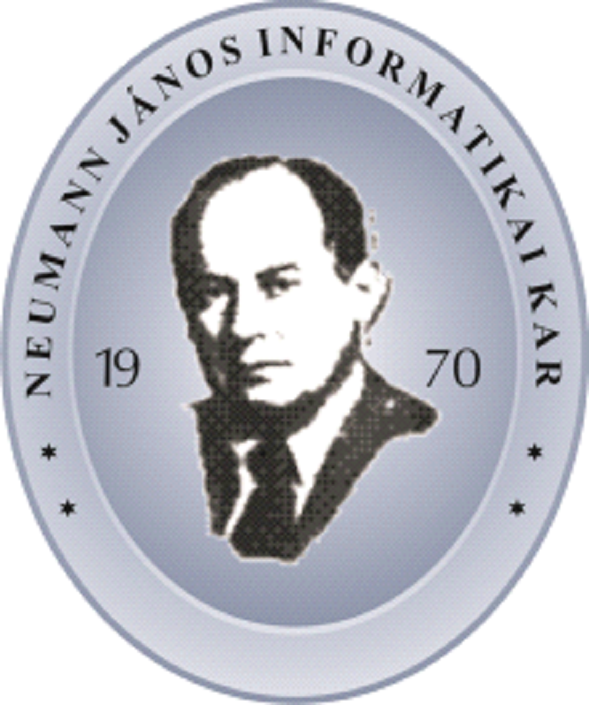
\includegraphics[width=.15\linewidth]{nik.png}
          \end{tabular}%
        }
		\vspace{0.5cm}			
		\begin{center}			
			
		      \topskip0pt
            \vspace*{\fill}
            \Huge
			     \textbf{SZAKDOLGOZAT}
            
            \vspace*{\fill}
            %
			
			
		
				
		\end{center}

    \begin{table}[htb]
    \centering
    \begin{tabular}{llr}
    \textbf{\begin{tabular}[c]{@{}l@{}}OE-NIK\\ 2023\end{tabular}} & \begin{tabular}[c]{@{}l@{}}Hallgatók neve:\\ Hallgatók törzskönyvi száma:\end{tabular} & \textbf{\begin{tabular}[c]{@{}r@{}}Hua Nam Anh\\ T/006785/FI12904/N\end{tabular}}       \\
                                                                   &                                                                                      & \textbf{\begin{tabular}[c]{@{}r@{}}Gaál Bernát Ruben\\ T/006756/FI12904/N\end{tabular}} \\
                                                                   &                                                                                      & \multicolumn{1}{l}{}                                                    
    \end{tabular}
    \end{table}
	\end{titlepage}
	\renewcommand*\contentsname{Tartalomjegyzék}
	\tableofcontents
	\newpage
	\par\noindent\rule{\textwidth}{0.4pt}
	\section*{Absztrakt}
     \emph{
		A közelmúltban a mélytanuláson alapuló 3D arcrekonstrukciós módszerek
		ígéretes eredményeket mutattak mind minőség, mind hatékonyság tekintetében. A neurális hálózatok tanítása azonban jellemzően nagy mennyiségű címkézett
		adatot igényel, ami magával vonzza a megfelelő erőforrásokat.
		A felsoroltak hiányában mi az alábbi megoldást javasoljuk. Egy gyengén
		felügyelt tanítású hálózatot, amit lehetséges kontrollálatlan környezetben készült képekkel betanítani.
		Ennek megvalósításához kettő már kész kutatás anyagát vettük igénybe. Az
		első, DECA \cite{deca} képes kezelni az arc kisebb részleteit, arckifejezéseit. A
		másik, a FOCUS \cite{focus} bemutatott egy korszerű megközelítést az arckép rekonstrukciójára kitakarások mellett. Ilyen kitakarások például a szemüveg és sapka. Ezek a kutatások nem csak korszerűek, de a NoW challenge teljesítményértekelései alapján bizonyítottan jól teljesítenek. Ezeket ötvözve egy robosztus, illetve realisztikus
		arcképek generálására alkalmas módszert mutatunk be ebben a tanulmányban.
		A rekonstrukció mellet implementáltunk egy arckép analízálására alkalmas módszert, amely képes eldönteni az arcképen lévő személy érzelmi
		állapotát és nemét. Ezek köré egy felhasználó barát mikroszerviz alapú web
		applikációt biztosítunk, melynek szolgáltatásai felhőn üzelmelnek.
		}
	\par\noindent\rule{\textwidth}{0.4pt}

    \section*{Abstract}
        \textit{Recently, 3D facial reconstruction methods based on deep learning have shown promising results in terms of both quality and efficiency. However, learning neural networks typically requires a large amount of labeled data, which entails corresponding resources.
        }
        \textit{In the absence of the above, we propose the following solution. A poorly supervised learning network that can be trained with images in an unsupervised environment.To implement this, we have drawn on the material of two existing research studies. From the first one, DECA \cite{deca}, is able to handle small details of the face and facial expressions. The other, FOCUS \cite{focus}, presented a state-of-the-art approach to facial reconstruction with occlusions. Examples of such masking are glasses and hats. These are not only state of the art, but have been shown to perform well in the NoW challenge performance tests. Combining them to create a robust and realistic generating realistic facial images is presented in this paper.}
        \textit{In addition to the reconstruction, we implemented a facial analysis method that can decide the emotional state and gender. These are built around a user friendly microservice based web application with services running on the cloud.}
     
	\par\noindent\rule{\textwidth}{0.4pt}

    \section{Bevezetés}
        Az elmúlt évek során egyre több figyelmet kaptak a digitális képfeldolgozáson alapuló technológiák az informatikában. 
        Mint ahogy Araceli Morales és tsai. \cite{survey} is megemlítették a munkájukban, az arcfelismerő technológiák széles körben elterjedtek napjainkban, beleértve a biztonságot, animációt és egészségügyet. 
        Illetve, ezen szakmai területen mostanság felkapott, hogy 3D-s adatok implementálásával megkerüljék a 2D arckép által megszabott határokat, mivel a 2D-s kép képtelen az emberi arc geometriájának eltárolására.
        A 3D arcfelismerés sokkal pontosabb adatokat ad vissza, például pózban és megvilágításban, amelyek hátulütői a 2D-nek. Azonban ennek is vannak hátrányai, hogy például sokkal nagyobb komplexitású képfeldolgozást igényel, ezáltal szűkítve a lehetőségeket.

        Az arcokat többféleképpen is lehet rögzíteni, például Stereo-vision rendszerekkel, amelyek két kamerát használnak. Ezek a kamerák ugyanarról az objektumról készítenek párhuzamosan képeket, majd ezeket összehasonlítva visszaadják a képen lévő egy pontnak a mélységét.

        Egy másik módszer a 3D lézerszkenner (pl. NextEngine, Cyberware), amelyet elsősorban ipari célokra fejlesztettek. Ipari termékek vizsgálatával szemben az emberi arc feltérképezéséhez több feltételt kell figyelembe venni. Mivel az emberi arc nem lehet teljesen mozdulatlan, fontos, hogy a szkenner által készített felvétel időintervalluma csekély legyen.

        Röviden: a lézerszkenner fényhullámokat szór az objektumra és ezek annak felszínéről visszaverődnek a szenzorra. A szenzor ezután kiszámítja az objektum felszínének távolságát az alapján, hogy mennyi idő alatt tette meg a teljes utat a hullám. Ezt a folyamatot $"Time\enspace of\enspace flight"$-nak szokás nevezni.

        A következő technológia a 3D-s adatok rögzítésére az RGB-D kamerák (pl. Kinect) használata. Ezek olyan RGB kamerák, amelyek rendelkeznek infravörös szenzorral, mely mélységi adatokat biztosít, ezáltal egy RGB képet ad vissza, amiben minden pixelhez tartozik egy mélységi érték.

        Ezek a módszerek mind megfelelnek 3D-s adatok gyűjtésére, azonban az első két megvalósítás hátránya, hogy előre megszabott feltételeknek megfelelő környezetet és drága felszereléseket igényelnek egy jó minőségű arc szkenneléshez. Ellenben, az RGB-D kamerák olcsóbbak és könnyebben használhatóak, de a minőség korlátozott.

        A fent említett megközelítések általában költséges optimalizálási folyamatot igényelnek a jó minőségű 3D-s arc visszanyerése érdekében. Két évtized telt el Blanz és Vetter \cite{blanzvetter} úttörő munkája óta, amely először mutatta be hogyan lehet egyetlen képből rekonstruálni az arc 3D-s geometriáját. Azóta a 3D arcrekonstrukciós módszerek rohamosan fejlődtek, de a korábbi modellek csak az arc durva alakját tudták rekonstruálni, és képtelenek voltak kinyerni az arckifejezéstől függő geometriai részleteket, mint például a ráncokat, amik fontosak a realisztikusság szempontjából.

        Később jöttek újabb modellek, melyek képesek voltak kiragadni a fent említett geometriai részleteket, azonban hátrányuk, hogy egy nagy volumenű, jó minőségű tanító adathalmazt követelnek. Illetve, egy másik hátrányuk, hogy inkonzisztens módon teljesítettek a kitakarásokkal szemben. A kitakarások mindenütt jelen vannak, és eleve nehezen kezelhetőek az alakjuk, megjelenésük és a pozíciójuk sokfélesége miatt. Ezáltal okozott probléma az, hogy az arcmodell alkalmazkodik az eltakart arcrégióhoz, és ennek eredményeként a rekonstruált arc torz lesz. Ezért nyitott kérdés marad annak eldöntése, hogy mely pixelek illeszkedjenek, és melyek ne illeszkedjenek az arcra egy 3D arc rekonstrukciója során kitakarások jelenlétében. A közelmúltban számos olyan módszert javasoltak, amelyek gyengén felügyelt tanítású konvolúciós neurális hálózatokat(CNN) használnak a hatékony, robosztus és a fent említett kihívásokat leküzdő arcrekonstrukció eléréséhez.

        Tehát, a jelenlegi monokuláris 3D arcrekonstrukciós módszerek képesek finom geometriai részleteket visszaadni, azonban számos megkötéssel küzdenek. Egyes módszerek olyan arcokat generálnak, amelyeket nem lehet valósághűen animálni, mivel nem modellezik, hogy hogyan változnak a ráncok az arckifejezésekkel. Más módszerek kiváló minőségű szkennelt arcokat használnak a tanításhoz és nem jól általánosíthatóak a természetes körülményekben készült képekre. A Yao Feng és tsai. \cite{deca} által bemutatott DECA modell a legelső olyan megközelítés, amely regresszálja a 3D arcformát és az animálható részleteket, amelyek egy személyre jellemzőek, de az arckifejezéssel változnak, ezáltal képesek az arc valósághű animálására.

        A kitakarásokkal szemben a legtöbb megközelítés a 3D arc illesztéséhez inverz renderelést alkalmaz egy adott eltakaró szegmentálásához. Ennek hátránya, hogy egy szegmentációs modellhez nagy mennyiségű címkézett adatra van szükség. Chunlu Li és tsai. \cite{focus} ezzel ellentétben egy olyan modellalapú megközelítést mutatnak be a 3D arc rekonstrukciójához, amely rendkívül robosztus az arcot kitakaró tényezőkkel szemben, de nem igényel semmilyen címkét a kitakarásokról a tanításhoz.

        Ebben a tanulmányban az a célunk, hogy egy olyan animálható 3D arcrekonstrukciós modellt készítsünk gyengén felügyelt tanulással, amely robosztus a kitakarások ellen a fent említett DECA és FOCUS modellek segítségével. Ezt kiegészítve bemutatunk egy arcképet elemző megoldást, mely visszaadja a célszemély érzelmi állapotát, illetve nemét. Észrevettük a munkánk elkészítése során, hogy a meglévő megoldásokat nehéz egy átlagos személynek kipróbálnia technikai tudás hiányában, így a fenti két szolgáltatás köré egy webapplikációt készítünk, amit felhőn üzelmeltetünk.\\

        Összefoglalva, ez a dokumentum az alábbi öt szempontot fogalmazza meg:
        \begin{itemize}
	       \item Bemutatunk egy CNN-alapú, egyetlen képen alapuló arcrekonstrukciós módszert, amely kihasználja a hibrid szintű képinformációt a gyengén felügyelt tanuláshoz.
	       \item Konzisztens műkődést biztosít különböző kitakarások mellet.
	       \item Egy természetes körülmények között készített 2D-s képből egy realisztikus 3D arcrekonstrukciót hozunk létre.
	       \item Egy arcelemzésre alkalmas megoldást, mely képes megállapítani a képen szereplő személy nemét, valamint érzelmi állapotát.
	       \item Webapplikáció elkészítése és a szolgáltatások megfelelő mükődése a felhőn.
        \end{itemize}

    \section{Előzetes kutatások}
	\subsection{Neurális hálózat}
    Ebben a fejezetben Abraham és tsai. \cite{ann} munkája alapján bemutatjuk a neurális hálózatok működését.
    
	\label{NN}
	Az emberi agy bizonyítja a hatalmas neurális hálózatok létezését, amelyek sikeresen végeznek el kognitív, észlelési és irányítási feladatokat. Ilyen számításigényes feladat például az arcfelismerés, a beszéd és a testmozgás. Az agy hatékonyan kihasználja a masszív párhuzamosságot, számítási struktúrája nagy mértékben párhuzamos, és jó információfeldolgozási képességgel rendelkezik.
	
    \begin{figure}[h]	
		\centering
		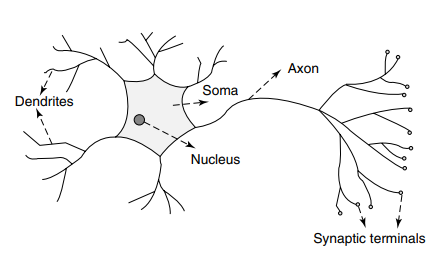
\includegraphics[width=0.8\linewidth]{neuron1}
		\caption{Neuron felépítése. 
			Forrás: \cite{ann}}
        \label{fig:neuron1}
	\end{figure}
 
	Az emberi agy több, mint 10 milliárd egymással összefüggő neuron gyűjteménye. Mindegyik neuron egy sejt (\ref{fig:neuron1}. ábra), amely biokémiai reakciókat használ az információ fogadáshoz, feldolgozáshoz és továbbításhoz.
	
	Az idegrostok faszerű hálózatai, az úgynevezett dendritek kapcsolódnak a sejttesthez, ahol a sejtmag található. A sejttestből egyetlen hosszú rost nyúlik, melyet \textit{axon}nak neveznek. Az \textit{axon} szálakra és alszálakra ágazik, majd szinapszisain keresztül kapcsolódik más neuronokhoz. Az itt létrejövő szinaptikus kapcsolat erőssége határozza meg az emberi agy tanulását .
	
	A jelek átvitele egyik neuronról a másikra a szinapszisoknál egy összetett kémiai folyamat, amelyben specifikus közvetítő anyagok szabadulnak fel a kapcsolódási pont küldői oldalán. A folyamat hatására a fogadó sejtben emelkedik vagy csökken az elektromos feszültség.
	
	\subsection{Mesterséges neurális hálózatok}
	A mesterséges neurális hálózatok (ANN-artificial neural networks) az előző fejezetben [\autoref{NN}] említett fejlettebb élő szervezetek agyát alkotó neuronokról kapták nevüket. 
	
	Mint azt Abraham és tsai. \cite{ann} is említik, a neurális hálózatok alapvető feldolgozási elemeit mesterséges neuronoknak nevezzük, vagy csak egyszerűen neuronoknak vagy csomópontoknak. A neuron leegyszerűsített matematikai modelljében a szinapszisok hatásai kapcsolati súlyokkal vannak reprezentálva, amelyek szabályozzák a bemeneti jelek hatását.
	
	A neuronok által mutatott nemlineáris karakterisztikát átviteli függvény segítségével ábrázoljuk. A neuron impulzusát ezután a bemeneti jelek súlyozott összegeként számíthatjuk ki az átviteli 
    függvénnyel transzformálva.
	 
	  Egy mesterséges neuron tanulási képessége a súlyok megfelelő beállításával érhető el egy választott tanító algoritmus felhasználásával.
	\newline
	
	Egy tipikus mesterséges neuron és egy többrétegű neurális hálózat modellezése a(z) \ref{fig:fig2}. ábrán látható. A(z) \ref{fig:fig2}. ábra szerint, ahogy a nyilak is mutatják, az $x_{1},...,x_{n}$ bemenetekről érkező jeláramlás egyirányúnak tekinthető csakúgy, mint a neuron kimeneti jelfolyama. A neuron kimeneti jelét \textit{O} a következő összefüggés adja:
	\begin{mdframed}
	\begin{align}
		&O = f(net) = f(\sum{j=1}^{n}w_{j}x_{j}) 
		\intertext{ahol $w_{j}$ a súly vektor és $f(net)$ az \textit{aktivációs} (átviteli) függvény. A \textit{net} változó a súly és a bementi vektorok skaláris szorzataként definiálható,}
		&net = w^{T}x = w_{1}x_{1} + ... + w_{n}x_{n}
		\intertext{ahol T egy mátrix transzponálását jelöli, és a legegyszerűbb esetben a kimeneti érték \textit{O} kiszámítható, mint}
		&O = f(net) = 
		\begin{cases}
			1,; ha ; w^{T}x ; \geq ; \theta \
			0, \text{különben} \
		\end{cases} \
	\end{align}
	ahol $\theta$-t \textit{küszöbszintnek} (threshold) nevezzük. Ezt a típusú aktivációs függvényt \textit{küszöb aktivációs függvénynek} nevezzük.
	
	\end{mdframed}
	
	
	\begin{figure}[h]%
		\centering
		\subfloat[\centering Mesterséges neuron]{{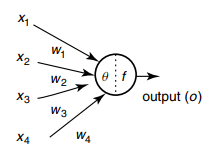
\includegraphics[width=5cm]{artificialNeuron} }}%
		\qquad
		\subfloat[\centering Többrétegű neurális háló]{{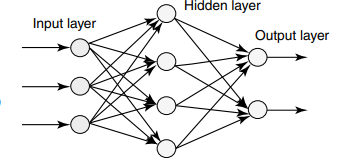
\includegraphics[width=5cm]{multilayered} }}%
		\caption{Mesterséges neuron felépítése és egy többrétegű neurális háló \newline\centering Forrás: \cite{ann}}%
		\label{fig:fig2}%
	\end{figure}
	\newpage
	A \textit{küszöbfüggvényhez} hasonlóan más aktivációs függvényekkel is előállítható az adott neuron bemenetre kapott válasz. Ilyen függvények a 
	\begin{itemize}
		\item lineáris,
		\item szigmoid,
		\item tangens hiperbolikusz.
	\end{itemize}

	\begin{figure}[h]	
		\centering
		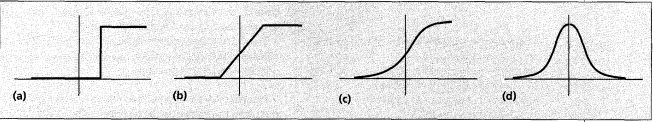
\includegraphics[width=1\linewidth]{fuggvenyek}
		\caption{(a) küszöbfüggvény, (b) lineáris, (c) szigmoid, (d) Gauss 
			\newline\centering Forrás: \cite{ann2}}
		\label{fuggvenyek}
	\end{figure}
    Az egyes aktivációs függvények a(z) \ref{fuggvenyek}. ábrán láthatóak.
 
	\clearpage
	\begin{mdframed}
	Ma az egyik leggyakrabban használt aktivációs függvény a szigmoid \cite{ann4}, melyet a következő képlettel határoznak meg:
	\begin{align}
		&y = \frac{1}{1 + e^{-(a - \theta)b}}
	\end{align}
	ahol \textit{a} az aktiválás, \textit{b} pedig a görbe alakját szabályozza.
	\end{mdframed}
	
	\subsection{Neurális hálózat architektúra}
	
	Bár a mesterséges neuron működési elvei és 
	egyszerű szabályrendszere elsőre talán nem tűnik érdekesnek, azonban e modellek teljes potenciálja és számítási teljesítménye akkor kel életre, 
	amikor mesterséges neurális hálózatokká
	kezdjük őket összekapcsolni (\ref{fig:fig2}. ábra). 
	Ezek a mesterséges neurális hálózatok 
	kihasználják az egyszerű tényt, 
	hogy a komplexitás néhány alapvető
	szabályból tud növekedni.
	
	A mesterséges neurális hálózatok 
	képesek komplex, valós problémák megoldására azáltal
	, hogy 
	alapvető építőelemeikben (\textit{mesterséges neuronok}) feldolgozzák az információt nemlineáris,
	elosztott, párhuzamos és lokális módon.
	
	Krenker és tsai. \cite{krenker} 
	   munkája alapján az egyes mesterséges 
	neuronok összekapcsolásának módját 
	\textit{topológiának}, \textit{architektúrának} 
	vagy \textit{gráfnak} nevezzük. A tény, 
	hogy az összekapcsolás
	számos lehetséges módon történhet több alkalmazható topológiát eredményez, amelyek két fő csoportra bonthatók. 

    \begin{figure}[h]	
		\centering
		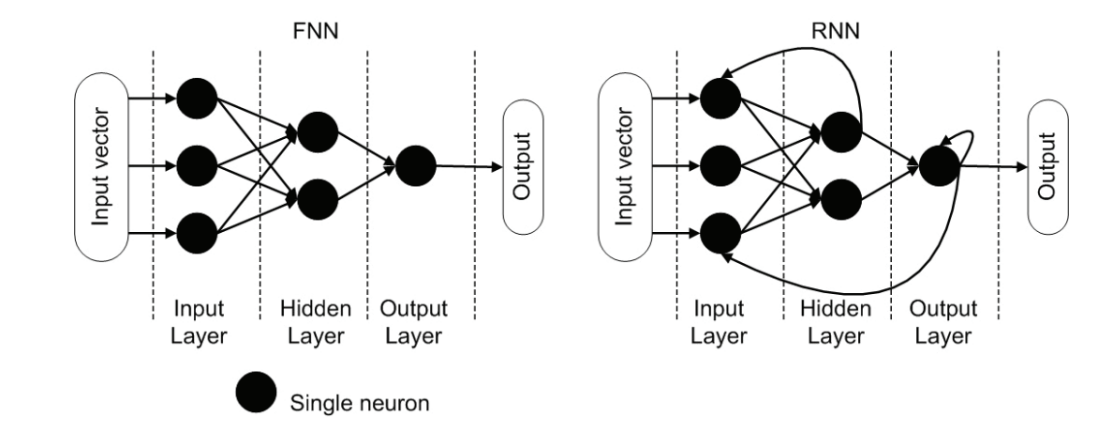
\includegraphics[width=1\linewidth]{topologies}
        
		\caption{Előrecsatolt (FNN) és rekurrens (RNN) \newline\centering  neurális hálózati topológiák. 
			Forrás: \cite{krenker}}
        \label{fig:topologies}
	\end{figure}
	
	A(z) \ref{fig:topologies}. ábra ezt a két topológiát mutatja. Az ábra bal oldala egy egyszerű előrecsatolt topológiát ábrázol, ahol az információ a bemenetekről kimenetekre áramlik egyirányúan. Az ábra jobb oldala pedig egy egyszerű rekurrens topológiát ábrázol, ahol az információ egy része nem csak egy irányban áramlik a bemenetről a kimenetre, hanem ellenkező irányban is.

	Fontos megemlíteni, hogy a mesterséges neurális hálózat könnyebb kezelése, és matematikai leírása érdekében az egyes neuronokat rétegekbe soroljuk. A(z) \ref{fig:topologies}. ábrán láthatjuk a bemeneti, a rejtett és a kimeneti réteget.
	
	A háló input rétegében minden neuron kapcsolatban áll a \textit{rejtett} (köztes) réteggel, így tovább adhatja a bemenetként kapott adatokat. A bemeneti réteg neuronjai súlyozott szinapszisokkal kapcsolódnak a belső rétegekhez.\\
	
	A mesterséges neurális hálózat 
	topológiájának kiválasztásával és 
	felépítésével még csak a feladataink 
	felét fejeztük be mielőtt a hálót az 
	adott probléma megoldására használhatnánk.
	Csakúgy, mint a biológiai neurális hálózatoknak
	is meg kell tanulniuk a megfelelő válaszokat különböző környezeti bemenetekre, a mesterséges neurális hálózatoknak is pontosan ezt kell tenniük.
	
	A következő lépés tehát, hogy \textit{betanítsuk} a mesterséges neurális hálózatot a helyes válaszokra.
	Erre négy lehetőségünk van:
	\begin{itemize}
		\item a felügyelt
		\item a felügyelet nélküli
		\item a megerősítéses
		\item és a hibrid
	\end{itemize}
	tanulás.
	
	 Függetlenül attól, hogy melyik módszert választjuk, a tanulás feladata, hogy a tanulási adatok alapján beállítsuk a súlyok és az előfeszítések értékeit, hogy minimalizáljuk a 
	költségfüggvényt.
	
	\subsection{Neurális hálók tanítása}
    Ebben a fejezetben Krenker és tsai. \cite{krenker} munkája alapján mutatjuk be a nerális hálózatok tanítási módszereit.
 
	A tanulási folyamat az ANN \cite{ann2} kontextusában a
	hálózat architektúrája és a kapcsolati súlyok frissítéseként értelmezhető annak érdekében, hogy a háló hatékonyan tudjon elvégezni egy adott feladatot.
	A hálózatnak a rendelkezésre álló tanító mintákból kell megtanulnia a kapcsolati súlyokat. A teljesítmény idővel javul a súlyok iteratív frissítésével.
	Az ANN-eket automatikus, példákból való tanulása teszi 
	vonzóvá és érdekessé. Szakértők által definiált szabályok helyett az ANN-ek a mögöttes szabályokat tanulják meg (pl. bemeneti-kimeneti kapcsolatokat) a megadott reprezentatív példák gyűjteményéből.
	
	\subsubsection{Felügyelt tanulás}
	
	A felügyelt tanulás egy olyan gépi tanulási technika, amely egy mesterséges neurális hálózat paramétereit tanítási
	adatokból állítja be. A tanuló ANN feladata, hogy beállítsa paramétereinek értékét bármely érvényes bemeneti értékre, miután látta a kimeneti értéket.
	A tanítási adatok a bementi és a kívánt kimeneti értékek párjaiból állnak, amelyeket adatvektorokban ábrázolnak.
	
	
	A felügyelt tanulást \textit{klasszifikációnak} is nevezhetjük, ahol \textit{osztályozók} széles skálája áll rendelkezésünkre, amelyek mindegyikének megvannak az erősségei és gyengeségei.
	A felügyelt tanulás egy
	adott problémájának megoldásához különböző lépéseket kell figyelembe venni.
	
	 Az első lépésben meg kell határoznunk a tanítási minták típusát. A második
	lépésben olyan tanítási adathalmazt kell gyűjtenünk, amely kielégítően leírja az adott problémát.
	A harmadik lépésben az összegyűjtött tanítási adathalmazt
	olyan formában kell leírnunk, amely érthető a kiválasztott ANN számára. A negyedik lépésben elvégezzük
	a tanítást. Ezután tesztelhetjük a tanult ANN teljesítményét a teszt (validációs) adathalmazzal.
	A validációs adathalmaz olyan adatokból áll, amelyeket a tanulás során nem vezettünk be a mesterséges neurális hálózatba.
	
	\subsubsection{Felügyelet nélküli tanulás}
	
	A felügyelet nélküli tanulás egy olyan gépi tanulási technika, amely egy ANN paramétereit megadott adatok és egy minimalizálandó 
	költségfüggvény alapján állítja be. A költségfüggvény bármilyen függvény lehet, amit a feladat határoz meg.
	
	
	Felügyelet nélküli tanulást leginkább olyan alkalmazásokban használnak, amelyek a becslési problémák körébe tartoznak, mint például a statisztikai modellezés, filterezés és a klaszterezés. A felügyelet 
	nélküli tanulás során arra törekszünk, hogy meghatározzuk, hogyan szerveződnek az adatok. Ez a felügyelt és a megerősítéses tanulástól abban különbözik, hogy az ANN csak \textit{címkézetlen} mintákat kap. A felügyelet nélküli tanulás egyik gyakori formája a klaszterezés, ahol az adatokat hasonlóságuk alapján próbáljuk különböző klaszterekbe sorolni.
	
	\subsubsection{Megerősítéses tanulás}
	
	A megerősítéses tanulás egy olyan gépi tanulási technika, amely egy olyan
	mesterséges neurális hálózat paramétereit állítja be, ahol általában az adatok nincsenek előre megadva, hanem a környezettel való kölcsönhatásokból generálódnak. A megerősítéses tanulás azzal foglalkozik, hogy egy mesterséges neurális hálózatnak hogyan kellene viselkednie egy adott környezetben annak érdekében, hogy maximalizálja a hosszú távú 
	eredményeket.
	
	Miután a maximalizálandó visszatérési függvényt meghatároztuk, a megerősítéses tanulás számos algoritmust használ a maximális visszatérést eredményező szabályok meghatározására. Az első lépésben egy naiv \textit{brute force} algoritmus kiszámítja a \textit{visszatérési függvény}t minden lehetséges szabályhoz, és kiválasztja azt, amelyik a legnagyobb visszatéréssel rendelkezik. Ennek az algoritmusnak nyilvánvaló gyengesége a rendkívül magas, vagy akár végtelen számú lehetséges szabály esetében rejlik. Ez a gyengeség kiküszöbölhető érték függvényes megközelítésekkel vagy közvetlen szabály becslésekkel. Az értékfüggvényes megközelítések megpróbálnak
	egy olyan szabályrendszert találni, amely maximalizálja a visszatérést.
	
	Ezek a módszerek konvergálnak a helyes becslésekhez egy rögzített szabály esetén és az optimális szabály megtalálására is használhatóak. Az értékfüggvényes megközelítéshez hasonlóan a közvetlen szabály becslés is képes megtalálni az optimális szabályt.

    \subsubsection{Átviteli tanítás}
    
     A hagyományos gépi tanulási módszerek \cite{tl} egyik feltételezése, hogy a tanítási és tesztelési adatok ugyanabból a tartományból származnak, így a bemeneti jellemzőtér és az adatok eloszlási jellemzői megegyeznek. Néhány valós gépi tanulási forgatókönyvben azonban ez a feltételezés nem áll fenn. Vannak olyan esetek, amikor a tanítási adatok gyűjtése drága vagy nehézkes. Ezért nagy teljesítményű tanulók létrehozására van szükség, amelyeket különböző tartományokból könnyebben beszerezhető adatokkal tanítanak. Ezt a módszert átviteli tanításnak nevezzük.

     Az átviteli tanítás alapvető célja a modell fejlesztésének felgyorsítása egy meglévő modellből kiindulva és annak tovább hangolása a specifikus problémára.
 
	\subsection{Konvolúciós neurális hálózatok}
	\begin{figure}[h]	
		\centering
		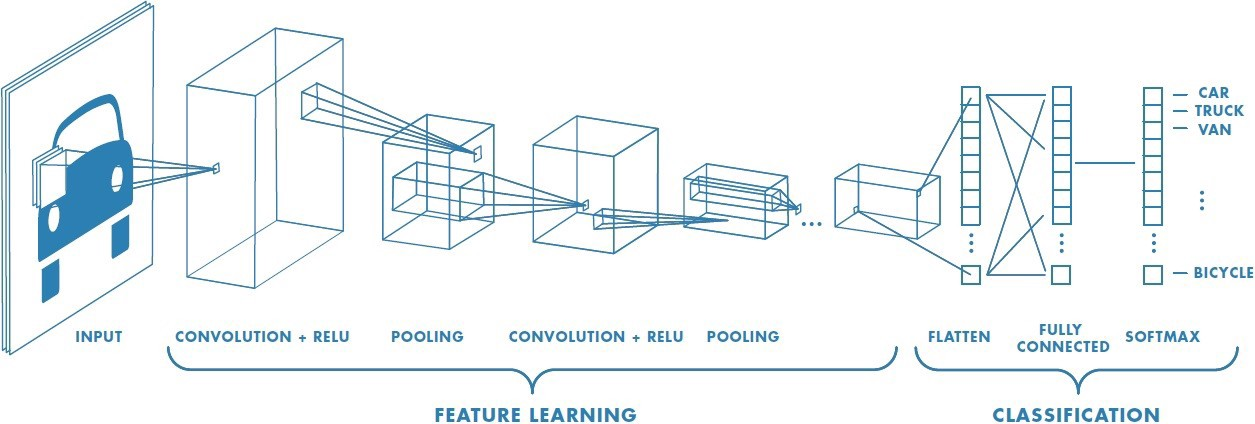
\includegraphics[width=1\linewidth]{CNN}
		\caption{CNN. Forrás: \cite{CNN}}
        \label{fig:cnn}
	\end{figure}
 
	Indolia és tsai. \cite{CNN} értelmezésében a konvolúciós neurális hálózat (CNN) (\ref{fig:cnn}. ábra) egy
	mélytanulási megközelítés, amelyet széles körben használnak komplex problémák megoldására és felülmúlja a hagyományos gépi tanulási megközelítéseket. A konvolúciós neurális hálózat mély előrecsatolt architektúrával rendelkezik és jobban képes általánosítani, mint a teljesen összekapcsolt rétegekkel rendelkező hálózatok.
	A CNN, mint a hierarchikus jellemző detektorok biológiailag inspirált koncepciója, képes nagymértékben megtanulni
	absztrakt jellemzőket és hatékonyan képes azonosítani az objektumokat.
	
	A CNN az alábbi előnyökkel rendelkezik más klasszikus modellekkel szemben:
	
	  A CNN-ek alkalmazásának legfőbb előnye a súlymegosztás koncepciójában rejlik, amelynek köszönhetően a 
    betanítandó paraméterek száma jelentősen csökken, ami jobb általánosításhoz vezet. 
	A kevesebb paraméter miatt a CNN egyszerűen betanítható és nem szenved túlillesztéstől. Az osztályozási szakasz beépül a jellemző kinyerési szakaszba. Mindkét szakasz használ tanulási folyamatot.A mesterséges neurális hálózat általános modelljeinek felhasználásával nagy hálózatokat sokkal nehezebb megvalósítani,
	mint CNN-ben.
	
	A CNN-eket széles körben használják különböző területeken figyelemreméltó
	teljesítményüknek köszönhetően, mint például a képosztályozás, a tárgyak felismerése, az arcfelismerés, a beszéd
	felismerés és a járműfelismerés.
	
	\subsubsection{A konvolúciós neurális hálózat általános modellje}
    Ebben a fejezetben Indolia és tsai. \cite{CNN} munkája alapján bemutatjuk a CNN-ek általános modelljét.
 
	\subsubsection{Általános modell}
	Az ANN általános modellje egyetlen bemeneti és kimeneti réteggel,
	valamint több rejtett réteggel rendelkezik.
	
	Egy bizonyos 
	neuron fogadja az X bemeneti vektort, és Y kimenetet állít elő azáltal,
	hogy valamilyen F függvényt hajt végre rajta az alábbi általános egyenlet [\ref{eq1}] alapján.
	\begin{mdframed}
	\begin{equation}
    \label{eq1}
			F(X, W) = Y
	\end{equation}
	,ahol W a súlyvektor, amely a két neuron közötti összeköttetés erősségét jelöli két szomszédos réteg között.
 	\end{mdframed}

	A kapott súlyvektor felhasználható a képosztályozáshoz.
	
	Jelentős mennyiségű irodalom létezik a képek pixelalapú osztályozásával
	kapcsolatban, azonban az olyan kontextuális információk, mint a kép alakja, vagy 
	a kép formája jobb eredményt adnak.
	
	A CNN a kontextuális információkon alapuló osztályozási képessége miatt kap egyre nagyobb figyelmet.\\
	
	
	A CNN általános modellje négy komponensből áll. Nevezetesen: 
	\begin{itemize}
		\item konvolúciós réteg
		\item összevonó réteg
		\item aktivációs függvény
		\item teljesen összekapcsolt réteg
	\end{itemize}

    \begin{figure}[h]	
		\centering
		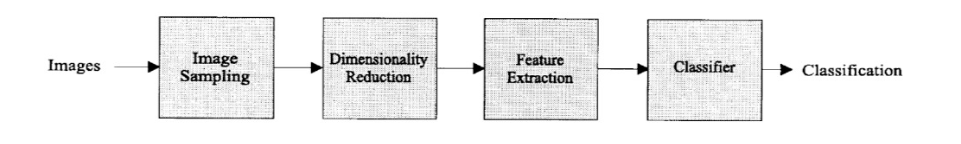
\includegraphics[width=1\linewidth]{element}
		\caption{A CNN elemi összetevői. Forrás: \cite{CNN}}
        \label{fig:cnnelem}
	\end{figure}
 
	Az egyes komponensek működését az alábbi \ref{fig:cnnelem}. ábra szemlélteti.

	
	\subsubsection{Konvolúciós réteg}
	
	Az osztályozandó képet a bemeneti rétegnek adjuk meg, a kimenet pedig az előre megjósolt osztálycímke, amelyet a képből kinyert jellemzők alapján számítunk ki.
	
	A következő rétegben lévő egyes neuronok az azt követő rétegben lévő neuronokhoz kapcsolódnak. Ezt a helyi korrelációt receptív mezőnek nevezzük.
	
    \begin{figure}[h]	
		\centering
		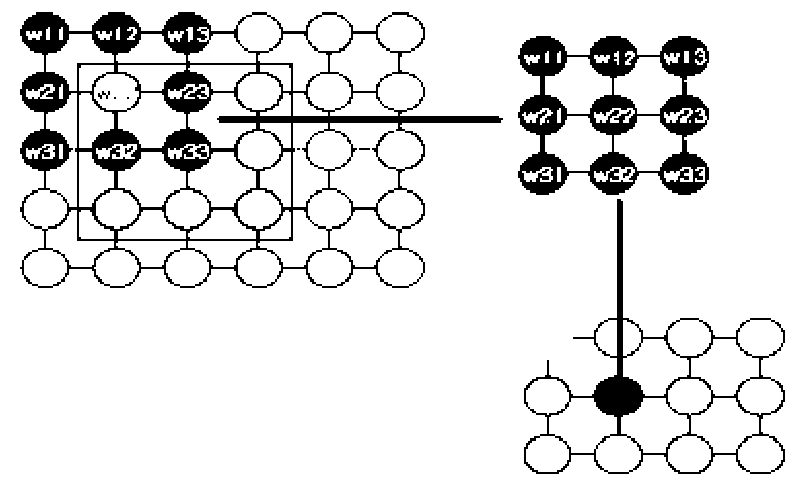
\includegraphics[width=0.7\linewidth]{receptiv}
		\caption{Az adott neuron receptív mezeje a következő rétegben. Forrás: \cite{CNN}}
        \label{fig:neuron-receptive}
	\end{figure}
 
	A bemeneti kép lokális jellemzőit a receptív mező (\ref{fig:neuron-receptive}. ábra) segítségével nyerjük ki. Az előző rétegben egy adott régióhoz tartozó neuron receptív mezeje egy súlyvektort alkot, amely a sík minden pontján egyenlő marad, ahol a sík a következő rétegben lévő neuronokra utal. Mivel a síkban lévő neuronok azonos súlyokkal rendelkeznek, így a különböző helyeken előforduló hasonló jellemzők a bemeneti adatokon belül felismerhetők.
	
		\newpage
	A súlyvektor, más néven szűrő vagy kernel a bemeneti vektoron csúszik át a jellemzőtérkép létrehozásához.
	A szűrő vízszintes és függőleges irányú csúsztatásának módszerét nevezzük konvolúciós műveletnek. A helyi receptív mező jelensége miatt a betanítható paraméterek száma jelentősen csökken.
	
	A következő rétegben az (i,j) helyhez tartozó $A_{ij}$ kimenet konvolúciós
	művelet alkalmazása után kerül kiszámításra az alábbi képlet segítségével:
	\begin{mdframed}
	\begin{align}
		a_{ij} = \sigma((W * X)_{ij} + b)
	\end{align}
	, ahol X a rétegnek adott bemenet, W a bemeneten áthaladó szűrő vagy kernel,
	b az eltolás, * a 
	a konvolúciós műveletet, és $\sigma$ a hálózatba bevezetett nemlinearitást jelöli.
	\end{mdframed}
	
	\subsubsection{Összevonó réteg}

	A konvolúciós réteget összevonó (pooling) vagy 
	almintavételező (sub-sampling) \cite{CNN} réteg követi.
	Az összevonó technika használatának fő előnye, hogy 
	jelentősen csökkenti a betanítható paraméterek számát,
	és bevezeti a fordítási invarianciát. 

    \begin{figure}[h]	
		\centering
		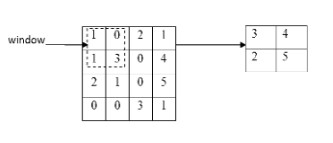
\includegraphics[width=0.5\linewidth]{pooling-op.jpg}
		\caption{2 x 2 ablak kiválasztásával végzett összevonási művelet. Forrás: \cite{CNN}}
        \label{fig:pooling}
	\end{figure}
 
	Az összevonás művelet elvégzéséhez kiválasztunk egy ablakot,
	és az abban az ablakban lévő bemeneti elemeket átadjuk
	egy összevonó függvénynek a(z) \ref{fig:pooling}. ábrán látható módon.
	
	\newpage
	
	A pooling függvény egy másik kimeneti vektort generál.
	
	Létezik néhány összevonási technika, mint például az átlagolt összevonás 
	és a \textit{max-pooling}, amelyek közül a \textit{max-pooling} a leggyakrabban használt módszer,
	mely jelentősen csökkenti a leképezés méretét.
	
	A hibák kiszámítása során a hiba nem terjed vissza a győztes egységre.
	
	\subsubsection{Teljesen összekapcsolt réteg}
	
	A teljesen összekapcsolt réteg \cite{CNN} hasonló a hagyományos modellek teljesen összekapcsolt hálózatához.
	
	Az első
	fázis kimenete (a konvolúciót és a összevonást ismétlődően tartalmazza) a teljesen összekapcsolt rétegbe kerül, és a súlyvektor és bemeneti vektor pontproduktumát számoljuk ki a végeredmény kiszámítása érdekében.
	
	A \textit{gradiens süllyedés}, más néven kötegelt módú tanulás vagy offline algoritmus, csökkenti a költségfüggvényt a költség becslésével egy teljes tanítási adathalmaz felett, és a paramétereket csak egy korszak után frissíti, ahol egy korszak a teljes adathalmaz átfutásának felel meg.
	Ez globális minimumokat eredményez, de ha a képzési adathalmaz mérete nagy, akkor a hálózat tanításához szükséges idő
	jelentősen megnő. A költségfüggvény csökkentésének ezt a megközelítését felváltotta a \textit{sztochasztikus gradiens süllyedés}.
 
	\subsubsection{Aktivációs függvény}
	
	Számos szakirodalom létezik, amely a hagyományos gépi tanulási algoritmusokban
	szigmoid aktivációs függvényt használ.
	A nemlinearitás bevezetése érdekében a Rectified Linear Unit (ReLU) használata jobbnak bizonyult az előbbinél
	két fő tényező miatt. 
	
	Először is, a ReLU parciális deriváltjának kiszámítása egyszerű. 
	Másodszor, miközben figyelembe vesszük
	a tanítási időt, mint az egyik tényezőt, a telítődő nemlinearitások, mint a szigmoid lassabbak, mint a nem telítődő nemlinearitások, mint a ReLU.
	 Harmadszor, ReLU nem engedi, hogy a gradiensek eltűnjenek, de a ReLU hatékonysága romlik, ha nagy gradiens áramlik át a hálózaton, és a súly frissítése miatt a neuron nem aktiválódik, ami a \textit{Dying ReLU} problémához vezet, amely egy jelentős probléma. 
	 
	 Ez a probléma megoldható a \textit{Leaky ReLU} segítségével, ha $x>0$, a függvény aktiválódik.
	mint $f(x)= x$, ha pedig $x<0$, akkor a függvény $\alpha x$-ként aktiválódik, ahol $\alpha$ egy kis konstans.

    \subsection{Reziduális Neurális Hálózatok}
    
    \begin{figure}[h]	
 		\centering
 		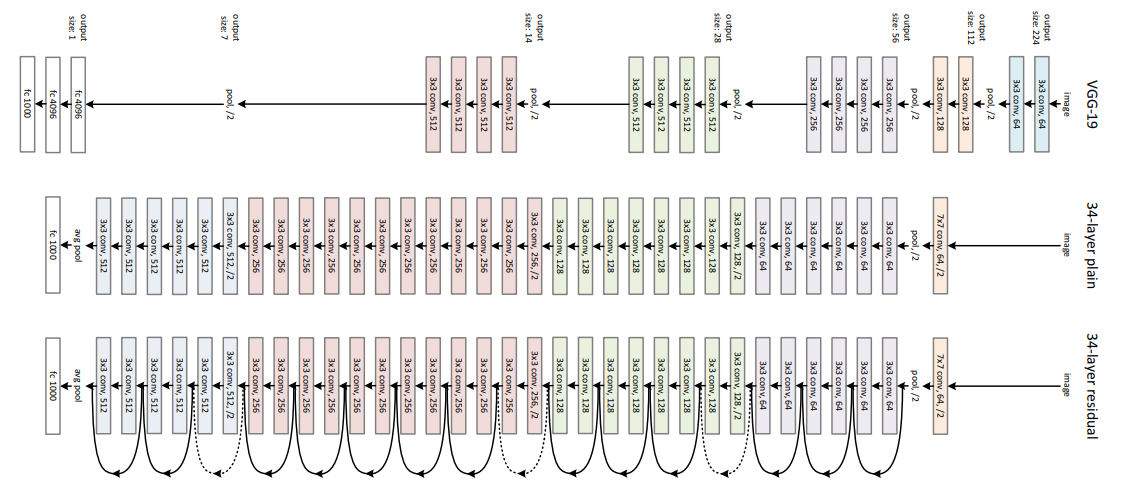
\includegraphics[width=1\linewidth]{ResNet}
 		\caption{ResNet architektúrák felépítése. (felülről a 3.)
 			Forrás: \cite{resnet}}
        \label{fig:resnet}
 	\end{figure}
    
    A mélyebb neurális hálózatok nehezebben taníthatóak. Amikor növeljük a rétegek számát, a mélytanulásban egy gyakori probléma merül fel, amit eltűnő/robbanó gradiensnek neveznek. Ennek hatására a gradiens 0 vagy túl nagy lesz. Így amikor növeljük a rétegek számát a hibaarány is nő. Ennek a problémának a megoldására He és tsai. \cite{resnet} bemutattak egy reziduális (maradékos) tanulási keretrendszert, amely megkönnyíti azon hálózatok tanítását, amelyek lényegesen mélyebbek a korábban használtakhoz képest. A rétegeket kifejezetten úgy alakították át, hogy a rétegek a réteg bemeneteire hivatkozva maradványfüggvényeket tanulnak a nem hivatkozott függvények helyett. Ezek a reziduális hálózatok könnyebben optimalizálhatók, és pontosságot nyerhetnek a jelentősen megnövelt mélységből fakadóan.
    A reziduális hálózatok általános felépítését a(z) \ref{fig:resnet}. ábra szemlélteti.

    \newpage
    \subsubsection{Reziduális blokkok}
    
    
    \begin{figure}[h]	
 		\centering
 		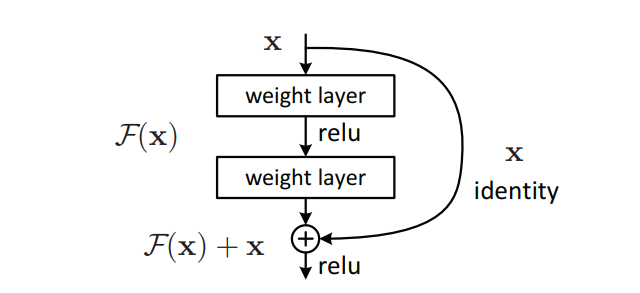
\includegraphics[width=1\linewidth]{Residual-Block}
 		\caption{He és tsai. által javasolt reziduális blokk felépítése.
 			Forrás: \cite{resnet}}
        \label{fig:resblock}
 	\end{figure}
  
    Az eltűnő gradiens problémájának megoldására bevezették a reziduális/maradék blokkokat (\ref{fig:resblock}. ábra). A hálózatban úgynevezett kihagyásos kapcsolatok jönnek létre. A kihagyásos kapcsolat egy réteg aktivációit úgy kapcsolja össze a további rétegekkel, hogy közben néhány réteget kihagy. Ez egy reziduális blokkot képez. A reziduális hálózatok ezen reziduális blokkok egymásra halmozásával jönnek létre. Az ilyen típusú kihagyásos kapcsolatok hozzáadásának előnye, hogy ha bármelyik réteg károsítja az architektúra teljesítményét, akkor azt a regularizáció kihagyja. Ez tehát egy nagyon mély neurális hálózat tanítását eredményezi az eltűnő gradiens okozta problémák nélkül. 


    A saját megvalósításunkban egy előtanított 50 rétegű reziduális hálózatot átviteli tanítással tanítottunk tovább, és finomhangoltuk azt a bemenetként átadott kép személyspecifikus jellemzőinek kinyerése érdekében.

    \subsection{3D arcmodell konstruálása}
        \label{3d}

        Ebben a fejezetben Morales és tsai. \cite{survey} munkája alapján bemutatásra kerülnek a 3D arcmodell konstruálására alkalmas modellek.
         A 3D-s arcok legelterjedtebb statisztikai modellje a 3D Morphable Models (3DMM), amelyet Blanz és Vetter \cite{blanzvetter} mutatott be a közösségnek. Bernhard és tsai. \cite{3dmm} munkája alapján a 3D Morphable Face Model egy generatív modell az arcformára
        és a megjelenés modellje, amely két kulcsfontosságú ötleten alapul:
    	 
    	  Először is, minden arc
    	sűrű pont-pont megfeleltetésben van, amelyet általában egy regisztrációs eljárás során egy sor példaarcon állítanak elő, majd
        a megfeleltetések a további feldolgozási lépések során is megmaradnak. Ennek a megfeleltetésnek köszönhetően az arcok lineáris kombinációi definiálhatók egy értelmes módon, morfológiailag valósághű arcokat (morfokat) létrehozva.
    	 
    	 
    	A második ötlet az arc alakjának és színének szétválasztása, és ezek függetlenítése a külső tényezőktől, például a megvilágítástól és a kamera paraméterektől.
    	 
    	  A \textit{morfológiai} modell magában foglalhat egy statisztikai modellt
    	  az arcok eloszlásáról, amely egy főkomponens elemzés az eredeti munkában.
       Egy lineáris
       alteret határoznak meg az alakzat és a textúra reprezentálására főkomponens elemzés \cite{PCA} segítségével, és bemutatják, hogyan lehet a modellt az adatokra illeszteni. 

	 \subsubsection{Arcképfelvétel}
        Minden 3D statisztikai arcmodell legfontosabb összetevője a 3D alakzatok reprezentatív készlete a megfelelő megjelenési adatokkal együtt. A mintakészlet létrehozásának tipikus módja, hogy az adatokat a valós világból kapjuk meg. Ebben a szakaszban rövid áttekintést adunk Egger és tsai. \cite{3dmm} munkája alapján a különböző megközelítésekről, amelyeket az arcadatok, valamint az arcképek adatainak megszerzésére használatosak.
	  
        A bemeneti adathalmazok létrehozása a 3DMM-ek számára kontrollált körülmények között történő felvételre korlátozódnak szemben a nagyobb kihívást jelentő kontrollálatlan felvételekkel.
	 
        Megjegyzendő, hogy a kontrollált 3D arcfelvétel nem mindig szükséges. Voltak kísérletek arra, hogy a 3DMM-eket közvetlenül képekből tanulják meg. Például Cashman és Fitzgibbon \cite{dolphins} munkája 2012-ben és a legmodernebb mélytanuláson alapuló módszerek egyszerre tanulnak 3DMM-et és regresszió-alapú illesztést 2D-s tanítási adatokból.
	 
	 \subsubsection{Alakfelvétel}
    	 Egger és tsai. \cite{3dmm} munkája alapján a háromdimenziós forma vitathatatlanul a 3DMM legfontosabb összetevője. Az alakzat ábrázolásának kérdése
    	 a 3DMM-ek összefüggésében nem került széles körben figyelembe vételre.
    	 
	   Messze a
	   leggyakrabban használt reprezentáció a háromszögháló. Vannak ritka kivételek, de ebben a munkában ezeket nem fogjuk megemlíteni.
	 
    A háromszöghálós reprezentáció sűrű megfeleltetéssel megköveteli, hogy minden minta azonos topológiát mutasson, és hogy a csúcsok minden mintán ugyanazt a szemantikai pontot kódolják. A minták közötti megfelelés megállapítása önmagában is kihívást jelentő téma. Ebben a szakaszban a nyers 3D adatokra összpontosítunk.
	
	
	\paragraph{Statisztika alapú modell illesztési módszerek}
    Ebben a szakaszban Morales és tsai. \cite{survey} munkája alapján bemutatásra kerülnek a statisztika alapú modell illesztési módszerek.
	
    A statisztikai 3D arcmodell a legnépszerűbb módszer az előzetes információ hozzáadására, mivel ezek kódolják az arc geometriai variációit, esetleg a megjelenéssel együtt.
	
	Az ilyen modellek tartalmaznak egy átlagos arcot, valamint annak geometriájának és az arcmintázatának a variációit és a megjelenését.
	 
	  3D arcmodell illesztése fényképre
	a modell paraméterein kívül,
	a 3D póz és a megvilágítás meghatározásával történik úgy, hogy
	az eredményül kapott 3D-s arc képsíkjába történő vetülete
	a lehető legjobban hasonlítson az adott képhez.
	
	\paragraph{Geometriai módszerekhez}
	A geometriai módszerek Egger és tsai. \cite{3dmm} megfogalmazásában közvetlenül becslik egy alakzat 3D-s koordinátáit, vagy ugyanazon felület megfigyelésével
	két vagy több nézőpontból (ebben az esetben a kihívás a megfelelő pontok azonosítása a képek között), vagy pedig egy vetített minta megfigyelésével (ebben az esetben a kihívás az ismert minta és a róla készült vetület kép közötti megfeleltetés azonosítása).
	
	A módszerek vagy aktívnak tekinthetők, azaz fényt
	vagy más jeleket sugároznak, vagy passzívak.
	
	
	A lézerszkennerek, a \textit{Time-of-Flight} érzékelők és a strukturált fényrendszerek \textit{aktív} rendszerek, míg a több nézetből álló fotogrammetria \textit{passzív} alternatíva.
	
	\paragraph{Fotometriai módszerek}
	A fotometriai módszerek \cite{3dmm} jellemzően a felület orientációját becslik, amelyből integrálással vissza lehet nyerni a 3D alakot.
	
    A kihívás itt az, hogy olyan modelleket válasszunk, amelyek pontosan megragadják a felszín reflexiós tulajdonságait, valamint elegendő mérési eredményt kapjunk ahhoz, hogy e modellek invertálása jól megoldható legyen. 
    
    A geometriai módszerekhez képest a fotometriai módszerek
    jellemzően nagyobb alaki részletességet kínálnak, és nem függnek az
    összeilleszthető jellemzők meglététől
    (tehát sima, jellegtelen felületek esetén is alkalmazhatóak), de gyakran szenvednek alacsony frekvenciájú torzításoktól a rekonstruált képekben
    a fényvisszaverő képesség és a megvilágítás modellezési hibái miatt.
    
    
    A fotometriai sztereót \cite{photometric} a felszín normálisa adja meg minden egyes képpontnál a jelenet rögzített pozícióból történő megfigyelésével, legalább három különböző megvilágítási körülmény között.
    
    A szükséges képkockák számát spektrális multiplexálással \cite{multiplex} lehet csökkenteni.
    	
	\paragraph{Hibrid módszerek}
	A hibrid módszerek \cite{3dmm} a
	geometriai és a fotometriai módszerek kombinációja. 
	
	Csökkentik a
	a fotometriai módszereknél jellemzően jelenlévő alacsony frekvenciájú torzítást, és
	növelik a nagyfrekvenciájú részleteket a geometriai módszerekhez képest. 
	
	Diego Nehab és tsai. \cite{hibrid} javaslata egy olyan módszer, amely helymeghatározó információk alacsony frekvenciáját egyesíti a felszíni normálisok magas frekvenciájával. 
	A módszer különösen hatékony, mivel csak egy lineáris egyenletrendszer megoldása szükséges.
    
    \subsection{Mélytanulási módszerek}
	
	Az előző szakasz [\nameref{3d}] 2D-ből 3D arc rekonstrukciós módszerei \textit{modelleket} használnak az előzetes tudás megtestesítésére \cite{survey}: a statisztikai modellillesztési módszerek tartalmaznak egy geometriai (és általában textúra) modellt, a fotometriai módszerek pedig a
	az arc fényvisszaverő képességét. 
	
	
	Ezzel szemben a mély tanulási módszerek
	közvetlenül tanulják meg a 2D kép és a 3D arc közötti leképezést, az előzetes ismeretek felhasználásával a betanított hálózatokban.
	
	
	Több indokból is előnyösebb mély tanulási módszerekkel dolgozni.\cite{3dmm}A modellezési oldalon a nemlineáris, mély reprezentációk használata lehetőséget nyújt arra, hogy felülmúljuk a klasszikus lineáris vagy multi-lineáris modelleket az általánosítás szempontjából, tömörség és specifikusság tekintetében \cite{styner}.
	
	
	A paraméter becslési oldalon ki tudjuk használni a mély hálózatok előnyeit, a gyorsaságot és a robusztusságot, hogy megbízható teljesítményt érjünk el a nem ellenőrzött képeken.
	
	\subsubsection{Mély arcrekonstrukciós modellek}
    Ebben az alfejezetben az mély arcmodellezési (deep face) módszereket mutatjuk be Egger és tsai. \cite{3dmm} munkája alapján. \\
 
	A hagyományos modellezési technikák célja, hogy
	az arc alakját, arckifejezését és megjelenését $w$ vektorként reprezentálják egy
	alacsony dimenziós látens térben $\mathbb{R}^d$ . A vetítés (illetve rekonstrukció) ebből a latens térből lineáris vagy multi lineáris műveletekkel definiálható, és úgy is felfogható, mint a nagy-dimenziós információ kódolása (ill.
	dekódolása) a $\mathbb{R}^d$ térben.
	
	
	A mélytanulás új eszközt nyújt a 3DMM-ek építéséhez, amely nemlinearitást használ mind a kódolóban és a dekódolóban. Az ilyen \textit{morphable} modellek létrehozása egy jelenleg nagyon aktív kutatási terület.
	Az alak és textúra modellezésre gyakran használt lineáris modellt felhasználva láthatjuk a mélytanulással és a hagyományos módszerekkel tanult kódoló és dekódoló közötti kapcsolatot.
	
	
	A mély tanulás kontextusában egy ilyen lineáris modell
	az alábbi egyenletben formalizálva pontosan megfelel egy teljesen összekapcsolt rétegnek egy
	neurális hálózatban.
	
	\begin{mdframed}
	\begin{equation}
		c(w) = \bar{c} + Ew 
	\end{equation}
		  ahol, $\bar{c}$ a tanítási adatokra számított átlag, $E \in \mathbb{R}^{3n*d}$ egy olyan mátrix, amely tartalmazza a $d$ legdominánsabb sajátvektorjait \\
		  a formakülönbségekre $c_i - \bar{c_i}$ számított kovarianciamátrixban és
		$w$ az alacsony dimenziós alakparaméter-vektor.
	\end{mdframed}
	
	Lényegében, a $w$ paramétervektora bemeneti jellemzők szerepét játssza, az $e_j$ főkomponensek pedig a súlyokét és az átlag $\bar{c}$ a torzítás.
	Ez úgy is felfogható, mint a dekódolás a latens paramétertérből a $c$ adattérbe. Vetítés a modellre
	hasonlóképpen tekinthető egy teljesen összekapcsolt réteggel történő kódolásnak,
	ahol a bemeneti jellemzők az adatok, a súlyok pedig a transzponált főkomponens mátrix sorai, az eltérések pedig adottak $-e^{T}_{j}\bar{c}$ által.
	
	
	 Az analógia lezárásaként a PCA (Principal Component Analysis) a kódoló és a dekódoló egyetlen rejtett réteggel rendelkező lineáris autokódolóvá történő kombinálásával végezhető el.
	Egy ilyen autokódoló $d$ neuronokkal a
	rejtett rétegben egy olyan látens teret fog megtanulni, amelynek kiterjedése megegyezik a $d$
	dimenziós PCA-val, bár az ortogonalitás garanciája nélkül.
	Ez megfelelő veszteségfüggvényekkel biztosítható.
	
	\subsubsection{Arcrekonstrukció mély neurális hálózatokkal}
	
	 A következőkben a mély neurális hálózatokon alapuló sűrű monokuláris arcrekonstrukció megközelítéseket tárgyaljuk. Megbeszéljük
	a felhasznált képzési adatokkal szemben támasztott követelményeket, valamint a különböző tanítási
	stratégiákat. 
	
	
	Nézzük meg először közelebbről a rekonstrukciós problémát. Blanz és Vetter \cite{blanzvetter} egy optimalizációs megközelítésen alapuló parametrikus modell illesztésével, azaz a gradiens süllyedéssel kezeli a monokuláris arc rekonstrukcióját. 
	
	 A mélytanulási megközelítések hasonló optimalizálási stratégiát követnek, de az optimalizálási probléma 
	tesztelés idején történő megoldása helyett például egy paraméterregresszort tanítanak be egy nagyméretű képadathalmaz alapján. A regresszor úgy értelmezhető, mint egy kódoló hálózat, amely egy 2D-s képet
	bemenetként fogad, és az alacsony dimenziós arcreprezentációt adja ki. 
	
	A
	kódolók kombinálhatók klasszikus arcmodelleken alapuló dekódolókkal,
	hogy végponttól-végpontig tartó kódoló-dekódoló architektúrákat hozzanak létre.
	Ez a módszertan széles körben elterjedt, és lehetővé teszi a klasszikus
	modellalapú és mélytanulási megközelítések ötvözését.
	
	\paragraph{Felügyelt rekonstrukció}
	Felügyelt regressziós megközelítések
	párosított tanítási adatok segítségével, azaz egy monokuláris  képgyűjtemény
	és a megfelelő 3DMM paraméterei segítségével tanulnak.
	
	Az egyik alapvető kérdés itt az, hogy hogyan lehet hatékonyan megszerezni az adatot egy ilyen felügyelt tanulási feladathoz. A következőkben
	kategorizáljuk a megközelítéseket a
	tanítási adatok alapján. \\
	
	Az egyik lehetőség az lenne, hogy a felhasználók határozzák meg az adatot. Míg ez egy népszerű stratégia, amelyet gyakran alkalmaznak rekonstrukciós problémáknál \cite{saragih}, 
	a sűrű geometria, a megjelenés és a helyszín megvilágítás pontos meghatározása szinte megoldhatatlan.
	
	Hasonló megközelítést alkalmaztak például Olszewski \cite{olszewski} munkájában,ahol három professzionális animátor kézzel készítette el a \textit{blendshape} animációt egy videokliphez illesztve. A sűrű rekonstrukciós feladatokhoz egyes megközelítéseket ellenőrzött, több nézetből készült felvételek alapján tanítanak be.
	
	Így megkapható az adat egy több nézetből történő rekonstrukciós megközelítéssel, amelyet egy 3DMM illesztése követ. Ezáltal megkapjuk a 3D adatot. Általában az alapadatok nagyon jó minőségűek,
	de a monokulárisan rögzített képek eloszlása nem
	egyezik meg a kontrollálatlan adatokkal, ami általánosítási problémákhoz vezethet
	a tesztelés idejében.\\
	
	Anh Tuan Tran \cite{tran} megközelítése monokuláris rekonstrukciót végez ugyanarról a személyről készült több képre, és kiszámít egy konszolidált arcazonosságot a 3DMM paraméterek egyszerű átlagolása alapján. \\
	
	Jelenleg a kutatóközösségben számos megközelítés szintetikus tanítási adatokat használ tanításhoz, mivel könnyen beszerezhető és tökéletes annotációkkal rendelkeznek. 
	
	Adott egy 3DMM arc, véletlenszerű identifikációk és kifejezések mintavételezhetők a paramétertérben. 
	Majd a modelleket véletlenszerű megvilágítási körülmények között, és különböző nézőpontokból lehet renderelni a monokuláris képek létrehozásához. 
	
	A háttértámogatást gyakran alkalmazzák úgy, hogy a generált arcokat a valós világ sokféle hátterére renderelik. Mivel az összes paramétert ellenőrzik, ezért azok kifejezetten ismertek és alapigazságként használhatók.
	
	Míg könnyen hozzájuthatunk a szintetikus tanítási adatokhoz, gyakran van egy nagy tartományi rés
	a szintetikus és a valós világ képei között, ami súlyosan befolyásolja
	a valós képekre való általánosítást. Például a hajat, az arcszőrzetet, a felsőtestet,
	vagy a száj belsejét gyakran egyáltalán nem modellezik. Az egyik lehetőség
	a jövőben olyan modelleket használni, amelyek tartalmazzák ezeket, hogy ellensúlyozzuk ezt a problémát. 
	
	A valós és a szintetikus tanítási adatok előnyeinek kihasználása érdekében számos jelenlegi megközelítést e két terület adatainak keverékével tanítanak. A cél itt az, hogy a megközelítés megtanulja kezelni a valós világi képeket, miközben a szintetikus tréning adatok tökéletes alapigazsága
	segítségével stabilizálható a tanulás.\\

	Ennek egy érdekes változata
	a tanítás önfelügyelt \textit{bootstrappelése}. A további megközelítéseket, amelyek tanítása nem igényel
	alapigazságadatokat a következő fejezetben vizsgáljuk meg.
	
	\paragraph{Önfelügyelt rekonstrukció}
	A konvolúciós neurális hálózatok felügyelt tanítása annotált adathalmazt igényel. A legtöbb
	eddig tárgyalt módszer ilyen - szintetikus vagy valós - adathalmazokat használ.
	
	A közelmúltban egyes megközelítések \cite{3dmm} önfelügyeletet alkalmazó
	tanulást használtak, azaz 3D címkék nélküli, valós képi adathalmazokon történő tanítást.
	Ezt az analízis-szintézis és a mélytanulási technikák kombinációja tette lehetővé.
	
	Tewari és tsai. \cite{tewari} egy modell-alapú kódoló-dekódoló architektúrát mutattak be, amely a
	a betanítható dekódolót egy fix dekódolóval helyettesíti. Ez a dekódoló a 3DMM paramétereket (látens kód)
	mint bemenet, amelyet a kódoló jelez a 3DMM segítségével 3D-rekonstrukcióvá alakítja.
	Továbbá szintetikus képet készít a rekonstrukcióról egy differenciálható renderelő segítségével.
	A rendereléshez szükséges külső paramétereket szintén a kódoló jelzi előre. 
	
	Az alkalmazott veszteségfüggvény nagyon hasonlít az analízis-szintézisben használthoz, ami fotometriai igazítást és statisztikai szabályozást foglal magába. Egy ilyen technikára úgy is gondolhatunk, mint egy közös analízis-szintézis optimalizálási probléma egy nagyméretű tanulási
	adathalmazon egyetlen kép helyett. Ez lehetővé teszi a paraméterregresszor tanítását 3D felügyelet nélkül.

    \subsection{Regularizáció}

        Ebben a fejezetben Tian és tsai. \cite{regularization-survey} munkája alapján bemutatjuk az általnunk használt fontosabb regularizációs módszereket.

        \begin{figure}[h]	
     		 \centering
     		 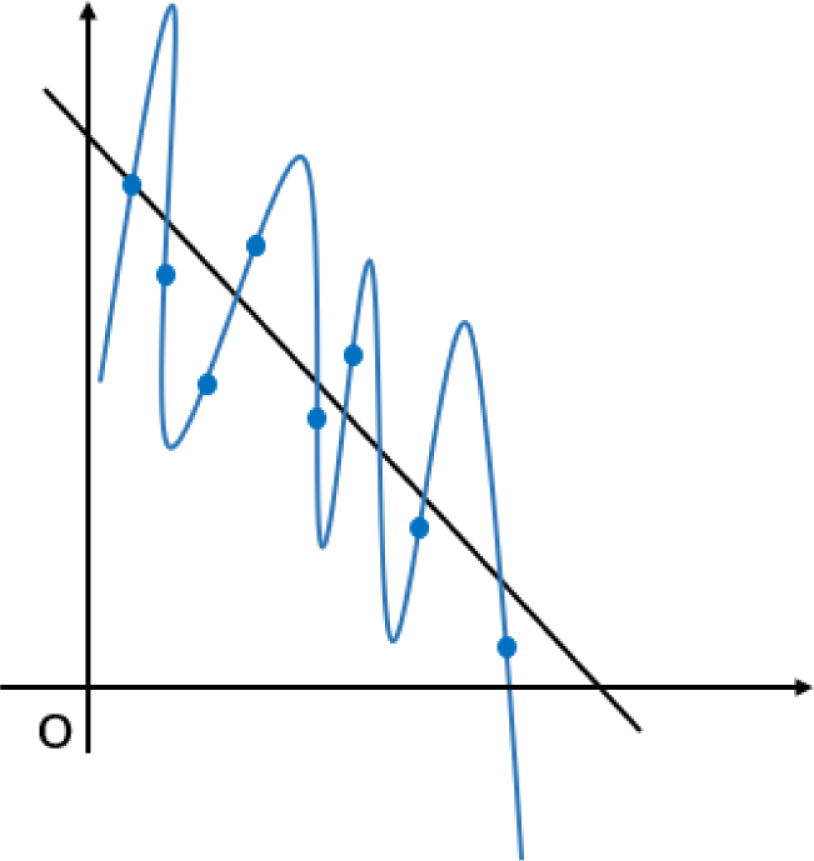
\includegraphics[width=0.5\linewidth]{overfitting.jpg}
     		 \caption{Példa túlillesztésre.
     			    Forrás: \cite{regularization-survey}}
                \label{fig:overfitting}
     	\end{figure}
        
        Egy nagyméretű modell betanítása kihívást jelentő probléma. Egy modell teljesítményét egy bizonyos tanítási adathalmazon maximalizáljuk. Az általánosíthatóságát az határozhatja meg, hogy képes-e jól teljesíteni a nem látott adatokon. A(z) \ref{fig:overfitting}. ábra példájaként az adatokra egy lineáris függvényt és egy polinomiális függvényt illesztünk. Bár a polinomiális függvény tökéletesebben illeszkedik az adatokhoz, míg a lineáris függvény jobb előrejelzéseket adhat a nem látott adatokra. A túlillesztés következtében a veszteség csökken a tanítási adatokon, ellenben nő a nem látott adatokon.

        A túlillesztés alapvető probléma a felügyelt gépi tanulásban az adatzaj jelenléte, a tanítási halmaz korlátozott mérete és az osztályozók összetettsége miatt. A regularizáció a gépi tanulás kulcsfontosságú eleme, amely lehetővé teszi a jó általánosítást a nem látott adatokra még akkor is, ha véges tanulóhalmazon vagy nem megfelelő iterációval történik a tanítás.

        A regularizálás a minimalizálandó célfüggvényhez néhány olyan megkötést ad, ami nem nyerhető ki az adatokból, és az előzetes preferenciát képviseli.

        A regularizáció minden olyan kiegészítő technika, amelynek célja a modell általánosításának javítása, azaz jobb eredmények elérése a tesztkészleten.

        A kötegelt normalizálás egy olyan operátor, amely normalizálja a rétegválaszokat az egyes mini kötegeken belül. Széles körben használják számos modern neurális hálózatban. Általában azt találják, hogy a kötegelt normalizálás javíthatja az általánosítási teljesítményt. Kötegelt normalizálást használunk például a dekódoló hálózatunkban is.

        A munkánk során alapvetően két fajta regularizációs módszert alkalmaztunk. Ezek a regularizációs  módszerek a \textit{ritkavektor-alapú regularizáció} és a \textit{ritkamátrix-alapú regularizáció}.

        Számos gyakorlati probléma, például a jellemzőválasztás, a ritka jelek szétválasztása és a ritka PCA során bizonyos változóknak ritkának kell lenniük. A ritka változó olyan változó, amelynek értékei többnyire nullát vesznek fel. A ritkított regularizáció általában büntetést érvényesít a változókra.
        
        \subsubsection{Ritkavektor-alapú regularizáció}
        Az $l_{0}$ norma ($|| x ||_{0}$) az $x$ vektor nem nulla összetevőinek számát határozza meg.
        
        Az $l_{1}$ norma a következőképpen definiálható:
        \begin{equation}
            ||x||_{1} = \sum_{j=1}^{N}|x_{j}|
        \end{equation}
        , ahol $x_{j} \in x$. Az $l_{1}$ norma regularizációval könnyen megoldhatóak konvex optimalizálási problémák, azonban torzítást eredményez a nagy együtthatók esetében.

        Az $l_{0}$ norma és az $l_{1}$ norma közötti szakadék áthidalása érdekében jelentős érdeklődés mutatkozik a nemkonvex $l_{p}$ norma használata iránt. Az $l_{p}$ norma kiszámítható, mint:
        \begin{equation}
            || x ||_{p} = (\sum_{j = 1}^{N}|x_{j}|^{p})^{\frac{1}{p}}
        \end{equation}
        , ahol $x_{j} \in x$ és $0 < p < 1$. 

        
        \subsubsection{Ritkamátrix-alapú regularizáció}
        A nagy kovariancia- vagy inverz kovariancia-mátrixok becslése a közelmúltban egyre nagyobb hangsúlyt kapott a nagydimenziós adatok elterjedtsége miatt.

        Egy mátrix $l_{2,1}$ normáját először az $l_{1}$ norma forgatási invariánsaként vezették be, amelyet a kiugró értékekkel szembeni robusztusság nehézségeinek leküzdésére javasolnak.

        Egy mátrix $l_{2,1}$ normája meghatározható, mint:
        \begin{equation}
            M(X) = ||X||_{2,1} = \sum_{j=1}^{n}(\sum_{i=1}^{m}X_{ij}^{2})^{\frac{1}{2}}
        \end{equation}
        , ahol $X_{ij} \in X$. A $p,q>=1$ értékekre az $l_{2,1}$ általánosított formája megadható, mint
        \begin{equation}
            M(X) = ||X||_{p,q} = (\sum_{j=1}^{n}(\sum_{i=1}^{m}X_{ij}^{p})^{\frac{q}{p}})^{\frac{1}{q}}
        \end{equation}
    
    
    \section{Kapcsolódó kutatások}

        Ahogy láthatjuk, a fellépő komplex kihívásokat különböző munkák minél kreatívabb megközelítéssekkel kísérelték meg legyőzni. Ezekről tovább Vetter és Blanz \cite{blanzvetter} munkájában és további dokumentumokban lehet olvasni. Ebben a fejezetben megvizsgáljuk a Yao Feng és tsai. \cite{deca} valamint Chunlu Li és tsai. \cite{focus} által bemutatott megközelítéseket, és megnézzük, hogy miért is fontosak a mi munkánk szempontjából.

        \subsection{DECA} \label{DECA}
 	
            Yao Feng és tsai. \cite{deca} az egyetlen kontrollálatlan környezetben készült 2D-s képből rekonstruált, animálható 3D fejmodell készítése érdekében fejlesztették ki a DECA (Detailed Expression Capture And Animation) modelljét. Egy kontrollálatlan környezetben készült képekkel tanított animálható elmozdulási modellt javasolnak, amely az arckifejezési paraméterek változtatásával képes hiteles geometriai részletek előállítására. Az előbbi cél elérése érdekében egy újszerű részletkonzisztencia költségfüggvényt mutatnak be a statikus és az arckifejezésekre dinamikusan változó geometriai adatok szétválasztására. Ammennyiben a tanítás során két kép érkezik különböző arckifejezésekkel, megfigyelhető, hogy a 3D arcformájuk és a személyspecifikus részleteik megegyeznek. Ezt a megfigyelést használják ki a részletkódok felcserélésével az azonos személyről készült különböző képek között és kikényszerítik, hogy az újonnan renderelt eredmények úgy nézzenek ki, mint az eredeti, bemenetként átadott képek. A geometriai részletek rekonstrukciója robosztus a jellemző kitakarásokra, a pózok nagyfokú változására és a megvilágítási variációkra.
    
            Egy olyan módszert mutatnak be, amellyel egyetlen természetes körülmények között rögzített 2D-s képből részletes és animálható 3D-s arcmodell hozható létre. A szerzők kétlépcsős megközelítést javasolnak: először egy 2D-s arcmezőkön betanított neurális hálózat segítségével megbecslik az arc 3D-s geometriáját, majd egy másik, már betanított deformációs modellen alapuló neurális hálózat segítségével részletekkel egészítik ki a 3D-s modellt.
    
            A szerzők megközelítése a FLAME modellen alapul. Ez egy parametrikus modell, amely az arc alakját és textúráját reprezentálja. A FLAME modellt a 3D-modell sablonjaként használják, és a becsült 3D-geometriát úgy deformálják, hogy az megfeleljen a bemeneti képen szereplő konkrét arcnak. Egy olyan módszert is javasolnak az arc tájékozódási pontjainak előrejelzésére a bemeneti képből, amely lehetővé teszi az arcmodell természetesnek tűnő arckifejezésekkel történő animálását.
    
        
     	      A továbbiakban megvizsgáljuk a DECA modell működési elvét és architektúráját.

            \begin{figure}[h]	
     		 \centering
     		 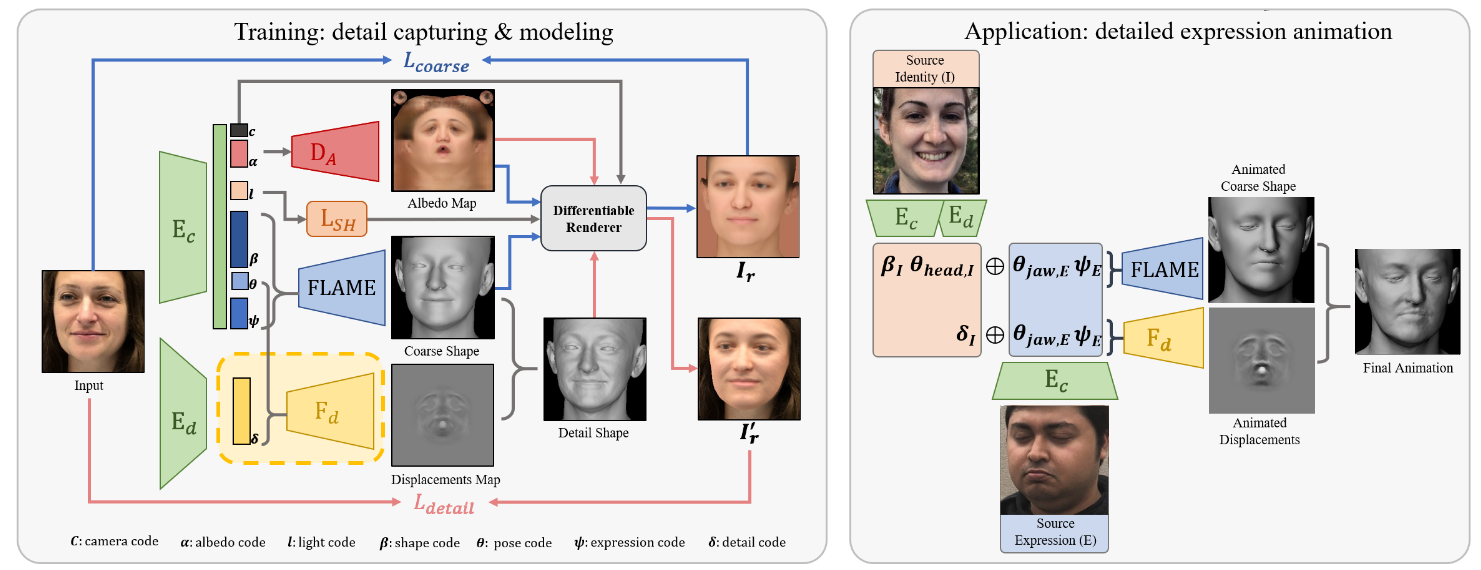
\includegraphics[width=1\linewidth]{deca}
     		 \caption{ DECA tanítás és animáció.
     			    Forrás: \cite{deca}}
                \label{fig:deca}
     	      \end{figure}

            \subsubsection{Kódoló} \label{Kódoló}
    	        Első lépésként egy durva rekonstrukciót a FLAME modelltérben \cite{flame}
                tanítanak be analízis-szintézis módon: egy bemenetként átadott \textit{I} 2D-s képből látens kódot készítenek, ezt dekódolják annak érdekében, hogy egy $I_{r}$ 2D-s képet hozzanak létre, valamint minimalizálják a szintetizált és a bemeneti kép közötti különbséget.
            
    	        A(z) \ref{fig:deca}. ábrán látható módon, egy $E_{c}$ kódolót tanítanak be, amely egy ResNet50 \cite{liwen} hálózatból, és egy azt követő teljesen összekapcsolt rétegből áll egy alacsony dimenziós látens kód regressziója céljából. Ez a látens kód tartalmazza a $\omega$ (identitás), $\psi$ (arckifejezés), $\theta$ (póz) FLAME \cite{flame} paramétereket (azaz reprezentálja a durva geometriát), az albedó együtthatókat $\alpha$, a kamera $c$ és a megvilágítási $l$ paramétereket.
    
                A durva rekonstrukcióhoz hasonlóan egy $E_{d}$ kódolót is betanítanak (amelynek architektúrája megegyezik a $E_{c}$-vel), hogy a bemeneti képet egy 128 dimenziós látens kódba kódolja, amely a személyre jellemző részleteket reprezentálja. 
    
    
                A kódolás folyamata a következőképpen mükődik:
                \begin{itemize}
    	           \item A bemeneti kép először egy sor konvolúciós rétegen halad át, amelyek magas szintű jellemzőket vonnak ki a képből. Minden egyes konvolúciós réteget egy csoportos normalizáló réteg és egy aktivációs függvény követ a normalizáláshoz és a nemlinearitás bevezetéséhez a konvolúciós réteg kimenetén.
                
    	           \item A konvolúciós rétegek kimenetét ezután kilapítják és egy teljesen összekapcsolt rétegen vezetik át, ami csökkenti a jellemzővektor dimenzióját.
                
    	           \item A teljesen összekapcsolt réteg kimenete ezután több további teljesen összekapcsolt rétegen halad át, amelyek mindegyikét egy tételes normalizáló réteg és egy aktivációs függvény követi. Ezek a rétegek a jellemzővektort egy alacsonyabb dimenziós látens kódra képezik le a látens térben.
                
    	           \item Az utolsó, teljesen összekapcsolt réteg kimenete a látens kód.
    	           
                \end{itemize}
    
            \subsubsection{Dekódoló} \label{Dekódoló}
    
                A dekódolási folyamat során a bemeneti látens kód először egy sor teljesen összekapcsolt rétegen halad át, hogy egy nagydimenziós jellemzővektort hozzon létre. Ezt a jellemzővektort ezután egy 3D-s tenzor alakjára alakítják át, majd egy sor dekonvolúciós rétegen vezetik át a tenzor felskálázásához és a kimeneti kép előállítása érdekében.
    
                A dekódoló dekonvolúciós rétegei lényegében a kódoló konvolúciós rétegeinek ellentétes műveletét végzik, azaz a bemeneti tenzort nagyobb felbontásra mintavételezik. Az egyes dekonvolúciós rétegek kimenete egy csoportos normalizáló rétegen és egy aktivációs függvényen halad át a nemlinearitás bevezetése és a kimenet normalizálása érdekében.
    
                A dekódoló végső kimenete a kívánt pózt tartalmazó rekonstruált kép. A dekódoló hálózat egy részletes $UV$ elmozdulási térképpel $D$ egészíti ki a durva $FLAME$ geometriát. A látens kódot $\delta$
     	        a $FLAME$ $\psi$ arckifejezés és állkapocs póz $\theta_{jaw}$ paramétereivel kapcsolják
     	          össze, majd $F_{d}$ az imént említett paraméterekből előállítja $D$-t. 
                $F_{d}$ a látens kódot $\delta$ felhasználva szabályozza a statikus személyspecifikus részleteket. Kihasználja a durva rekonstrukcióból kapott arckifejezés $\psi$ és az állkapocs $\theta_{jaw}$ paramétereket a dinamikus, kifejezésektől függő ráncok részleteinek rögzítése érdekében. A rendereléshez $D$-t normáltérképpé alakítják.

            \subsubsection{Részletkonzisztencia veszteség}
    	 
        	    \begin{figure}[h]	
        	 	     \centering
        	 	     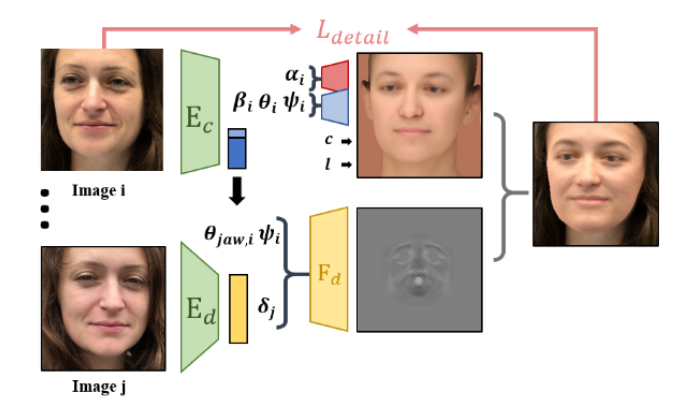
\includegraphics[width=1\linewidth]{ldetail}
        	 	     \caption{Részletkonzisztencia veszteség \\
        	 		    Forrás: \cite{deca}}
                  \label{fig:ldetail}
    	        \end{figure}
    
                Yao Feng és tsai. az identitás-függő és a kifejezésektől függő részletek
     	        szétválasztása érdekében egy új részletkonzisztencia veszteség függvényt (\ref{fig:ldetail}. ábra)
     	        javasolnak. A metódus nélkül a személyspecifikus látens kód $\delta$ rögzíti az
                identitástól és a kifejezésektől függő részleteket. 
                Ebből kifolyólag a rekonstruált részletek nem repozicionálhatóak a FLAME állkapocs póz $\theta_{jaw}$ és arckifejezés $\psi$ paramétereinek megváltoztatásával. Amennyiben adott két kép $I_{i}$ és $I_{j}$ ugyanarról az alanyról ($c_{i} = c_{j}$), a veszteséget a következőképpen határozzuk meg:
        
                \begin{equation*}
                L_{dc} = L_{detail}(I_{i}, R(M (\beta_{i}, \theta_{i}, \psi_{i}), A(\alpha_{i}), F_{d}(\delta_{j} , \psi_{i}, \theta_{jaw,i}), l_{i}, c_{i}))
                \end{equation*}
            
         	      , ahol $\beta_{i},$ $\theta_{i},$ $\theta_{jaw,i},$ $\alpha_{i},$ és 
                $c_{i}$ $I_{i}$ paraméterei, valamint $\delta_{j}$ $I_{j}$ részletkódja.

            \subsubsection{Tanítás}
                Ebben az alfejezetben a(z) \ref{fig:deca}. ábrán szemléltetett $DECA$ modellt vizsgáljuk meg.
     	          A tanítás során (bal oldali doboz) a $DECA$ minden egyes képhez
     	          az arc alakjának rekonstruálásához szükséges paramétereket becsli meg az
     	          alakkonzisztencia információ segítségével (a kék nyilakat követve), majd
     	          a részletkonzisztenica információ (a piros nyilakat követve) kihasználásával
     	          megtanul egy kifejezésfüggő elmozdulási modellt. A sárga doboz tartalmazza
     	          az elmozdulási konzisztencia-veszteséget, amelyet részletesebben
                a(z) \ref{fig:ldetail}. ábra szemléltet.
     	          A tanítás után a $DECA$ animál egy arcot [\ref{fig:deca}. ábra, 
                jobb oldali doboz] a rekonstruált forrásidentitás alakjának, fejpózának, részletkódjának, valamint a forráskifejezés állkapocs pózának és arckifejezési paramétereinek kombinálásával annak érdekében, hogy egy animált durva alakot és elmozdulási térképet kapjon. A modell kimenete egy animált
     	          részletes alakzat.

                A betanítási folyamat a következő lépésekből áll:
                    \begin{itemize}
                        \item \textbf{Az adatok előfeldolgozása}: Az adatok előfeldolgozása annak biztosítása érdekében, hogy azok megfelelően igazodjanak és normalizálódjanak, valamint átméretezzék és körülvágják az arcot.
    
                        \item \textbf{Kódolás} Ahogy a fentiekben említettük [\ref{Kódoló}], a DECA modell egy kódolót használ a bemeneti arc alacsony dimenziós reprezentációjává alakításához. 
    
                        \item \textbf{Dekódolás} Ahogy a fentiekben említettük [\ref{Dekódoló}], az alacsony dimenziós reprezentációt ezután egy dekódolóba táplálják, amely rekonstruálja az eredeti arcot egy adott arckifejezéssel
    
                        \item \textbf{Veszteségfüggvény}: A rekonstruált arc és a bemeneti arc közötti különbséget több veszteségfüggvény segítségével számszerűsítik. Ezek a veszteségfüggvények a neurális hálózat súlyainak beállítására szolgálnak, hogy minimalizálják a rekonstruált arc és a bemeneti arc közötti különbséget.
    
                        \item \textbf{hiba-visszaterjesztés}: A neurális hálózat súlyainak frissítése hiba-visszaterjesztéssel történik, amely a veszteségfüggvény gradiensének kiszámítását jelenti a súlyok tekintetében, valamint a súlyok ennek megfelelő beállítását.
    
                        \item \textbf{Iteratív tanítás}: A tanítási folyamatot több cikluson keresztül addig ismétlik, amíg a modell nem konvergál egy megfelelő teljesítményszintre.
                    \end{itemize}
                
            \subsubsection{Adathalmazok}
                A $DECA$-t három nyilvánosan elérhető adathalmazon tanítják:
     	              \begin{itemize}
     	            	\item VGGFACE2
     	            	\item BUPT-Balancedface
     	            	\item VoxCeleb2
     	              \end{itemize}
    
                A VGGFace2 több, mint 8 ezer alany képeit tartalmazza átlagosan több,
     	          mint 350 képpel alanyonként. A BUPT-Balancedface 7 ezer képet kínál
     	          etnikumonként, a VoxCeleb2 pedig 145 ezer videót tartalmaz 6 ezer
     	          különböző alanyról. Összességében a DECA-t több, mint 2 millió képpel tanították
     	          be.

            \subsubsection{FLAME modell}

                Mint ahogy korábbiakban említettük a \ref{DECA} fejezetben, a javasolt módszerben a FLAME modellt szintetikus 3D-s arcok generálására használják az arckifejezések, a póz és a fényviszonyok variációival. Ezeket a szintetikus arcokat ezután a valós világbeli képekkel együtt egy mély neurális hálózat betanítására használják, amely képes megjósolni a FLAME modell paramétereit egy bemeneti kép alapján.

                A FLAME modell Tianye és tsai. \cite{flame} munkája alapján egy statisztikai fejmodell, ami pontosabb és kifejezőbb mint a korábbi fej- és arcmodellek, miközben kompatibilis marad a szabványos grafikus szoftverekkel. A már meglévő modellekkel ellentétben a FLAME explicit módon modellezi a fej tartását és a szemgolyó forgását.

                A FLAME egyesíti a különálló lináris identitásalak és kifejezés tereket $linear$ $blend$ $skinning$-gel (LBS) és a pózfüggő korrektív $blendshape$ alakzatokat annak érdekében, hogy a nyak, az állkapocs és a szemgolyók mozgathatóak legyenek. Adott arc identitás $\beta \in R^{|\beta|}$, póz $\theta \in R^{3k+3}$ (ahol $k = 4$ a nyak, állkapocs, és szemgolyók ízületeinek száma), és arckifejezés $\psi \in R^{|\psi|}$ paraméterek mellett, a FLAME egy $n = 5023 $ csúcspontot tartalmazó archálót ad kimenetül.

                A modell a következőképpen van definiálva: 

                \begin{equation*}
                    M (\beta, \theta, \psi) = W (T_{p}(\beta, \theta, \psi), J(\beta), \theta, W)
                \end{equation*}

                ahol, a $blendskinning$ függvény $W (T, J, θ, W)$ elforgatja a  $T \in R^{3n}$ csúcsait a $J \in R^{3k}$ ízületek körül, lineárisan finomítva a $W \in R^{k\times n}$ keverési súlyokkal. A $J$ ízületi helyek a $\beta$ identitás függvényeként definiálhatók.

                Továbbá, 
                \begin{equation*}
                    T_{p}(\beta, \theta, \psi) = T + B_{S}(\beta, S) + B_{P}(\theta, P) + B_{E}(\psi, E)
                \end{equation*}

                jelöli a $T$ minta átlagát ”nullpózban” a hozzáadott alak blendshape-ekkel $B_{S} (\beta, S) : R^{|\beta|} \Rightarrow R^{3n}$, pózkorrekciókkal $B_{P}(\theta, P) : R^{3k+3} \Rightarrow R^{3n}$, valamint kifejezés blendshape-ekkel $B_{E}(\psi, E) : R^{|\psi|} \Rightarrow R^{3n}$, a megtanult identitás-, póz- és kifejezésalapokkal (lineáris alterekkel) $S, P$ és $E$. \\

                A legtöbb korábbi módszer figyelmen kívül hagyta a szemeket a
                hozzáigazítás során. Ez torzítja a szemhéjakat, és jelentős fotometriai hibákat okoz a szemek régiójában. Következésképpen szemgolyókat adtak hozzá a hálóhoz és bizonyították, hogy ez segíti az igazítási folyamatot.

                Egyik fő szempont, hogy kutatásunkban a FLAME modellt használjuk az, hogy a FLAME betanított modelljeit kutatási célokra nyilvánosan hozzáférhetővé tették, valamint a modell segítségével animálható 3D arcok készíthetőek.

            \subsubsection{Linear Blend Skinning (LBS)}

                Ebben a fejezetben Jeruzalski és tsai. \cite{lbs} munkája alapján bemutatásra kerül a Linear Blend Skinning technika.

                A Linear Blend Skinning (LBS) egy népszerű technika a számítógépes grafikában a 3D modellek mozgásának animálására. Az LBS-t egy hálómodell valós idejű deformálására használják, hogy animációkat hozzanak létre, például a karakterek mozgását, arckifejezéseit és ruházatának deformálódását.

                Az LBS alapötlete az, hogy a háló minden egyes csúcspontját egy csontváz csontjaihoz társítja. Minden csonthoz egy transzformációs mátrix tartozik, amely megadja, hogyan mozgatja vagy forgatja az általa befolyásolt csúcsokat. Az animáció lejátszásakor a csontok transzformációit a háló csúcsaira alkalmazzuk, ami a háló deformációját eredményezi, amely követi a csontok mozgását.
                
                Az LBS-ben egy csúcs deformációját az adott csúcsot befolyásoló csontok transzformációinak súlyozott átlaga határozza meg. Az egyes csontok súlyát a csúcsra gyakorolt hatásuk határozza meg, amelyet általában távolság- vagy szögalapú súlyozási függvény segítségével számítanak ki.
                
                A csontok transzformációinak súlyozott átlagát mátrixszorzással számoljuk ki, ami egy új transzformációs mátrixot eredményez, amelyet a csúcsra alkalmazunk. Ez a folyamat a háló minden egyes csúcspontjára megismétlődik, így a teljes háló deformációja követi a csontok mozgását.
                
                Az LBS-t a 3D arcmodell deformálására használjuk az arc tájékozódási pontok vagy a 2D tájékozódási pont detektor által megjósolt tájékozódási pontok mozgása alapján.

                A folyamat a következő lépésekből áll:
                    \begin{enumerate}
                        \item \textbf{Súlyok hozzárendelése minden egyes csúcshoz}: 
                        
                        Ez határozza meg, hogy az egyes csontok milyen mértékben befolyásolják az egyes csúcsokat. 
                    	A súlyok jellemzően olyan értékek halmazaként jelennek meg, amelyek összege minden egyes vertex esetében 1. A DECA-ban ezeket a súlyokat a Softmax nevű módszerrel számítják ki.
                    
                        \item \textbf{Az átalakított csúcspont pozíciójának kiszámítása}: 
                        
                        Az egyes csúcspontok pozícióját az egyes csontok pozíciója és orientációja alapján transzformáljuk. 
                    	Ez úgy történik, hogy a csúcspont pozícióját megszorozzuk az egyes csontokra kiszámított transzformációs mátrixszal. 
                    	A csúcspont végső pozíciója az összes transzformált pozíció összege, az egyes csontokhoz rendelt súlyokkal súlyozva.
                    
                        \item \textbf{A deformáció alkalmazása}: 
                        
                        A transzformált csúcsokat a 3D arcmodell deformálására használjuk. A deformált modellt ezután rendereljük a végső kimenet létrehozásához.
                    \end{enumerate}

                Az LBS egyszerű és hatékony technika a valós idejű animációhoz, és széles körben használják videojátékokban, filmekben és más olyan alkalmazásokban, amelyek dinamikus és interaktív 3D modelleket igényelnek.

                Azonban vannak bizonyos korlátai, például nem képes kezelni az összetett deformációkat. A DECA-ban az LBS-t más technikákkal, például a 
                BlendShape animációval kombinálják, hogy valósághűbb és pontosabb arcanimációkat hozzanak létre.

        \subsection{FOCUS}

            Chunlu Li és tsai. \cite{focus} egy új módszert javasolnak az arc rekonstrukciójára és az elfedések szegmentálására korlátozott vagy tökéletlen képzési adatok felhasználásával, amelyet "gyenge felügyeletnek" nevezünk. A javasolt módszer az arc 3D-s modelljén alapul, és képes pontosan rekonstruálni az arcot még akkor is, ha vannak elfedések, például az arc egyes részeit eltakaró tárgyak.
    
            Az elfedések kezelése érdekében a javasolt módszer egy szegmentálási lépést alkalmaz, amely az arcképet látható és elfedett régiókra osztja. Ezt egy külön neurális hálózat segítségével végzi, amelyet a kép szegmentálására képeztek ki gyenge felügyeleti jelek alapján. Ezek a jelek a szemek, a száj és az orr elhelyezkedéséről szóló előzetes ismereteket, valamint egy sor bináris elfedési maszkot tartalmaznak, amelyek jelzik, hogy az arc mely régiói vannak elfedve.
    
            A javasolt módszert több adathalmazon értékelték, és összehasonlították több más korszerű módszerrel. Az eredmények azt mutatják, hogy a javasolt módszer képes pontosan rekonstruálni az arcot még akkor is, ha vannak elfedések, és felülmúlja a többi módszert a pontosság és az elfedésekkel szembeni robusztusság tekintetében.
    
            Ezenkívül az általuk használt arc autokódoló lehetővé teszi az arcmodell hatékonyabb illesztését. Ahhoz, hogy növelni tudják a megvilágítással és
     	      más tényezőkkel szembeni robosztusságot, implementáltak egy úgynevezett
     	      perceptuális költségfüggvényt, amellyel a szegmentáló hálózat képes a 
            szemantikus jellemzők helyett csak a független pixeleken keresztül gondolkodni.
    
            Összefoglalva: a javasolt módszer újszerű megközelítést kínál a modellalapú arcrekonstrukcióra és az kitakarásos szegmentációra gyenge felügyelet mellett. A módszer hatékonyan kezeli a kitakarásokat, és még akkor is pontos eredményeket produkál, ha korlátozott vagy tökéletlen tanítási adatok állnak rendelkezésre.

            \begin{figure}[h]	
     		 \centering
     		 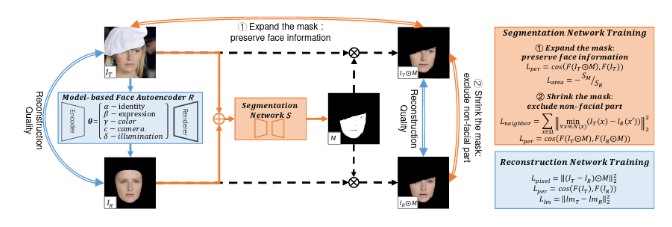
\includegraphics[width=1\linewidth]{focus}
     		 \caption{Chunlu Li és tsai. által javasolt megközelítés felépítése.
     			    Forrás: \cite{focus}}
                    \label{fig:focus}
     	      \end{figure}

            A(z) \ref{fig:focus}. ábrán láthatjuk a $FOCUS$ hálózat felépítését.
            Adott egy $I_{T}$ bemeneti kép, a rekonstrukciós hálózat, $R$, megbecsüli a látens
     	      paramétereket, és ezt követően egy olyan $I_{R}$ képet állít elő, amely csak az
     	      arcot tartalmazza. Ezután az $I_{T}$ és $I_{R}$ képeket betáplálják az 
            $S$ szegmentáló hálózatba, amely megjósolja az $M$ szegmentációs maszkot. A szaggatott vonalak azt mutatják, hogy $M$-et arra használják, hogy az $I_{T}$ és $I_{R}$ képekben a becsült kitakaró tényezőket kiszűrjék a képből, ezáltal összerakott kitakarás mentes képeket kapnak, nevezetesen $I_{T}\bigodot M$ és $I_{R}\bigodot M$ .Megfigyelhetjük, hogy Chunlu Li és tsai. nagy hangsúlyt fektettek a robosztus arcrekonstrukcióra kitakarások mellet. A munkánk szempontjából
     	      azért fontos, mert az arcot kitakaró tényezők mindenütt jelen vannak. 
            Ezért is választottuk a $FOCUS$-t, mert nekik sikerült egy speciális modellt implementálni, ami képes kezelni a kitakarásokat anélkül, hogy szükséges lenne nagy mennyiségű adatra vagy olyan erőforrásra, amihez nincs hozzáférésünk.
     	      A továbbiakban részletesebben megvizsgáljuk a $FOCUS$ építőelemeit és
     	      együttműködésüket.

            Ahogy, már korábban is említve volt, a $FOCUS$ célja 3D-s
     	      arcrekonstrukció egyetlen képből, súlyos kitakarások esetén is. Ezen kihívást
     	      jelentő probléma megoldásához egy modellalapú arc autokódolót, $R$-t és
     	      egy szegmentáló hálózatot, $S$-t implementáltak, ahogyan az a fenti ábrán is
     	      szemléltetve van.
    
            Az arc rekonstrukciójához a szegmentációs maszk a modellillesztés során
     	      kivágja a becsült kitakarásokat, így a rekonstrukciós hálózatot robosztussá
     	      teszi a kitakarásokkal szemben. A szegmentáláshoz a rekonstruált eredmény
     	      referenciaként szolgál, növelve a szegmentálás pontosságát.
    
            Ebben a szakaszban megvizsgáljuk hogyan működik a két hálózat,
     	      hogyan kapcsolódnak egymáshoz, és milyen előnyöket nyújtanak
     	      egymás számára.

            \subsubsection{Modellalapú autoencoder}
        
                A modellalapú arc autokódoló \cite{focus}, $R$, várhatóan rekonstruálja a teljes arc
     	          megjelenését a látható arctartományokból a képen, $I_{T}$-n. 
                Ez egy kódolóból, grafikus renderelőből, és egy dekódolóból áll. A kódoló megbecsüli a látens parmétereket $\theta = [\alpha, \gamma, \phi, c] \in R^{257}$, azaz a 3D alak $\alpha \in R^{144}$, a 3DMM textúrája 
                $\gamma ∈ R^{80}$, a megvilágítás $\phi ∈ R^{27}$, és a jelenet kamera paraméterei $c ∈ R^{6}$. Adott látens parméterekkel a dekódoló a bemeneti képen látható arcképét állítja elő $I_{R} = R(\Theta)$. Majd ehhez egy olyan felügyelet nélküli szegmentáló hálózatot vezetnek be, melynek kimenetelét a modellillesztés során a kitakarások elfedésére lehet használni, és így az autokódolót robosztussá teszi a kitakarásokkal szemben.

            \subsubsection{Szegmentációs hálózat}
    
                A szegmentáló hálózat \cite{focus}, $S$, veszi az $I_{T}$ képet és a szintetizált képet, $I_{R}$-t bemenetként, majd megjósolja a bináris maszkot, $M = S(I_{T} , I_{R}$, annak leírására, hogy egy pixel az arcot ábrázolja-e $(1)$ vagy nem $(0)$. Mivel az $I_R$ tartalmazza a becsült arcot, előzetes tudást biztosít a szegmentáló hálózatnak, és segíti a becslést.
     	
     	          Az arc autokódoló és a szegmentáló hálózat a tanítás során össze 
                vannak kapcsolva olyan módon, hogy egy szinergikus hatást váltanak ki, ami a szegmentálást pontosabbá teszi és a rekonstrukciót robosztussabbá teszi kitakarások jelenlétében.

            \subsubsection{U-Net}
    
                A munkánkban a szegmentáló nagy szerepet játszik, ezért is szeretnénk jobban belemenni a szegmentáló hálózat részleteibe.
    
                Ebben a szekcióban Ronneberger és tsai. \cite{unet} munkája alapján bemutatjuk az U-Net architektúrát, amelyet a saját megvalósításunkban a szegmentációs maszk elkészítésére, optimalizálására használunk fel. 
    
                A konvolúciós hálózatok tipikus felhasználási területe az osztályozási feladatok, ahol a kép kimenete egyetlen osztálycímke. Azonban számos vizuális feladatban, különösen az orvosbiológiai képfeldolgozásban a kívánt kimeneti eredménynek tartalmaznia kell lokalizációt, azaz minden egyes képponthoz osztálycímkét kell rendelni. Továbbá, több ezer tanító kép általában elérhetetlen az orvosbiológiai feladatokban. Ezért Ciresan és tsai. \cite{ciresan} egy csúszóablakos elrendezést alkalmaztak, hogy prediktálják
                az egyes képpontok osztálycímkéjét az adott képpont körüli lokális régió bemenetként történő megadásával.
    
                Ronneberger és tsai. \cite{unet} ezt az architektúrát úgy módosították és bővítették, hogy
                nagyon kevés tanítási képpel működjön, és pontosabb szegmentációkat eredményezzen.
                Az alapötlet a szokásos szűkülő konvolúciós hálózat kiegészítése egymást követő rétegekkel, ahol az összevonó operátorokat felmintavételező operátorok helyettesítik, ezért ezek a rétegek növelik a kimenet felbontását. A lokalizáció érdekében a magas felbontású jellemzőket kombinálják a szűkülő útvonalról származó felskálázott kimenettel. Egy ezt követő konvolúciós réteg ezután megtanulhatja a kimenet precízebb összeállítását ezen információk alapján. A felfelé mintavételezés rész nagyszámú funkciócsatornával is rendelkezik, ami lehetővé teszi a hálózat számára, hogy a kontextusinformációkat továbbítsa a magasabb felbontású rétegek felé. Ennek következtében az expanziós útvonal többé-kevésbé szimmetrikus az összehúzódási útvonalhoz képest és \textbf{U} alakú architektúrát eredményez.
    
                Az UNet egy mélytanulási architektúra, amelyet általában képszegmentálási feladatokhoz használnak. Először 2015-ben mutatta be Olaf Ronneberger, Philipp Fischer és Thomas Brox \cite{unet} az "U-Net: Convolutional Networks for Biomedical Image Segmentation" című tanulmányukban.
    
                Az UNet architektúra egy kódoló és egy dekódoló hálózatból áll. A kódoló hálózat egy sor konvolúciós és összevonó rétegből áll, amelyek lemintavételezik a bemeneti képet, és kivonják belőle a jellemzőket. A dekódoló hálózat felfelé konvolúciós és összekapcsoló rétegek sorozata, amelyek a kép eredeti felbontására felmintavételezik a jellemzőket és szegmentálási maszkot generálnak.
    
                Az UNet architektúrát úgy tervezték, hogy kezelni tudja az osztályok kiegyensúlyozatlanságának problémáját a képszegmentálási feladatokban, ahol az egyes osztályokba tartozó pixelek száma jelentősen változhat. E probléma megoldására az UNet architektúra a kódoló és a dekódoló hálózatok közötti kihagyásos kapcsolatokat használja, amelyek lehetővé teszik a dekódoló számára, hogy a szegmentációs maszk finomításához a kódolótól származó nagy felbontású jellemzőket használja. Az UNet architektúra emellett "vágási" technikát alkalmaz a konvolúciós és összevonó rétegek használatakor fellépő határhatások csökkentésére.
    
                Az UNet architektúrát széles körben használják különböző orvosi képalkotó alkalmazásokban, mint például a tumorok felismerése, az agy szegmentálása, és a sejtek szegmentálása. Más területeken is  alkalmazták, például a természetes jelenetek szegmentálásában, ahol ígéretes eredményeket mutatott.
    
                A hálózat felépítését a(z) \ref{fig:unet}. ábra szemlélteti. A rendszer egy szűkülő (bal oldal) és egy bővülő útvonalból (jobb oldal) áll. Az összehúzódó útvonal a konvolúciós hálózatok tipikus architektúráját követi. Ez a következő lépések ismételt meghívásából áll: 
                két 3x3-as konvolúció, melyeket egy-egy ReLU és egy 2x2 max pooling művelet követ. Minden lefelé mintavételezést a jellemzőcsatornák duplázása követ. 
    
                Az expanzív útvonal minden lépése a jellemzőtérkép felmintavételezéséből áll, amelyet egy 2x2-es konvolúció követ, amely megfelezi a jellemzőcsatornák számát, majd egy konkatenáció a megfelelően levágott jellemzőtérképpel a kontraháló útvonalról, és két 3x3-as konvolúció, amelyet egy-egy ReLU követ. A vágásra a határpixelek elvesztése miatt van szükség minden egyes konvolúcióban. Az utolsó rétegben egy 1x1-es konvolúciót használnak minden egyes 64 komponensű jellemzővektor a kívánt számú osztályhoz való kötéséhez. Összességében a hálózat 23 konvolúciós rétegből áll.
    
                Tehát, az UNet egy nagy teljesítményű mélytanulási architektúra, amelyet gyakran használnak képszegmentálási feladatokra, különösen az orvosi képalkotás területén. 
        
                \begin{figure}[h]	
     	              \centering
     	        	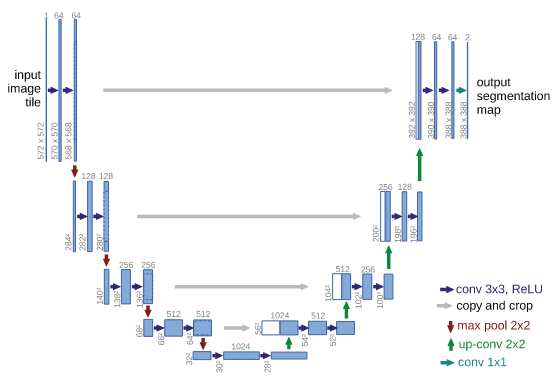
\includegraphics[width=0.7\linewidth]{unet}
     	        	\caption{U-Net felépítése
     	        		Forrás: \cite{unet}}
                    \label{fig:unet}
     	        \end{figure}
              \clearpage
 	
            \subsubsection{Tanítás}
            
         	      Az arc autokódoló és a szegmentáló hálózat kölcsönös függőségei miatt 
                egy \textit{Expectation − Maximization (EM)} típusú stratégiát alkalmaztak,
         	      ahol a két hálózatot váltakozva tanították be. Ez lehetővé tette a stabil
         	      konvergenciát a betanítási folyamat során. Mint más EM típusú tanítási
         	      stratégiákhoz hasonlóan, a tanítási folyamatuk a modell paraméterinek
         	      durva inicializálásával kezdődik, amely felügyelet nélküli módon történik.
         	
         	      A szegmentáló hálózat tanításakor az arc autokódoló paraméterei
         	      rögzítettek és csak a szegmentáló hálózatot optimalizálják. Alapvetően 
                négy költségfüggvényt javasolnak, amelyek kikényszerítik a képek közötti hansolóságokat. A költségfüggvények dolga hogy, eldöntse egy adott pixelről hogy az arc része vagy sem. Ezek perceptuális szinten vagy pixel szinten dolgoznak, hogy teljes mértékben kihasználják a vizuális nyomokat.
         	
         	      Betanítás során a szegmentáló hálózat feladata, hogy egyensúlyt
         	      keressen az olyan képpontok elvetése között, amelyeket az autokódoló nem
         	      tud jól értelmezni és az olyan képpontok megőrzése között, amelyek fontosak
         	      a bemeneti kép és az előállított arc perceptuális reprezentációjának 
                megőrzése érdekében. Ezáltal nincsen szükség a kitakarások felügyeletére.
         	
         	      Az autkódoló betanítása során tovább optimalizálták a kódoló paramétereit, 
                közben a szegmentáló hálózat rögzítve van. Az autokódolóhoz az alábbi költségfüggvények tartoznak:
        
                \begin{equation*}
                    L_{pixel} = \parallel (I_{T} − I_{R}) \bigodot M \parallel _{2}^{2} 
                \end{equation*}
                
                \begin{equation*}
                    L_{per} = \cos(F(I_{T}), F(I_{R}))    
                \end{equation*}
                
                \begin{equation*}
                    L_{lm} = \parallel lm_{T} - lm_{R} \parallel _{2}^{2}  
                \end{equation*}
            \subsubsection{Adathalmazok}
            
             	Az általuk felhasznált adatbázisok a CelebA-HQ és az AR adathalmaz.
             	Ezek segítségével értékelik az illesztés és az arcszegmentlás hatékonyságát.
             	Az alakrekonstrukció kiértékelésére a NoW adatbázis
             	részhalmazait használták (\ref{fig:now}. ábra).
     	
             	\begin{figure}[h!]	
             		\centering
             		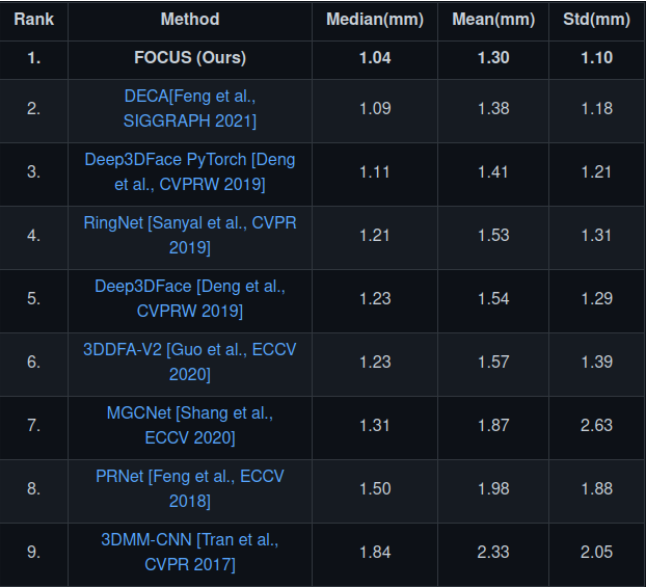
\includegraphics[width=0.7\linewidth]{now}
             		\caption{NoW Challenge benchmark eredményei
             			Forrás: \url{https://github.com/unibas-gravis/Occlusion-Robust-MoFA}}
                    \label{fig:now}
             	\end{figure} 

              \newpage
              
        \subsection{Renderelés}

            A renderelés mind a FOCUS \cite{focus}, mind a DECA \cite{deca} projektben fontos, mivel lehetővé teszi a neurális hálózati modellek tanításához szükséges valósághű szintetikus képek létrehozását, valamint a 3D-s tárgyak vagy animált arcok valósághű vizuális reprezentációjának előállítását. A renderelés minősége mindkét projektben jelentős hatással van a végső kimenet pontosságára és valósághűségére.

            Mi ebben a fejezetben inkább Yao Feng és tsai. \cite{deca} által ajánlott módszert vizsgáljuk meg jobban, mivel a mi munkánk arcrekonstrukciós hálózata az ő munkájukon alapszik.

            A DECA projekt szempontjából a renderelés azért fontos, mert ez az utolsó lépés az arc rekonstrukciós folyamatában, amely az animált arc valósághű 2D-s képét állítja elő.

            A rendszer az arc időbeli mozgását és deformációját egy mély neurális hálózati modell segítségével rögzíti, amely a bemeneti képek vagy videoképek alapján megjósolja egy 3D-s arcmodell paramétereit. Maga a 3D arcmodell azonban nem közvetlenül megfigyelhető, ezért 2D-s képpé kell renderelni, hogy az arcanimáció vizuális megjelenítése létrejöjjön.
            
            A renderelés minősége jelentős hatással van a végeredmény realizmusára és hihetőségére. Egy kiváló minőségű renderelőmotor képes valósághű fény- és árnyékhatásokat, pontos bőrszínt és sima mozgást produkálni, amelyek mind hozzájárulnak az animált arc általános vizuális hűségéhez.
            
            A DECA-ban használt differenciálható renderelő továbbá lehetővé teszi a renderelt képek vagy videóképek gradiensének kiszámítását a bemeneti 3D geometria és más renderelési paraméterek tekintetében, lehetővé téve az arc teljesítményének rögzítéséhez használt neurális hálózati modellek végponttól végpontig tartó tanítását.

            \subsubsection{Differenciálható renderelő}

                A differenciálható renderelő a DECA projekt kulcsfontosságú eleme. A korábban említettek alapján láthajuk, hogy fontos szerepe van.

                 Ebben a fejezetben Kato és tsai. \cite{diffrenderer} kutatása alapján bemutatjuk a differenciálható renderelő alapelvét.

                A legtöbb 3D becslési módszer a felügyelt tanítási rendszerekre és költséges címkézésekre támaszkodnak, ami
                a 3D megfigyelések összes paraméterének összegyűjtését jelentősen megnehezíti. A megközelítések egyike a grafikus renderelési folyamatok integrálása a neurális hálózattal működő rendszerekbe. Ez lehetővé teszi az átalakítást és a 3D becslések beépítését a 2D képi szintű információkba.

                A differenciálható renderelés (DR) olyan technikák családját alkotja, amelyek a renderelési folyamat hasznos gradienseinek kinyerésével végponttól-végpontig tartó optimalizálás céljából integrációt valósítanak meg. A renderelés differenciálásával a DR áthidalja a szakadékot
                a 2D és a 3D feldolgozási módszerek között, lehetővé téve a neurális hálózatok számára, hogy 2D-s vetületeken dolgozva optimalizálják a 3D-s entitásokat. Amint a(z) \ref{fig:diffrenderer}. ábrán látható, a 3D jelenet paramétereinek optimalizálása a gradiensek visszaterjedésével érhető el a renderelési kimenethez képest. 

                Az általános 3D önfelügyeleti modell a renderelő réteg integrálásával a megjósolt jelenetparaméterekhez és a veszteség alkalmazásával a renderelt és a bemeneti kép különböző módokon történő összehasonlításával történik.

                \begin{figure}[h!]	
            		\centering
            		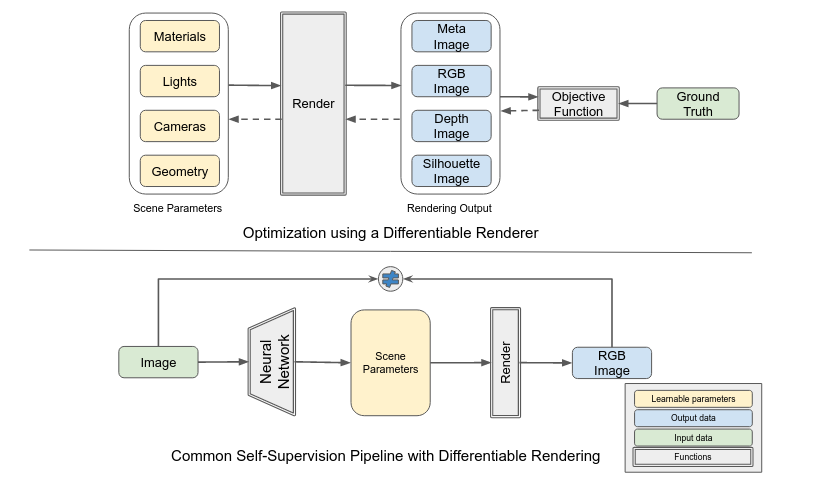
\includegraphics[width=1\linewidth]{diffrenderer}
            		\caption{Általános önfelügyeleti modell differenciálható rendereléssel.\\
                            Forrás: \cite{diffrenderer}}
                    \label{fig:diffrenderer}
            	\end{figure}

                A DECA-ban a differenciálható renderelőt a renderelt arcképek vagy videóképek gradiensének kiszámítására használják a 3D arcgeometria és más modellparaméterek tekintetében. Ez lehetővé teszi a hiba-visszaterjesztést és más gradiens-alapú optimalizálási technikák használatát az arc teljesítményének teljes körű rögzítésére szolgáló neurális hálózati modellek betanításához.

                A tanítás során a differenciálható renderelőt szintetikus arcképek egy sorának renderelésére használják a 3D arcmodellek és a megfelelő kifejezések véletlenszerűen generált készletének felhasználásával. A renderelt képeket ezután egy veszteségfüggvény segítségével összehasonlítják egy alapigazság képkészlettel. A veszteségfüggvény gradienseit a 3D arcmodellek és más modellparaméterek tekintetében a differenciálható renderelő segítségével számítják ki és a modellsúlyok frissítésére használják.
                
                A differenciálható renderelő ilyen módon történő használatával a DECA képes olyan neurális hálózati modelleket tanítani, amelyek képesek megragadni az arckifejezések és a mögöttes 3D arcgeometria közötti összetett kapcsolatot és kiváló minőségű arcanimációkat készíteni a bemeneti képekből.

            \subsubsection{Raszterizáló}

                A DECA projekt keretében a raszterizáló a renderelési folyamat utolsó lépésében játszik szerepet, amely a 3D arcmodell 2D képpé vagy videoképpé alakítása. A raszterizáló felelős a 3D arcmodell 2D-s képsíkra történő vetítéséért.

                A raszterizáló a grafikus folyamat egyik összetevője, amelyet a számítógépes grafikában és a játékfejlesztésben gyakran használnak. Úgy működik \cite{standard-rasterizer}, hogy az archáló csúcsainak 3D-s koordinátáit egy 2D-s képsíkra vetíti. A vetítés során a 3D koordinátákat 2D képernyőkoordinátákká alakítják át figyelembe véve a kamera perspektíváját és minden egyéb releváns paramétert, például a látómezőt és a képarányt.
                
                Miután az arc hálójának csúcsait kivetítették a 2D-s képsíkra, a raszterizáló a hálót alkotó háromszögeket kitölti a megfelelő színekkel vagy textúrainformációkkal a renderelési folyamat során korábban elvégzett megvilágítási és árnyékolási számítások alapján.
                
                A raszterizáló kimenete egy pixelalapú kép vagy videókép, amely a renderelt 3D arcanimáció részleteit rögzíti.

            \subsubsection{Renderelési folyamat}

                A renderelési folyamat a DECA alapján több lépésre bontható:

                \begin{enumerate}
                    \item \textbf{Az arc tájékozódási pontjainak felismerése}: A rendszer először az arc tájékozódási pontjait észleli a bemeneti képeken vagy videóképeken. 

                    \item \textbf{Kép normalizálás}: A bemeneti képeket vagy videoképeket szabványos méretre és felbontásra normalizálják.

                    \item \textbf{3D arc rekonstrukció}: A DECA az észlelt arctájékozódási pontjainak felhasználásával rekonstruálja az arc 3D-s modelljét. A 3D modell csúcspontokból álló hálóból áll, amelyek a 3D térben úgy helyezkednek el, hogy megfeleljenek az arc alakjának és kontúrjainak.

                    \item \textbf{Textúra leképezés}: A 3D arc rekonstrukció után a rendszer textúratérképet alkalmaz a 3D arcmodellre, hogy valósághű bőrszínt és részleteket adjon hozzá.

                    \item \textbf{Világítás és árnyékolás}: A 3D arcmmodellre világítást és árnyékolást alkalmaznak, hogy valósághű fénypontokat és árnyékokat hozzon létre. 

                    \item \textbf{Renderelés}: Végül a DECA rendereli a 3D arcmodellt az alkalmazott textúrával, világítással és árnyékolással, hogy az animált arcról valósághű 2D képet készítsen.
                    
                \end{enumerate}

            \subsection{Arcpontok felismerése} \label{FAN}

            A valósághű 3D arcrekonstrukció elérése érdekében fontos, hogy az adatokat előkészítsük még a tanítási folyamat előtt. Ez a lépés a munkánkban az arc jellegzetes pontjainak detektálását, majd a pontok \textit{.csv} fáljokba való kiírását jelenti. Yao Feng és tsai. \cite{deca} megközelítését követve Bulat és tsai. \cite{bulat} FAN modelljét használjuk a 68 db 2D-s jellegzetes pont (landmark) detektálásához. A FAN egy arcpontok lokalizálására szolgáló reziduális hálózaton alapuló architektúra, amelyet  egy nagy, de szintetikusan kibővített 2D-s arcpont-adathalmazon tanítottak. Ezután 5 adathalmazon, nagyjából 230 000 képpel értékelték ki a hálózatot és átlagosan 68,36\%-os pontosságot értek el.

            A FAN modell Python-csomagként megtalálható \textit{face-alignment} néven, amely egy olyan eszközkészletet biztosít, amely az arc tájékozódási pontjainak felismerésére, a fej pózának becslésére és az arc igazítására szolgál. 
            Mély tanulási modelleken alapul, és az arcképek előfeldolgozására használható olyan feladatok elvégzése előtt, mint az arcfelismerés vagy az érzelemérzékelés.
            
            A csomag több modulból áll, amelyek mindegyike az arcelemzéssel kapcsolatos speciális feladatot lát el. Az egyes modulok:

            \begin{itemize}
                \item \textbf{észlelés}:  Ez a modul SSD (Single Shot Detector) architektúrán alapul és előre betanított modelleket használó arcfelismerő funkciókat biztosít. Az arcdetektor betanítható az arcok felismerésére különböző beállítások mellett, például gyenge fényviszonyok, eltakart arcok vagy profilnézet esetén.
        
                \item \textbf{igazítás}: Ez a modul funkciókat biztosít az arc tájékozódási pontjainak felismeréséhez és az arcok igazításához.
        		A tájékozódási pont detektor egy mély konvolúciós neurális hálózatot (CNN) használ az arc kulcsfontosságú pontjainak, például a szemeknek, az orrnak és a szájnak a helyzetének a felismerésére. 
        		Az arcigazítási funkció ezután a tájékozódási pontok pozícióit használja fel az arckép geometriai transzformációjának elvégzéséhez.
        
                \newpage
                \item \textbf{póz}: Ez a modul funkciókat biztosít az arc fejpózának becslésére, ami a fej kamerához viszonyított orientációját jelenti. A pózbecslő egy CNN-t használ a fej gördülési és dőlési szögének becslésére.
                
                \item \textbf{segédeszközök}: Ez a modul egy sor segédfunkciót biztosít a képfeldolgozáshoz, mint például a méretváltoztatás, a képkivágás és a színnormalizálás.
        
            \end{itemize}
 	      \subsection{Értékelés}

            Mint láthatjuk a fent említett megközelítések mind kiváló eredményeket nyújtanak, de megfigyelhetjük hogy a két munkának a szerzői teljesen különböző motivációval rendelkeztek.
            
         	A $DECA$ főbb motivációja az emberi arc részleteinek megőrzése valamint az arc realisztikus animálhatósága. A $FOCUS$ célja pedig egy gyors modell kialakítása volt, amely korábbi munkákhoz képest jobban kezeli a kitakarásokat. A mi célunk, egy olyan animálható modell kialakítása, amely képes megőrízni a részleteket, emellett képes konzisztens mükődést nyújtani súlyos kitakarások jelenlétében is.
 	
 	          Tehát a tervezett modell, amit a későbbiekben részletesebben
 	          megvizsgálunk kettő egymást támogató hálózatból áll. Egyik fő 
            épitőeleme a $DECA$ alapján készített rekonstrukciós hálózat, másik a $FOCUS$ megközelítésében implementált szegmentációs hálózat. E két hálózaton egy EM típusú stratégiát alkalmazunk a tanítási folyamat során.


    \section{A tervezés során végzett munkafázisok}

        \subsection{Adathalmazok kiválasztása}

        Az adathalmaz kiválasztása rendkívül fontos az eredmény minősége szempontjából. Az egyik cél az arcrekonstrukciós hálózat felépítépítése, ezért szükséges olyan adathalmazok kiválasztása, amelyek nagy mennyiségű arcképet tartalmaznak. Az adathalmazokat olyan forrásokból szükséges kiválasztani, amelyek megbízhatóak és széles körben használtak, mint például a CelebA, LFW, vagy az Imagenet adathalmazok. Az adathalmazoknak tartalmaznia kell arcképeket több különböző pozícióban, háttérrel és fényviszonyokkal, hogy a hálózatunk jól teljesítsen különböző körülmények között.

        Az adathalmaz kiválasztása az érzelmi állapot felismeréséhez fontos szerepet játszik, mivel az adathalmaz minősége hatással van a modell teljesítményére. A feladat az, hogy az arcképek alapján az érzelmi állapotot felismerjük, és a nemet is megállapítsuk. Ennek érdekében olyan adathalmazokat kell kiválasztanunk, amelyek tartalmaznak arcképeket mind férfiakról, mind nőkről, és amelyek különböző érzelmi állapotokat képviselnek.

        Az érzelmi állapotok felismerésére a legmegfelelőbb adathalmazok a különböző színészek, énekesek vagy sportolók képeit tartalmazó adatbázisok, mint például a FER-2013 vagy a FERPlus adathalmaz. Ezek az adathalmazok tartalmaznak olyan arcképeket, amelyekhez címkéket is mellékeltek, azaz az érzelmi állapotot is jelölték, így a modellünk számára egyszerűbb lesz az érzelmek felismerése. Ezen adathalmazok kiválasztásakor fontos figyelembe venni az adatok minőségét, mennyiségét, valamint a felhasználói licencet.

        Az adathalmazban szükséges biztosítani a nemek arányos eloszlását is, amely lehetővé teszi a modell számára, hogy hatékonyan dolgozzon a férfiak és a nők arcképeivel egyaránt. Az adathalmaznak tartalmaznia kell olyan arcképeket, amelyek széles körű különbségeket mutatnak a férfiak és nők fizikai jellemzői között, például az arc formájában, valamint a szemek és az ajkak méretében. Ennek érdekében ajánlott olyan adatbázisokat választani, amelyek tartalmaznak arcképeket mindkét nemről.

        Az adathalmaz összeállítása előtt érdemes alaposan megvizsgálni az adatbázis forrásait, és bizonyosodni arról, hogy az adatok jogosultak-e a felhasználásra. A privát adatokat tartalmazó adatbázisokat el kell kerülni, és olyan adatokat kell választani, amelyek nyilvánosan elérhetők, és szabadon felhasználhatók.
        
        \subsection{Keretrendszer kiválasztása}

        Az arcrekonstrukciós hálózat és az arcanalízis hálózat tervezése során fontos szempont a technológia kiválasztása, amely lehetővé teszi a modellünk hatékony és megbízható működését. A pytorch, tensorflow és keras az elmúlt években az iparágban elterjedt neurális hálózat keretrendszerek, amelyek mindegyike képes a nagy számítási teljesítményű modellek létrehozására és azok hatékony működtetésére.

        A pytorch keretrendszer mellett döntöttünk, mert az egyik legelterjedtebb és legnépszerűbb keretrendszer a neurális hálózatok számára. Az erőteljes számítási és automatizálási funkciói, valamint az egyszerű, de hatékony programozási nyelve miatt kiváló választásnak bizonyult. A pytorch átfogó dokumentációja és a közösség által készített rengeteg mintakód is segít abban, hogy könnyedén megértsük a keretrendszer működését és az algoritmusokat.
        
        \subsection{Meglévő munkák megvizsgálása}

        Az hálózatok építése előtt érdemes megvizsgálni azokat a kutatási eredményeket, amelyek már elkészültek ezen területeken. Ezek az eredmények felhasználhatóak lehetnek a hálózatunk tervezéséhez, vagy javaslatot tehetnek azokra a paraméterekre, amelyeket érdemes beállítani. Érdemes áttekinteni az összes fontos kutatási eredményt, és kiválasztani azokat, amelyek a legjobban illeszkednek a projektre.
        
        \subsection{Tapasztalatok}

        Az arcrekonstrukciós hálózat és az arcanalizáló hálózat fejlesztése egy olyan új terület, amelyet a csapatunk még nem tapasztalt korábban. Ennek eredményeképpen sok időt kellett szánnunk az anyag megértésére és a szükséges ismeretek megszerzésére.

        A publikus adathalmazok száma viszonylag alacsony volt, ami további nehézséget jelentett a fejlesztési folyamat során.
        
        A fejlesztői környezet sok komponensből áll, és sokuk nem natív windowson. Ez kihívást jelentett a fejlesztés során, mivel a csapatunk Windows operációs rendszert használt. Ennek ellenére megoldást találtunk a problémákra, és sikerült sikeresen felépítenünk a hálózatokat.
    
    \section{Megvalósítás}
    
        Ebben a fejezetben a projektünk redszertervét, arcanalízis- és arcrekonstukció felépítését, valamint kulcsfontosságú metódusait mutatjuk be részletesen.
        
        \subsection{Felhő alapú architektúra}
        
            Ebben a projektben több mikroszervizt készítettünk, amelyek együttműködnek, hogy egy teljes alkalmazást hozzanak létre az arc rekonstrukciójára és elemzésére. A mikroszolgáltatások közé tartozik egy Java backend, egy React.js frontend és két Python modul az arcrekonstrukciós modellünkhöz és az arcelemző modellünkhöz.

            A Java backend felelős az adattárolásért és a többi mikroszolgáltatással való
            API-kommunikációért. A React.js frontend egy felhasználóbarát felületet biztosít a felhasználók számára az alkalmazással való interakcióhoz, valamint a rekonstruált arcok és az elemzési eredmények megjelenítéséhez. A Python modulok tartalmazzák az arcok rekonstrukciójához és elemzéséhez szükséges gépi tanulási modelleket, és kommunikálnak a Java backenddel a bemenet fogadásához és a kimenet biztosításához.

            Annak érdekében, hogy a mikroszolgáltatások skálázhatóak, megbízhatóak és karbantarthatóak legyenek egy helyi Kubernetes klaszterre telepítjük őket a minikube segítségével. A Kubernetes egy nyílt forráskódú platform a konténer-orchestráláshoz, amely lehetővé teszi számunkra a konténeres alkalmazások kezelését, telepítését és skálázását. A minikube viszont egy olyan eszköz, amely lehetővé teszi a fejlesztők számára, hogy a Kubernetes-t lokálisan futtassák a gépeiken.

            A projekt egyik célja, hogy bemutassuk a mikroszerviz architektúra előnyeit, valamint a jobb skálázhatóság, hibatűrés és rugalmasság érdekében a Kubernetes klaszterre való telepítés fontosságát. Különböző Kubernetes fogalmakat is meg fogunk vizsgálni, mint például a podok, szolgáltatások, telepítések és skálázás, hogy biztosítsuk a mikroszolgáltatások zökkenőmentes működését a klaszteren. A projekt végére jobban megértjük majd, hogyan működnek a mikroszolgáltatások, és hogyan telepíthetjük őket egy Kubernetes klaszterre a minikube segítségével, miközben egy funkcionális alkalmazást készítünk az arcok rekonstrukciójára és elemzésére.

            \begin{figure}[h]	
        		\centering
        		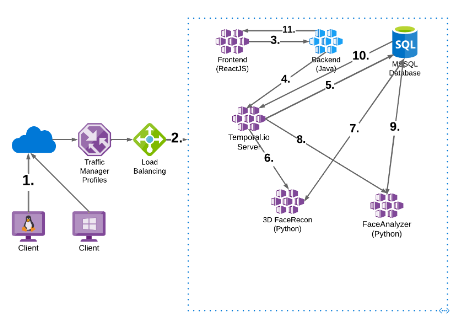
\includegraphics[width=0.7\linewidth]{sysplan}
        		\caption{ A rendszer felépítése}
        	    \label{fig:sysplan}
            \end{figure}

            \clearpage

        	Továbbiakban megvizsgáljuk a rendszer felépítését illetve mükődését a
        	fenti ábra segítségével. A(z) \ref{fig:sysplan}. ábrán látható, hogy 6 különböző szolgáltatást Minikube lokális klaszteren üzemeltetünk.

        	A 6 különböző szolgáltatás az alábbiak:
        	\begin{itemize}
        		\item Frontend
        		\item Backend
        		\item Temporal.io szerver
        		\item 3D arcrekonstrukciós modul
        		\item Arcanalízis modul
        		\item Adatbázis
        	\end{itemize}
        
        	Ha megnézzük a fenti ábrát, láthatjuk hogy, a workflow belépési pontja a HTTP kérés, aminek payload-ja, a kép egy célszemélyről, és amint a
        	frontend-től megkapja a kérést a backend, az elindítja a workflow-t. A következő lépés hogy, a workflow metódusai egymás után meghívódnak.
        	Végül a felhasználó visszakapja a rekonstruált képet, illetve a képen lévő személy akkori érzelmi állapotát és nemét. Az arcrekonstrukciós és arc analízis moduljainkat Python nyelven implementáltuk, mivel mesterséges intelligenciával dolgozunk, a különböző nagymennyiségű Python könyvtár elérhetősége nagy mértékben megsegítette munkánkat.
        
        \subsection{Frontend}

            A frontend egy webalapú felhasználói felület, amely a React.js, a felhasználói felületek készítésére szolgáló népszerű JavaScript-könyvtár segítségével készült.

            A frontend alkalmazás fő összetevői közé tartozik egy fájlfeltöltő komponens és egy eredménykomponens. A fájlfeltöltő komponens lehetővé teszi a felhasználók számára, hogy képfájlt válasszanak ki a számítógépükről vagy eszközükről. Az eredménykomponens megjeleníti az arcfelismerési és elemzési eredményeket, tehát a nemet, az érzelmeket és a rekonstruált 3D képet.

            A konténerizáció során megcsináltuk a szükséges Dockerfile-t. A Dockerfile tartalmazza a szükséges csomagok vagy könyvtárak telepítésére, az alkalmazás kódjának a konténerbe történő másolására, valamint az alkalmazás futtatásához szükséges parancs megadására vonatkozó utasításokat. 

            Miután a Docker konténer elkészült, létrehoztuk a Kubernetes telepítési fájlokat, amelyek meghatározzák, hogyan kell a konténereket telepíteni és kezelni, majd a konténer telepíthető a Minikube klaszterre.
            
        \subsection{Backend}

            A Backend egy Spring Boot Java implementáció amely felelő az adattárolásért és a többi mikroszolgáltatással való API-kommunikációért.

            A Spring Boot egy népszerű Java-alapú keretrendszer, amely egyszerűsített módot biztosít a webes alkalmazások építésére és futtatására. Számos alapfunkciót kínál, például automatikus konfigurációt, beágyazott kiszolgálókat és biztonságot, ami ideális választássá teszi a mikroszolgáltatások építéséhez.
            
            A Temporal.io egy olyan technológia, amely segítségével gyorsan és
        	egyszerűen tudunk workflow-t implementálni. Ehhez szükséges a szerver,
        	mert ott bonyolódik le egy workflow sikeres elvégzése, vagy hiba esetén
        	biztosít egy dashboard-ot, amivel megtudjuk vizsgálni a hiba okát. 

            Ebben a projektben a Gradle-t használtuk a függőségek kezeléséhez és az alkalmazás készítéséhez. A Temporal.io SDK-t is beépítettük a Spring Boot alkalmazásunkba a munkafolyamat megvalósításához.

            A munkafolyamatban a elöszőr elmentjük a képet az adatbázisba, majd a képről generáltatunk egy 3D-s rekonstrukciót, ezután az arcanalízis modul segítségével megkapjuk a képen lévő személy érzelmi állapotát illetve nemét.

            A konténerizáció folyamata hasonlóan van implementálva mint a frontend esetében.
         
        \subsection{Adatbázis}
            A projektünk MongoDB Atlas-t használ adatbázisként.

            A MongoDB Atlas használatával a projekt egy nagy rendelkezésre állású és skálázható adatbázis-megoldás előnyeit élvezheti, olyan funkciókkal, mint az automatikus biztonsági mentések, a több régióra kiterjedő klaszterek és a végponttól végpontig titkosítás. Az adatbázis könnyen kezelhető a webalapú Atlas felhasználói felület vagy az átfogó API segítségével. 
            
            Ez azért volt számunkra előnyös, mert nekünk csak az alkalmazás logikájának kialakítására kellett koncentrálnunk anélkül, hogy az adatbázis infrastruktúrájával kellene foglalkoznunk.

            Összességében a MongoDB Atlas-t használó projekt képes kihasználni a dokumentumalapú adatbázis erejét és rugalmasságát, miközben egy felhőalapú menedzselt szolgáltatás előnyeit is élvezné.

            Az adatbázisban eltároljuk a képet, illetve a szükséges adatokat hogy a későbbiekben megtudjuk jeleníteni a szükséges adatokat.
            
        \subsection{Arcanalízis}

            Az arckifejezés-felismerés és a nemek osztályozása a számítógépes látás két fontos feladata, amelyeknek számos alkalmazása van, például az ember-számítógép interakció, a biztonság és a szórakoztatás területén. Ebben a projektben célunk különböző mélytanulási modellek implementálása és összehasonlítása mind az arckifejezés-felismeréshez, mind a nemek osztályozásához a népszerű arcfelismerési adathalmazok, például a FER-2013 adathalmaz felhasználásával. Különböző architektúrákat fogunk vizsgálni, például a konvolúciós neurális hálózatokat (CNN) és előre betanított modelleket, például a ResNet-et, hogy olyan modelleket építsünk, amelyek pontosan felismerik az arckifejezéseket és osztályozzák a képen szereplő személy nemét. Az egyes modellek teljesítményét is értékelni fogjuk. A projekt eredménye hasznos lehet különböző valós alkalmazásokban, például az érzelmek felismerésében a szociális robotikában, a megfigyelőrendszerekben és a személyre szabott reklámokban.
        
            \subsubsection{Adathalmazok}
                Az arc kifejezések klasszifikációjához a FER-2013 adathalmazt használjuk \url{https://www.kaggle.com/datasets/msambare/fer2013}. Az adatok 48x48 pixeles, szürkeárnyalatos arcképekből állnak. Az arcokat automatikusan úgy regisztrálták, hogy az arc többé-kevésbé középen legyen, és minden képen körülbelül ugyanannyi helyet foglaljon el.
                
                A feladat az egyes arcok kategorizálása az arckifejezésben megjelenő érzelem alapján a hét kategória egyikébe (0=dühös, 1=undor, 2=félelem, 3=boldog, 4=szomorú, 5=meglepetés, 6=semleges). A tanítóhalmaz 28 709 példából, a nyilvános teszthalmaz pedig 7178 példából áll.
                
                \begin{table}[h]
                    \begin{tabular}{lll}
                        Érzelmek    & \begin{tabular}[c]{@{}l@{}}Darabszám\\ (Tanítás)\end{tabular} & \begin{tabular}[c]{@{}l@{}}Darabszám\\ (Tesztelés)\end{tabular} \\
                        semleges    & 4965                                                          & 1233                                                            \\
                        meglepődött & 3171                                                          & 831                                                             \\
                        undor       & 436                                                           & 111                                                             \\
                        boldogság   & 7215                                                          & 1774                                                            \\
                        félelem     & 4097                                                          & 1024                                                            \\
                        szomorúság  & 4830                                                          & 1247                                                            \\
                        mérges      & 3995                                                          & 958                                                            
                    \end{tabular}
                    \caption{A adathalmaz felosztása a tanításhoz}
                \end{table}
                    
                
                A nemek osztályozásához a $Kaggle$ – $Gender$ $Classification$ $Dataset$-et használtuk fel \url{https://www.kaggle.com/datasets/cashutosh/gender-classification-dataset}. Az adathalmaz nagyjából $23 200$ női és $23 800$ férfi arc megtisztított és levágott képeit tartalmazza.
            \subsubsection{Adatok előkészítése}

                Az arcanalízis rendszerünk tanításához az első lépcsőfokunk a képek pixelértékeit az adathalmaz átlagához és szórásához viszonyítva normalizálni. A második lépés a megfelelő transzformációkat elvégezni a képeken.

            \subsubsection{Tanítás}
                
                    Az arcanalízis két különböző hálózatból épül fel. Az egyik hálózat hét alapvető arckifejezés felismeréséért felel, a másik pedig a nemek klasszifikálásáért,
                    melyek mind előre tanított ResNet-18 háló továbbtanításán alapszanak.
                    A hálózatok utolsó rétege egy-egy teljesen összekapcsolt réteg.
                    A hálózatok tanítása során SGD optimalizálót használunk és bináris-, többkategóriás keresztentrópia költségfüggvényekkel mérjük a modellek teljesítményét.

                    A tanítás folyamata az alábbi: 
                        \begin{enumerate}
                            \item A szkript a szükséges könyvtárak importálásával és a modell néhány hiperparaméterének, például a tanulási ráta meghatározásával kezdődik.

                            \item Ezután betölti a tanítási adatokat, és feldolgozza azokat néhány képi augmentációs technikával, például véletlenszerű forgatással és átfordítással. A kiterjesztett adatokat ezután tanítási és validálási halmazokra osztja.

                            \item A modell inicializálása a ResNet18 architektúrával történik, az utolsó rétegek némi módosításával, hogy a nemek osztályozásánál bináris, míg az érzelmek felismerésénél többkategóriás osztályozást adjon ki. 

                            \item Meghatározza a modell veszteségfüggvényét, amely a bináris kereszt-entrópia függvény. Beállítja az optimalizálót is, amely sztochasztikus gradiens ereszkedést (SGD) használ momentummal.

                            \item Megkezdődik a tanítási ciklus, ahol a modellt egy megadott számú epochán keresztül képezzük. A szkript minden egyes ciklus esetében kötegenként végighalad a tanítási készleten, hiba-visszaterjesztés segítségével kiszámítja a veszteséget és a gradienseket, és az optimalizáló segítségével frissíti a modell súlyait.

                            \item Minden egyes ciklus után kiszámítja a pontosságot és a veszteséget a validációs készleten.

                            \item Végül a betanított modell elmentésével zárul a folyamat.
                        \end{enumerate}\\

                    Tanítás során az alábbi hiperparamétereket használtunk:
                        \begin{itemize}
                            \item a tanulási ráta: $0.0009$ 
                            \item a momentum: $0.9$
                            \item a ciklusok száma : $7$
                        \end{itemize}
        \subsubsection{Tanítási környezet}

        Az érzelemfelismerő és a nemfelismerő hálózatokat Intel(R) Core(TM) i5-7600K CPU @ 3.80GHz processzorral, 16,0 GB DDR4 RAM és NVIDIA GeForce GTX 1660 SUPER 6GB videókáryával rendelkező számítógépen tanítottuk, illetve fejlesztettük.
                    
                        
        \subsection{Arcrekonstrukció}
            \subsubsection{Adathalmazok}
                
                A rekonstrukciós modellünk a nyilvánosan elérhető CELEBA \cite{celeba} adathalmazból tanul. A $CelebFaces Attributes Dataset$ (CelebA) egy nagyméretű arcattribútum adatkészlet, amely több mint 200 000 híresség képét tartalmazza, mindegyikhez 40 attribútum annotáció tartozik. Az adatállomány képei nagy pózvariációkat és háttérzavarokat fednek le. A CelebA nagy változatossággal, nagy mennyiségben és gazdag annotációkkal rendelkezik, többek között az alábbiakkal:

                \begin{itemize}
                    \item 10 177 különböző személyazonosság
                    \item 202 599 darab arckép
                    \item 5 jellegzetes arcpont, képenként 40 bináris attribútum annotációja
                \end{itemize}

                A CelebA adathalmaz részhalmazokra törénő felbontását a(z) \ref{fig:celeba-sets}. táblázat szemlélteti.
            
                \begin{table}[h]
                    \centering\begin{tabular}{lll}
                    Adathalmaz    & \begin{tabular}[c]{@{}l@{}}Darabszám\end{tabular}\\
                    tanuló    & 162770                                                           \\
                    validációs & 19962                                                           \\
                    teszt       & 19868                    
                    \end{tabular}
                    \caption{CelebA adathalmaz felbontása részhalmazokra.}
                    \label{fig:celeba-sets}
                \end{table}
            
            \subsubsection{Arcrekonstrukciós hálózat adatainak előkészítése}

            A \textit{list\_eval\_partition.csv} megadja, hogy az adott kép melyik adathalmazhoz tartozik.
           A három adathalmaz a tanító, a tesztelési és a validációs halmazok. A(z) \ref{FAN} fejezetben említett FAN modellt felhasználva detektáljuk képenként a 68 db arcpontot, majd azok mentésre kerülnek a kép partíciójának megfelelő .csv fájlba. A .csv fájlok a \textit{train\_landmarks.csv}, \textit{test\_landmarks.csv} és a \textit{val\_landmarks.csv}.

            \subsubsection{Szegmentáló hálózat adatainak előkészítése}

             A szegmentáló hálózat súlyainak durva inicializálása érdekében a hálózatot elő kell tanítanunk. A hálózat (U-Net) előtanításához adatokat kell generálnunk. A szegmentációs maszkok elkészítéséhez a $face-toolbox-keras$ \url{https://github.com/shaoanlu/face_toolbox_keras} könyvtárat használjuk azon belül is a BiSeNet modellen alapuló modult \url{https://github.com/zllrunning/face-parsing.PyTorch}. A könyvtár által generált maszk azonban még nem megfelelő számunkra, mivel nem csak az arcot veszi figyelembe, hanem a különböző kitakaró tényezőket is. Számunkra a maszkon csak az számit, hogy az adott pixel része-e az arcnak. Ebből adódóan a generált maszkot át kell alakítanunk olyan formába, hogy a maszkon 1-es számmal jelölje azokat a pixeleket, amelyek az arc részei, valamint 0-val, ha az arc nem tartalmazza az adott képpontot. Eredményként egy fekete-fehér maszkot kapunk, amelyen a fehér szín jelöli az arcmaszkot. Ezt a folyamatot az egész tanítási adathalmazon végrehajtjuk. 
             Az előtanított arcrekonstrukciós modellünkkel 3D-s renderelt képeket gyártunk, valamint a bemeneti képeket is felhasználjuk a szegmentációs hálózat előtanításához.

            \begin{figure}
                \centering
                \begin{subfigure}{.5\textwidth}
                  \centering
                  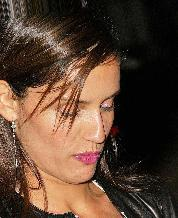
\includegraphics[width=.4\linewidth]{input-img-for-mask.jpg}
                  \caption{Bemeneti kép}
                \end{subfigure}%
                \begin{subfigure}{.5\textwidth}
                  \centering
                  
\includegraphics[width=.4\linewidth]{generated-mask.png}
                  \caption{Alapigazság maszk}
                \end{subfigure}
                \caption{Példa a szegmentáló hálózat tanítási adataira.}
                \label{fig:trainset-mask}
            \end{figure}

             A(z) \ref{fig:trainset-mask}. ábra egy példát ábrázol egy bemeneti képpel (bal oldal) és a hozzá tartozó, tanításhoz elkészített alapigazság maszkkal (jobb oldal).

            \subsubsection{Képek előfeldolgozása}

            Mielőtt a bemeneti képeket átadnánk az arcrekonstrukciós modellünknek, a képek előfeldolgozására van szükség. Az előfeldolgozás a képek átméretezését, és az arc körülvágását foglalja magában.

            A kép egy adott méretre történő átméretezésére gyakran van szükség, amikor olyan mély tanulási modellekkel dolgozunk, amelyeknek rögzített bemeneti mérete van. A kép átméretezésével biztosíthatjuk, hogy a képnek ugyanazok a méretei legyenek, mint az arcrekonstrukciós hálózat bemeneti rétegének. Ez segíthet elkerülni az esetleges torzulásokat amelyek akkor keletkezhetnek, ha egy eltérő méretű képet táplálunk a hálózatba.

            A vágás viszont a kép egy adott részének kiválasztását jelenti, amelyet a hálózat bemenetként használ. Az arc rekonstrukciója esetén ez segíthet eltávolítani a háttérben lévő vagy irreleváns információkat a képről, lehetővé téve a hálózat számára, hogy kizárólag az arcvonásokra koncentráljon. A képkivágás emellett segíthet az arc képen belüli tájolásának és pozíciójának egységesítésében is, ami megkönnyítheti a hálózat számára a szükséges jellemzők kinyerését és az arc pontos rekonstruálását.

            A képeknek az arcrekonstrukciós hálózatba való bevitele előtti átméretezésével és vágásával biztosíthatjuk, hogy a hálózat csak a releváns arcvonásokat kapja meg, egységes orientációval és mérettel, ami végső soron javíthatja a rekonstrukció pontosságát.
            
            \subsubsection{Hálózat felépítése}

            \begin{figure}[h!]	
        		\centering
        		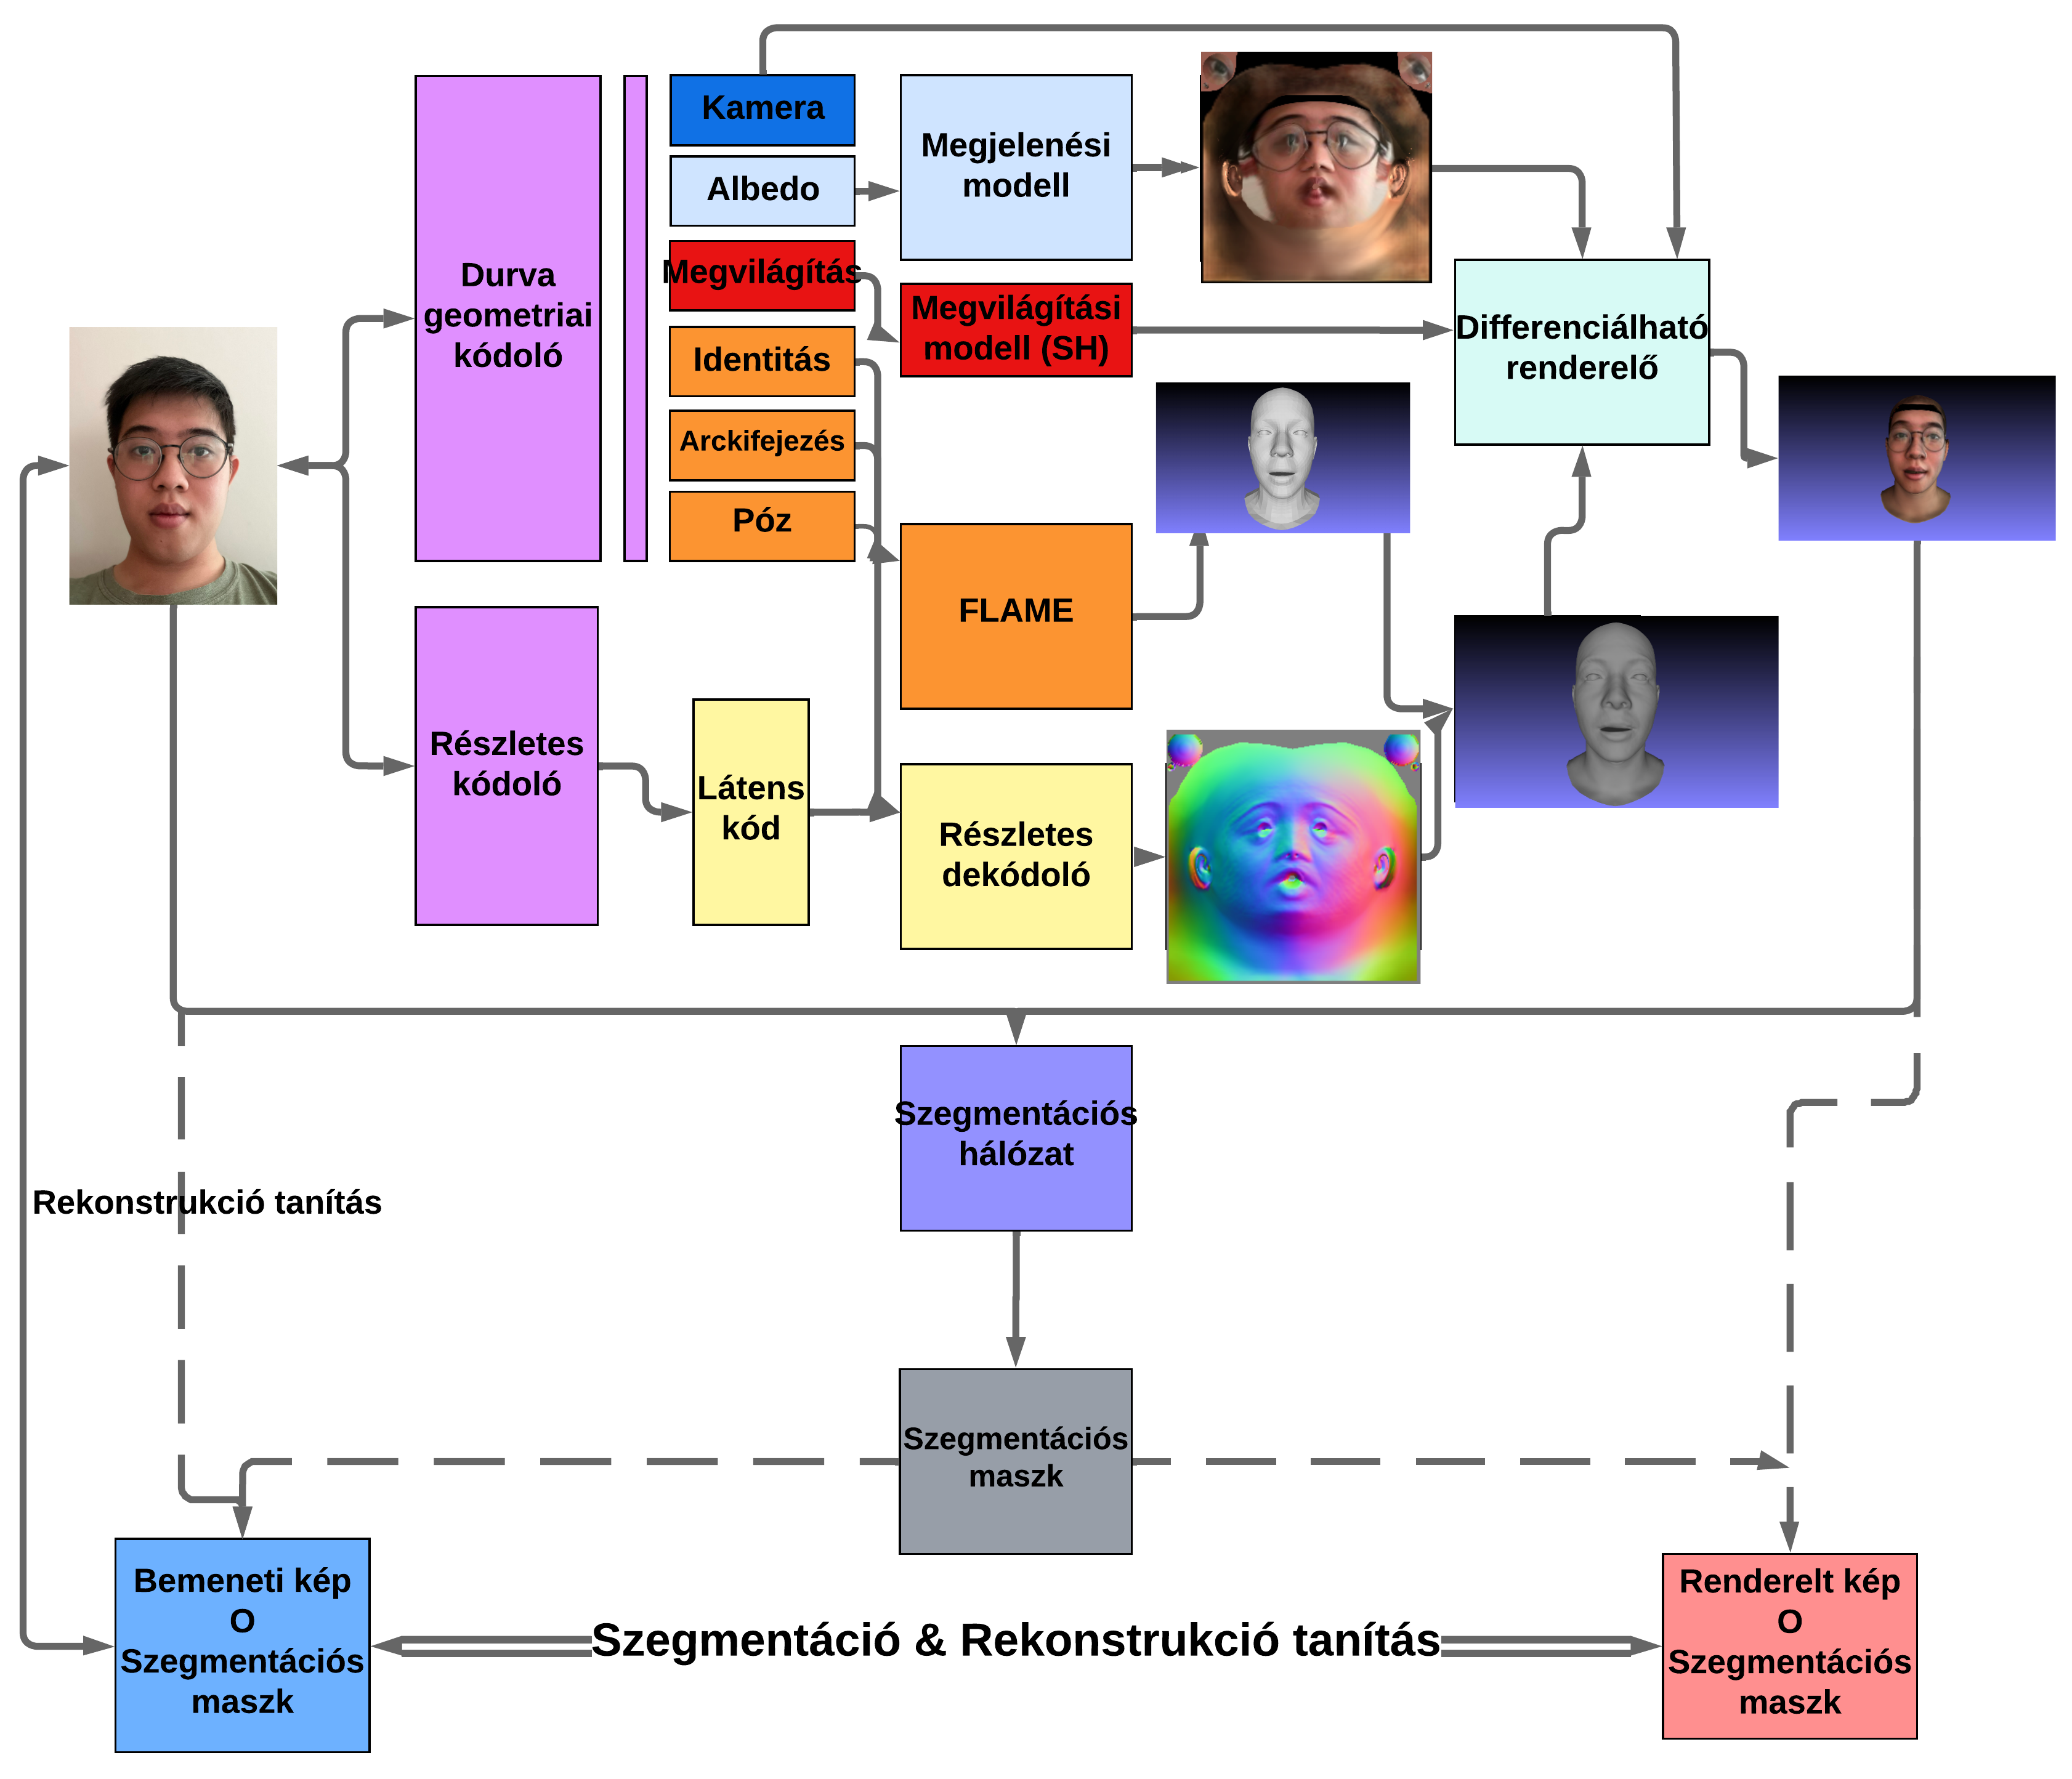
\includegraphics[width=1\linewidth]{pipelinehun}
        		\caption{  A rekonstrukciós hálózat tanítási futószalagja.}
                \label{fig:pipeline}
        	\end{figure}

            
        	Az arcreskonstrukciós modellünket a(z) \ref{fig:pipeline}. ábrán szemléltetjük. A hálózatot PyTorch
        	keretrendszerben fejlesztettük.
        	A DECA módszerét követve a hálózatunk első lépése egy
        	ResNet-50 modulból és egy teljesen összekapcsolt rétegből álló kódoló
        	$E_{c}$, amely egy 2D-s kontrollálatlan környezetben készült képet kap bementként, majd visszaadja annak alacsony dimenzós látens kódját.
         
            A látens kód a $FLAME$
        	paramétereket (durva geometriát) $\beta$ $\psi$ $\theta$, valamint az albedo együtthatókat
        	$\alpha$, kamera $c$, és megvilágítási $l$ paramétereket tartalmazza.
        	Az albedó paramétereket megkapja
        	bemenetként a megjelenési modell, amely a Basel Face Model (BFM)
        	lineáris albedó alterét alakítja át a $FLAME$ UV elrendezésébe,
        	hogy kompatibilissé tegye azt $FLAME$-el A megvilágítási paramétereket
        	a megvilágítási modell kapja meg bemenetként, amely
        	a gömbharmónia (Spherical Harmonics/SH) alapú.
         
            A durva geometria
        	paramétereit felhasználva a $FLAME$ modell egy durva alakzatot készít az
        	arcról. 
 
            A DECA által javasolt részletes dekódolóba a 128 db személyspecifikus jellemzőt betáplálva egy UV eltolódási térképet készítünk. A durva alakot és az eltolódási térképet felhasználva egy részletes alakzatot készítünk, amelyet átadva a megvilágítási modellel,
        	az albedó térképpel, és a kamera paraméterekkel a differenciálható renderelőnek egy részletes rekonstruált textúrázott 3D-s fejet kapunk kimenetül.

 
        	A $FOCUS$ megközelítéséhez hasonlóan a szegmentáló hálózatunk átveszi
        	a bemeneti képet és a hozzá tartozó részletes rekonstruált 3D-s fejet, majd
        	megjósolja a bináris maszkot.

         \subsubsection{Fontosabb komponensek megvalósítása}

         \paragraph{Megjelenési modell}

        A FLAME nem rendelkezik megjelenési modellel, ezért Yao és tsai. \cite{deca} ajánlására a BFM lineáris albedó altérét alakítjuk át
        a FLAME UV elrendezésébe, hogy kompatibilis legyen a FLAME-mel. A megjelenési modell egy UV albedótérképet ($A(\alpha) \in \mathbb{R}^{d \times d \times 3}$) ad vissza, ahol $\alpha \in \mathbb{R}^{|\alpha|}$ az albedó paramétereket jelöli.  
         
         \paragraph{Kamera modell}

          A meglévő arcadatbázisokban szereplő képek gyakran távolról készültek.
          Ezért a DECA ortográfiai kameramodelljét használjuk a 3D háló képi térbe történő kivetítéséhez.
          Az arc csúcsait a képre vetítjük, mint $v = s\Pi(M_{i}) + t$, ahol
          $M_{i} \in \mathbb{R}^{3}$ az $M$ egy csúcsa, $\Pi \in \mathbb{R}^{2 \times 3}$ az ortográfiai 3D-2D vetítési mátrix, $s \in \mathbb{R}$ és $t \in \mathbb{R}^{2}$ pedig az izotróp méretarányt és a 2D eltolást jelölik. Az $s$ és $t$ paramétereket összefoglalóan $c$-vel jelöljük.
                     
         \paragraph{Kódoló}

            Mint említettük, a DECA kódoló hálózatát használjuk fel a személyspecifikus látens kód kinyerésére a bemeneti képekből.
            
            Az encoders.py modulban található ResnetEncoder osztály az arcrekonstrukciós modellben használt $E_c$ és $E_d$ kódoló  hálózatok PyTorch implementációja, amely a személyspecifikus jellemzők, valamint a FLAME paraméterek kinyerésére szolgál. 
            A kódoló bemenetként egy arc képét veszi, és egy látens kódot állít elő, amelyet a dekódoló/generátorhálózat bemeneteként használ.
            
            A ResnetEncoder osztály a PyTorch nn.Module osztály alosztálya, és konvolúciós rétegek és reziduális blokkok sorozatából áll.
            A kódoló bemenete egy RGB arckép, amely egy sor konvolúciós rétegen halad át az alacsony szintű jellemzők kinyerése érdekében.
            Ezek az alacsony szintű jellemzők ezután egy sor maradék blokkon haladnak keresztül, amelyek a magasabb szintű jellemzők rögzítésére és a jellemzőtérkép dimenziójának csökkentésére szolgálnak.
            
            A ResnetEncoder osztály a ResNet architektúra módosított változatát használja, amely egy képfelismerési feladatokban általánosan használt mély neurális hálózati architektúra.
            A ResnetEncoder osztályban használt módosított ResNet architektúra több konvolúciós réteget tartalmaz, amelyet több szakaszba csoportosított maradék blokkok sora követ.
            Minden egyes szakasz olyan maradék blokkokat tartalmaz, amelyek fokozatosan csökkentik a jellemzőtérkép méretét és növelik a jellemzőcsatornák számát.
            
            A ResnetEncoder osztály több lemintavételezési réteget is tartalmaz, amelyek a jellemzőtérkép méretének csökkentésére és a modell receptív mezejének növelésére szolgálnak.
            A lemintavételező rétegek a konvolúciós rétegek és a max-pooling rétegek kombinációját használják a jellemzőtérkép méretének 2-szeresére való csökkentésére.
            
            A ResnetEncoder osztály kimenete egy lapított jellemzővektor, amely több teljesen összekapcsolt rétegen halad át a látens kód előállításához. 
            A teljesen összekapcsolt rétegek közé tartoznak a kieső rétegek, amelyek a túlillesztés megelőzésére és a modell általánosítási teljesítményének javítására szolgálnak.
            
            A ResnetEncoder osztály az ellentétes veszteség, a rekonstrukciós veszteség és a regularizációs veszteség kombinációjával tanítható.
            Az ellentétes veszteséget arra használjuk, hogy a látens kódot arra ösztönözzük, hogy ne lehessen megkülönböztetni a valódi látens kódoktól, 
            míg a rekonstrukciós veszteség a generált 3D háló és az alapigazság 3D háló közötti különbség minimalizálására szolgál.
            A regularizációs veszteséget a túlillesztés megakadályozására és a modell sima és reális látens kódok tanulására ösztönzi.
            
            Összességében az encoders.py modulban található ResnetEncoder osztály egy hatékony eszköz az arcképek látens kódokká történő kódolásához, amelyek a dekódoló-/generátorhálózat bemeneteként használhatók. 
            Az osztály az arcrekonstrukciós modellben használt kódolóhálózatok hasznos implementációját biztosítja, és könnyen adaptálható más képalapú 3D rekonstrukciós feladatokhoz.
         
         \paragraph{Dekódoló}

             A decoders.py modulban található Generator osztály a DECA modellben használt dekódoló PyTorch implementációja, amely egyetlen képből történő 3D arc rekonstrukciójára szolgál.
             A generátor bemenetként egy látens kódot és egy kifejezési együtthatókból álló készletet fogad el, és létrehozza a rekonstruált arc 3D hálóját.
             
             A Generator osztály a PyTorch nn.Module osztály alosztálya, és több rétegből áll, beleértve a teljesen összekapcsolt rétegeket, a konvolúciós rétegeket és a maradék blokkokat. 
             A generátor bemenete a látens kód és a kifejezési együtthatók összevonása, amelyek több teljesen összekapcsolt rétegen keresztülhaladva egy jellemzővektort generálnak. 
             Ezt a jellemzővektort ezután átformáljuk, és egy sor konvolúciós rétegen keresztül vezetjük át a végső 3D háló előállításához.
            
             A generátor osztály több maradék blokkot is tartalmaz, amelyek a modell pontosságának és stabilitásának javítására szolgálnak. 
             A maradék blokkok konvolúciós rétegek sorozatából és egy kihagyásos kapcsolatból állnak, amely a bemenetet hozzáadja a konvolúciós rétegek kimenetéhez.
             Ez lehetővé teszi, hogy a modell megtanulja a maradék jellemzőket, amelyeket a végső kimenet finomítására használ.
             
             A Generator osztály több kötegnormalizációs réteget is tartalmaz, amelyek a konvolúciós rétegek kimenetének normalizálására szolgálnak.
             Az példány normalizálás segít javítani a modell stabilitását és konvergenciáját, és különösen hasznos a képszintézist tartalmazó generatív modellek esetében.
             
             A Generator osztály tanítható az ellentétes veszteség, a rekonstrukciós veszteség és a regularizációs veszteség kombinációjával.
             Az ellentétes veszteség arra ösztönzi a generált 3D hálót, hogy megkülönböztethetetlen legyen a valós 3D hálótól, míg a rekonstrukciós veszteség a generált 3D háló és az alapigazság 3D háló közötti különbség minimalizálására szolgál. 
             A regularizációs veszteséget a túlillesztés megakadályozására és a modell sima és valósághű 3D-hálók megtanulására ösztönzi.
             
             Összességében a decoders.py moduljában található Generator osztály egy hatékony eszköz a 3D arcok hálóinak egyetlen képből történő generálásához,
             valamint a modellben használt generátorhálózat hasznos implementációját biztosítja.
                     
         \paragraph{ResNet architektúra}

            Az arcrekonstrukciós hálózat az frnet.py modulban a DECA \cite{deca} által implementált ResNet architektúrát használja a bemeneti képek jellemzőinek kinyerésére. 
            A ResNet architektúra több építőblokkból áll, köztük a BasicBlock, a Bottleneck és a ResNet elemekből.
            
            A BasicBlock osztály a PyTorch nn.Module osztály alosztálya, és két konvolúciós rétegből áll, amelyet egy kötegelt normalizáló réteg és egy ReLU aktivációs függvény követ.
            A bemenet az első konvolúciós rétegen, majd a kötegelt normalizáló és a ReLU rétegen, végül pedig a második konvolúciós rétegen halad át. 
            A második konvolúciós réteg kimenete hozzáadódik a bemenethez a maradék kapcsolat létrehozásához.
            
            A Bottleneck osztály hasonló a BasicBlockhoz, de kettő helyett három konvolúciós réteget tartalmaz.
            Az első konvolúciós réteg csökkenti a bemeneti csatornák számát, a második konvolúciós réteg 3x3-as konvolúciót alkalmaz, a harmadik konvolúciós réteg pedig növeli a kimeneti csatornák számát.
            A BasicBlockhoz hasonlóan a Bottleneck is tartalmaz kötegnormalizálást és ReLU aktiválási függvényt, és egy maradékkapcsolatot használ az utolsó konvolúciós réteg kimenetének a bemenethez való hozzáadásához.
            
            A ResNet osztály a PyTorch nn.Module osztály alosztálya, és egy sor egymásra helyezett BasicBlock vagy Bottleneck rétegből áll.
            A ResNet osztály több lemintavételező réteget tartalmaz, amelyek a jellemzőtérkép méretét felére csökkentik, és több felmintavételező réteget, amelyek a jellemzőtérkép méretét növelik.
            A ResNet osztály képosztályozásra és jellemzőkinyerésre egyaránt használható.
             
            Tehát a ResNet architektúrát használjuk az arcképek jellemzőinek kinyerésére. A bemeneti kép először több konvolúciós rétegen halad át az alacsony szintű jellemzők kinyerése érdekében.
            Ezek az alacsony szintű jellemzők ezután több BasicBlock vagy Bottleneck rétegen haladnak át a magasabb szintű jellemzők rögzítése érdekében. 
            Az utolsó ResNet réteg kimenete egy jellemzőtérkép, amelyet több felszűrő réteg bemeneteként használnak, amelyek az arcrégiós maszkok végső készletét állítják elő.
            
            Összességében a frnet.py modulban található BasicBlock, Bottleneck és ResNet osztályok a ResNet architektúra hatékony megvalósítását biztosítják, 
            amely a képfeldolgozási feladatok széles skálájához használható, beleértve az arc régióinak szegmentálását és a 3D arc rekonstrukcióját. \\

            A ResNet implementációját a kódoló hálózatokban használjuk fel és módosítjuk azt a személyspecifikus jellemzők és a FLAME paraméterek kinyerése érdekében
                     
         \paragraph{Sztenderd raszterizáló}
             A sztenderd raszterizáló a rasterizer.py fájlban van implementálva.
             Ez a raszterizáló egy 3D-s archálót kap, amelyet csúcsok és lapok halmaza reprezentál, és egy 2D-s képsíkra vetíti, hogy az arc textúrázott képét létrehozza.
             A DECA \cite{deca} által implementált raszterizáló a következő lépések szerint működik:
             \begin{enumerate}
                 \item \textbf{Perspektív vetítési mátrix létrehozása}:
                        A perspektív vetítési mátrix egy 4x4-es mátrix, amely a 3D koordinátákat 2D képkoordinátákra képezi le. 
            	        A mátrix kiszámítása a kamera kalibrációs paramétereinek felhasználásával történik, amelyek közé tartozik a kamera belső mátrixa, külső mátrixa és a képméret. 
                        Az belső mátrix a kamera belső paramétereit, például a fókusztávolságot, a főpontot, 
                        és a dőlést tartalmazza, míg az külső mátrix a kamera helyzetét és tájolását a világkoordináta-rendszerben.
                 
                 \item \textbf{A vetítési mátrix alkalmazása a a csúcsokra}:
         
                        A 3D archáló csúcsait homogén koordinátákká alakítjuk át egy negyedik dimenzió hozzáadásával, amelynek értéke 1. 
                    	Ezután a perspektivikus vetítési mátrixot alkalmazzuk a csúcsokra, hogy megkapjuk a megfelelő 2D-s képkoordinátákat. 
                    	A 2D képkoordinátákat úgy kapjuk meg, hogy az x és y koordinátákat elosztjuk a homogén w koordinátával.
     
                 \item \textbf{A háromszögek határoló dobozainak kiszámítása}:
         
                        A háromszögek határoló dobozait az archálóban 2D-s képkoordinátákban kell kiszámítani.
                    	A határoló dobozokat a háromszög csúcsainak minimális és maximális x és y koordinátái határozzák meg.
     
                 \item \textbf{A háromszögek raszterizálása}:
         
                        A raszterizáló az archáló minden egyes háromszögéhez kiszámít egy maszkot, amely jelzi, hogy a 2D-s kép mely pixelei tartoznak a háromszöghöz. 
                        A maszk kiszámítása a háromszög csúcsainak baricentrikus koordinátáinak interpolációjával történik a háromszög határoló dobozán.
                    	A baricentrikus koordinátákat a csúcsok súlyaként határozzuk meg, amelyek összege egy, és a háromszög textúrakoordinátáinak és csúcsnormálisainak interpolálásához használjuk.
     
                \item \textbf{Textúra leképezése}:
         
                        A raszterizáló a raszterizált háromszögekhez a textúra hozzárendelésével  hozza létre a végső képet. 
                        A textúratérképezés során a háromszögben lévő minden egyes pixel textúrakoordinátáit a baricentrikus koordináták és a háromszög csúcsainak textúrakoordinátái alapján számítja ki.
            	        Ezután a textúrakoordinátákat a megfelelő helyen a textúrakép mintavételezéséhez használjuk, és a mintavételezett texel színértékét rendeljük a pixelhez.
     
                 \item \textbf{Alfa keverés}:
                 
                        A raszterizáló az átlátszóság kezelése érdekében alfa keverést alkalmaz a raszterizált háromszögekre. 
                    	A háromszögben lévő egyes pixelek alfa-értékét a baricentrikus koordináták és a háromszög csúcsainak alfa-értékei alapján számítja ki. 
                    	Ezután az alfa-értékek segítségével a pixel színértéke a háttérszínnel keveredik.
     
            \end{enumerate}
     
             Összességében a sztenderd raszterizáló a 3D archáló renderelésének robusztus és hatékony megvalósítását biztosítja.
             A raszterizáló testreszabható és bővíthető, hogy különböző textúra leképezési és keverési technikákat, valamint különböző renderelési lehetőségeket, például világítást és árnyékolást alkalmazzon.
         
        \paragraph{Differenciálható renderelő}
             A differenciálható renderelés egy olyan renderelési módszer, amely a kamera paraméterei, a csúcsok pozíciói és a textúra leképezések alapján egy 3D-s arc háló 2D-s képét generálja. A metódus DECA \cite{deca} által készített és általunk felhasznált implementációját a renderer.py SRenderY osztálya tartalmazza. 

             Az SRenderY módszer mükődése:
            
             \begin{enumerate}
             
                \item Egy üres (H, W, 3) méretű képpuffer inicializálása, ahol H és W a kimeneti kép magassága és szélessége pixelben, 3 pedig a színcsatornák száma (piros, zöld és kék).
            
                \item A 3D archáló minden egyes háromszögéhez kiszámítja a 2D-s vetületét a képsíkra a kamera paraméterei alapján. Ez a perspektivikus vetítési egyenlet segítségével történik, 
                amely a világkoordinátarendszer 3D pontjait a képsík 2D pontjaivá alakítja át.
            
                \item A kivetített háromszög határoló dobozán belüli minden egyes pixel esetében ellenőrzésre kerül a baricentrikus koordináta módszerrel, hogy a pixel a háromszögben van-e. 
                Ennek során kiszámítja a pixel baricentrikus koordinátáit a háromszög csúcsaihoz képest, és ellenőrizzük, hogy ezek mindegyike pozitív-e.
             
                \item Ha a képpont a háromszög belsejében van, akkor az inverz perspektivikus vetítési egyenlet segítségével kiszámítja a megfelelő 3D pozícióját az arc hálóján.
            
                \item A pixel textúrakoordinátáinak interpolálása a háromszög csúcsainak textúrakoordinátáiból a baricentrikus koordináták segítségével.
            
                \item Az interpolált textúrakoordináták felhasználása a megfelelő helyen lévő textúratérkép színértékének mintavételezéséhez.
            
                \item A színérték megszorzása a megvilágítási értékkel, amelyet a pixel felszíni normálisa és a fény iránya közötti skalárszorzataként számítunk ki.
            
                \item A színérték felhalmozása a képponthoz a képpufferben.
            
                \item A 2-8. lépés megismétlése a 3D archáló összes háromszögére.
            
                \item Visszaadja a végső képpuffer képét kimenetként.
                
             \end{enumerate}
            
            Összességében az SRenderY módszer egy sztenderd raszterizáció-alapú renderelési algoritmus, amely figyelembe veszi a perspektivikus vetítést,
            textúratérképezést és a megvilágítást. A DECA keretrendszerre építve 3D-s archáló 2D-s képének létrehozására használjuk.

        \paragraph{Megvilágítás hozzáadása}
            A renderer.py add\_SHlight metódusa egy olyan módszer, amely gömbharmonikus (SH) megvilágítást ad hozzá egy 3D-s archáló 2D-s képéhez.

            Az add\_SHlight (\textit{Spherical Harmonics}) módszer működése a DECA \cite{deca} általi implementáció alapján:
            
            \begin{enumerate}
                \item Egy üres (H, W, 3) méretű képpuffer inicializálása, ahol H és W a bemeneti kép magassága és szélessége pixelben, 3 pedig a színcsatornák száma (piros, zöld és kék).
            
                \item Kiszámítja a világítás gömbharmonikus (SH) együtthatóit az SH-projekciós módszerrel, amely a világítási függvény ortonormális SH-alapfüggvények halmazára való vetítését jelenti.
            
                \item A bemeneti kép minden egyes pixelére kiszámolja az archáló megfelelő 3D pontjának felületi normálisát. Ez elvégezhető az arc geometriájának a 2D képkoordinátákhoz viszonyított részleges deriváltjainak segítségével.
            
                \item Értékelje ki az SH megvilágítási függvényt a képpont felületi normálisán a 2. lépés SH együtthatóinak felhasználásával. Ehhez ki kell számítani az SH alapfüggvények és a felületi normális vektor közötti skalárszorzatot.
            
                \item Megszorozza a bemeneti kép pixelének színértékét a 4. lépésben kiszámított SH megvilágítási értékkel.
            
                \item A kapott színértéket a [0, 255] tartományba kell szorítani, hogy a 8 bites színértékek érvényes tartományába essen.
            
                \item A kimeneti képpuffer kép pixelének színét a rögzített színértékre állítja.
            
                \item Megismétli a 3-7. lépést a bemeneti kép összes pixelére.
            
                \item Visszaadja a végső képpuffer képét kimenetként.
            
                
            \end{enumerate}
            
            Összességében az add\_SHlight módszer egy meglehetősen szabványos módszer SH megvilágítás hozzáadására egy 3D-s arc háló 2D-s képéhez. A világítási függvény SH-együtthatóinak kiszámítását, 
            az SH-világítás kiértékelését minden egyes felületi normálisnál, és az egyes pixelek színértékének megszorzását az így kapott világítási értékkel foglalja magában. 
            Ezt a módszert a DECA keretrendszer alapján a 3D-s arcok SH megvilágítással ellátott hálóinak valósághű 2D-s képeinek létrehozására használjuk.

        \paragraph{Normáltérkép kiszámítása eltolódási térképből}

            A DECA \cite{deca} által implementált displacement2normal függvény arra szolgál, hogy az elmozdulási térképből kiszámítsa a normáltérképet, amelyre a renderelésnél lesz szükségünk. 
            A számítógépes grafikában az elmozdulási térkép egy olyan textúra, amely egy objektum felületének elmozdulását kódolja.
            A textúrában lévő elmozdulási értékek jellemzően a felületre merőleges irányban vannak meghatározva, ami azt jelenti, hogy felhasználhatóak a normáltérkép kiszámításához.
            
            A displacement2normal függvény bemenetként egy elmozdulási térképet és a térképen lévő pixelek textúrakoordinátáit veszi fel. 
            Az elmozdulási térképet szürkeárnyalatos képnek tekintjük, ahol az értékek a felületre merőleges irányú elmozdulást jelölik.
            A textúrakoordináták a textúra képpontjainak 2D koordinátái.
            
            A normáltérkép kiszámításához a függvény először kiszámítja az elmozdulási térkép részleges deriváltjait a textúrakoordinátákhoz képest.
            Ezek a parciális deriváltak a felület x és y irányú meredekségét jelentik. A parciális deriváltakat ezután a felület normális vektorának kiszámítására használjuk minden egyes pixelnél.
            
            A normálvektor kiszámításához a függvény először kiszámítja a felület érintővektorát és bitangens vektorát.
            Az érintővektort az x irányú parciális derivált és az (1, 0, 0) vektor keresztszorzataként számoljuk ki. 
            A bitangens vektor az y irányú parciális derivált és a (0, 1, 0) vektor keresztszorzataként számítandó. 
            Végül a normálvektort az érintővektor és a bitangens vektor keresztszorzataként számítjuk ki.
            
            Az így kapott normáltérkép egy 3 csatornás kép, ahol minden egyes pixel egy normálvektort képvisel. 
            A normálvektor x, y és z komponenseit a vörös, zöld és kék csatornákban kódoljuk. 
            A normálvektort úgy normalizáljuk, hogy egységnyi hosszúságú legyen.
            
            Összességében a displacement2normal függvény lehetővé teszi az elmozdulás-térkép normál-térképpé alakítását, amely egy objektum felületének nagy felbontású részletekkel történő szimulálására használható.

    \subsubsection{Veszteségfüggvények}
        \paragraph{Arcrekonstrukciós hálózat veszteségfüggvényei} \label{coarselosssection}

            Az arcrekonstrukciós hálózat a tanítás során a következő veszteségfüggvényt minimalizálja:

            \begin{equation} \label{coarseloss}
                L   =  &\lambda_{lmk}L_{lmk}   &+  &\lambda_{eye}L_{eye}   &+  &\lambda_{pho}L_{pho}   &+  &\lambda_{id}L_{id} &+  &L_{reg}  
            \end{equation}
            ,ahol $\lambda \in \mathbb{R}$ az egyes költségfüggvényekhez tartozó súlyértékeket, 
            $L_{lmk}$ az arcpont reprojekciós veszteséget, 
            $L_{eye}$ a szemzárási veszteséget,
            $L_{pho}$ a fotometriai veszteséget,
            $L_{id}$ az identitás veszteséget és 
            $L_{reg}$ a regularizációt jelöli.

            Tehát az arcrekonstrukciós hálózat veszteségfüggvénye hat különböző veszteségfüggvény lineáris kombinációjából tevődik össze. A hat veszteségfüggvény:

            \begin{enumerate}
                \item Az \textit{arcpont reprojekciós veszteség} ($L_{lmk}$) méri a
                az alapigazság szerinti 2D-s arc $k_{i}$ tájékozódási pontjai és az azoknak megfelelő
                a FLAME modell felszínén található  $M_{i} \in \mathbb{R}^3$ tájékozódási pontok között, amelyeket a becsült kameramodell vetít a képre. Az
                arcpont reprojekciós veszteséget a következőképpen határozzuk meg:

                \begin{equation}
                    &L_{lmk} &= \sum_{i=1}^{68} || k_{i} - s\Pi(M_{i}) + t ||_{1}
                \end{equation}
                
                \item A \textit{szemzárási veszteség} kiszámítja a felső és alsó szemhéjon lévő $k_{i}$ és $k_{j}$ tájékozódási pontok relatív eltolódását, és méri a FLAME felszínén lévő $M_{i}$ és $M_{j}$ megfelelő tájékozódási pontok képre vetített eltolódásának különbségét. Formálisan a veszteség a következő:

                \begin{equation}
                    L_{eye} = \sum_{(i,j) \in E} || k_{i} - k_{j} - s\Pi(M_{i} - M_{j}) ||_{1}
                \end{equation}
                , ahol $E$ a felső/alsó szemhéj tájékozódási pontpárok halmaza.  
              $L_{eye}$ a szemhéjak tájékozódási pontjai közötti relatív különbséget bünteti. 
              Mivel a szemzárási veszteség transzlációs invariáns, 
              kevésbé érzékeny a vetített 3D-s arc és a kép közötti eltérésre az $L_{lmk}$-hoz képest. 
                
                \item A \textit{fotometriai veszteség} az $I$ bemeneti kép és az $I_{r}$ rekonstruált kép közötti hibát a következőképpen számítja ki:

                \begin{equation}
                    L_{pho} = || V_{1}\bigodot(I -I_{r}) ||_{1,1}
                \end{equation}
                , ahol $V_{1}$ az arcmaszk, amely értéke 1 az arcbőr tartományában és 0 máshol, és $\bigodot$ a Hadamard-szorzatot jelöli.
                A hiba csak az arc régiójában történő kiszámítása robusztusságot biztosít a gyakori elfedésekkel szemben, mint a haj, ruha, napszemüveg. Enélkül a megjósolt albedó a takarás színét is figyelembe veszi, ami távol állhat a bőrszíntől, ami természetellenes megjelenítést eredményez.
                
                \item Az \textit{identitás veszteség} felhasználásának hatékonyságát a valósághűbb arcformák előállítása érdekében a FOCUS és a DECA is bizonyította. Ennek hatására mi is Cao és tsai. \cite{pretrained-resnet} előzetesen betanított arcfelismerő hálózatát használjuk, hogy a tanítás során identitásvesztést alkalmazzunk.
                
                Az arcfelismerő hálózat $f$ a renderelt kép $I_{r}$ és a bemeneti kép $I$ jellemző beágyazásait adja vissza, majd az identitásveszteség a két beágyazás közötti koszinusz hasonlóságot határozza meg.

                Az identitás veszteséget a következőképpen számítjuk ki:

                \begin{equation}
                    L_{id} = 1 - \frac{f(I)f(I_{r})}{|| f(I) ||_{2} \cdot || f(I_{r}) ||_{2}}
                \end{equation}
                A beágyazások közötti hiba kiszámításával a veszteségfüggvény arra ösztönzi
                a renderelt képet, hogy megragadja a személy alapvető tulajdonságait.
                Biztosítja, hogy a megjelenített kép hasonlítson a bemeneti alanyra.
                
                \item $L_{reg}$ az alakot $E_{\beta} = ||\beta||_{2}^{2}$, az arckifejezést $E_{\psi} = ||\psi||_{2}^{2}$, és az albedót $E_{\alpha} = ||\alpha||_{2}^{2}$ regularizálja. $L_{reg}$ a következőképpen számítható ki:

                \begin{equation}
                    L_{reg} = \lambda_{E_{\beta}}E_{\beta} + \lambda_{E_{\psi}}E_{\psi} + \lambda_{E_{\alpha}}E_{\alpha} 
                \end{equation}
                , ahol $\lambda$ jelöli az egyes regularizációkhoz tartozó súlyértékeket.
                
            \end{enumerate}

            Az egyes költségfüggvények a DECA által definiált költségfüggvények közül kerültek kiválasztásra.
        
        \paragraph{Szegmentáló hálózat veszteségfüggvényei} \label{unetseg}

            Projektünk célja egy robusztus 3D arcrekonstrukciós rendszer létrehozása, amely egy gyengén felügyelt tanulási technikákkal tanított szegmentáló hálózatot használ. Ennek eléréséhez a Yu Deng és tsai. \cite{focus} tanulmányából merítünk ihletet. 

            Célkitűzésünk, hogy hasonló szegmentáló hálózatot és veszteségfüggvényeket valósítsunk meg a 3D-s arc rekonstrukciójához a rendszer pontosságának és robusztusságának javítására összpontosítva. A Yu Deng és tsai. \cite{focus} által javasolt, gyengén felügyelt tanulási technikák és veszteségfüggvények felhasználásával reméljük, hogy lenyűgöző eredményeket érhetünk el a 3D arcrekonstrukciós rendszerünkben.

            A javasolt veszteségek a következők:

            \begin{equation}
                \label{nbr}
                L_{nbr} = \sum_{x \in \Omega}\Big|\Big|\min_{\forall x^{'} \in N(x)}||I_{T}(x)-I_(R)(x_{'})||\Big|\Big|_{2}^{2}
            \end{equation}

            A(z) \ref{nbr}. egyenletben szereplő pixel-szintű szomszédos veszteség, $L_{nbr}$ , összehasonlítja a célkép $x$ helyén lévő $I_{T}(x)$ pixeleit a renderelt képen a szomszédos régióban lévő $N(x)$ pixelekkel. 

            Megjegyzendő, hogy ez csak az arcon belüli régiót figyeli, $\omega$-t, amelyet a szegmentáló hálózat előre jelez. Egy nagyobb szomszédos veszteség $x$-nél azt jelzi, hogy ez a képpont nem illeszkedik jól és valószínűbb, hogy kiugró érték.
                

            \begin{equation}\label{dist}
                L_{dist} = \cos(F(I_{T} \bigodot M),(I_{R} \bigodot M))  
            \end{equation}

            Hasonlóképpen, a \ref{dist}. egyenletben szereplő $L_{dist}$ a bemeneti és a rekonstruált arc perceptuális szintű összehasonlítására szolgál.

            A(z) \ref{nbr} és \ref{dist} egyenletek célja a maszk zsugorítása a kiugró értékeken, ahol a pixel-szintű és az perceptuális különbségek nagyok.

            Minden egyéb megkötés nélkül a szegmentáló hálózat egy teljesen nulla maszkot adna ki, hogy mindkettő 0 legyen. Ha van egy kényszer, amely arra ösztönzi a hálózatot, hogy megőrizze a bizonyos képrészeket, akkor a kisebb veszteséggel rendelkező részek nagyobb valószínűséggel megmaradnak.

            Ezért a következő egyenleteket használjuk a fenti két veszteségfüggvény ellensúlyozására.
                
            \begin{equation} \label{area}
                L_{area} = -S_{M}/S_{R}
            \end{equation}

            A(z) \ref{area}. egyenlet célja hogy megnövelje a becsült arcpixelek száma, $S_{M}$, és a renderelt arctérségben lévő pixelek száma,$S_{R}$ közötti arányt. Ez megakadályozza hogy a szegmentáló hálózatot attól, hogy túl sok pixelt vessen el.
                
            \begin{equation} \label{presv}
                L_{presv} = \cos(F(I_{T} \bigodot M),F(I_{R}))
            \end{equation}

            A(z) \ref{presv}. egyenlet, biztosítja, hogy a perceptuális
            arcjellemzők hasonlóak maradjanak, miután a kiugró értékek a bemeneti képen ki lettek maszkolva és arra ösztönzi a modellt, hogy megőrizze a látható arcterület minél nagyobb részét.

            \begin{equation} \label{bin}
                L_{bin} = -\sum\limits_{x}(M(x) - 0.5)^2
            \end{equation}

            Használunk egy további regularizációs egyenletet (\ref{bin}), $L_{bin}$-t, hogy az armaszk $M$ bináris legyen.

            A szegmentáló hálózat tanításának teljes vesztesége a következő:

            \begin{equation}
                L_{S} = \eta{1}L_{nbr} + \eta{2}L_{dist} + \eta{3}L_{area} + \eta{4}L_{presv} + \eta{5}L_{bin}
            \end{equation}

            ahol, $\eta{1} = 15 \quad \eta{2} = 3 \quad \eta{3} = 0.5 \quad \eta{4} = 0.25 \quad \eta{5} = 10$.
            
    \subsubsection{Tanítás}
        Egy mély tanulási modell betanítása magában foglalja a modell paramétereinek iteratív beállítását, hogy minimalizáljon egy kiválasztott veszteségfüggvényt egy adott adathalmazon. A cél a modell optimalizálása, hogy pontos előrejelzéseket adjon az új, még nem látott adatokra. Az előtanítást gyakran használják a modell tanításának első lépéseként, különösen olyan esetekben, amikor a célfeladat egy korábban megtanult feladathoz kapcsolódik.

        Az előtanítás során a modellt egy kapcsolódó feladatra tanítják be egy nagy adathalmazon, jellemzően felügyelet nélkül, hogy megtanulják a bemeneti adatok általános jellemzőit. Ezután a modellt a célfeladaton finomhangolják egy kisebb, jellemzően felügyelt adathalmaz segítségével, hogy javítsák a teljesítményét a célfeladaton. Az előtanítás javíthatja a modell teljesítményét azáltal, hogy jó inicializálást biztosít a modell paraméterei számára, átadja a kapcsolódó feladatból származó tudást a célfeladatra, és javítja a modell korlátozott tanítási adatokból való tanulási képességét.

        Röviden, a modell előtanítása számos előnnyel járhat:
        \begin{itemize}
            \item \textbf{ Jobb inicializálás} Ez csökkentheti a célfeladatban a jó teljesítmény eléréséhez szükséges tanítás mennyiségét.

            \item \textbf{Átviteli tanulás}: Az előtanítás lehetővé teszi a modell számára, hogy olyan általános jellemzőket tanuljon meg, amelyek hasznosak lehetnek a célfeladatban, ami javíthatja a modell új adatokra való általánosítási képességét.

            \item \textbf{Adathatékonyság}: Az előtanítás segíthet javítani a modell azon képességét, hogy korlátozott tanítási adatokból tanuljon, ami gyakran előfordul számos valós alkalmazásban.
            
        \end{itemize}
        \paragraph{Arcrekonstrukciós hálózat előtanítása} \label{facepretrainsec}

        Az arcrekonstrukciós modellünket elő kell tanítanunk a súlyok inicializálása érdekében. 
        A modellt $2$ epochon vagy $30000$ iteráción keresztül 8-as kötegmérettel tanítjuk. 
        Az egyes veszteségfüggvényekhez rendelt súlyok a tanítás során:
        \begin{itemize}
            \item az identitás költségfüggvényhez ($\lambda_{L_{id}}$) $0$,
            \item a fotometriai költségfüggvényhez ($\lambda_{L_{pho}}$) $0$,
            \item az arcpont re-projekciós költségfüggvényhez ($\lambda_{L_{lmk}}$) $1e - 4$, 
            \item  a szemtávolság költségfüggvényhez ($\lambda_{L_{eye}}$) $1$,
            \item  az alak regularizációhoz ($\lambda_{E_{\beta}}$)  $1e - 4$, 
            \item  és az arckifejezés regularizációhoz ($\lambda_{E_{\psi}}$) $1e - 4$.
        \end{itemize}

        Tehát az arcrekonstrukció során a fotometriai és az identitás veszteségfüggvények eredményeit, valamint a fény és textúra/albedó regularizációt figyelmenkívül hagyjuk.

        A tanítások során $Tensorboard$-ot használtunk, amely a tanítás eredményeinek vizualizálását végzi. Az alábbi ábrák szemléltetik az egyes veszteségek alakulását az előtanítás $30000$ iterációjában. A grafikonok $X$ tengelye a lépésszámot, az $Y$ tengelye pedig az egyes függvények $X$ helyen felvett értékeit jelöli. A cél ezen értékek minimalizálása.

        A tanítás során az Adam optimalizálót használtuk $1e-4$ tanulási rátával. A képméret $224 \times 
        224$.

        

        \begin{figure}[h!]	
            \centering
            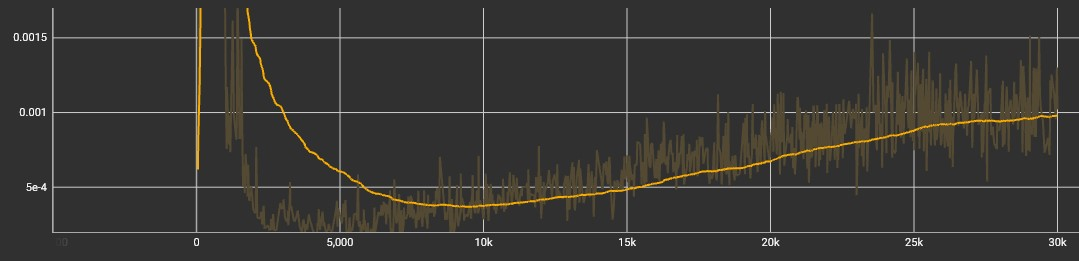
\includegraphics[width=1\linewidth]{pretrain-exp-reg.jpg}
            \caption{Tensorboard által generált grafikon az arckifejezés-regularizáció alakulásáról az előtanítás során.}
            \label{fig:pretrain-exp-reg}
        \end{figure}

        \begin{figure}[h!]	
            \centering
            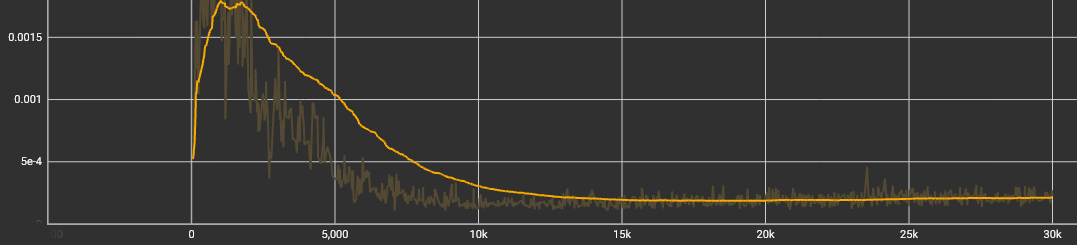
\includegraphics[width=1\linewidth]{pretrain-shape-reg.png}
            \caption{Tensorboard által generált grafikon az alak-regularizáció alakulásáról az előtanítás során.}
            \label{fig:pretrain-shape-reg}
        \end{figure}

        \begin{figure}[h!]	
            \centering
            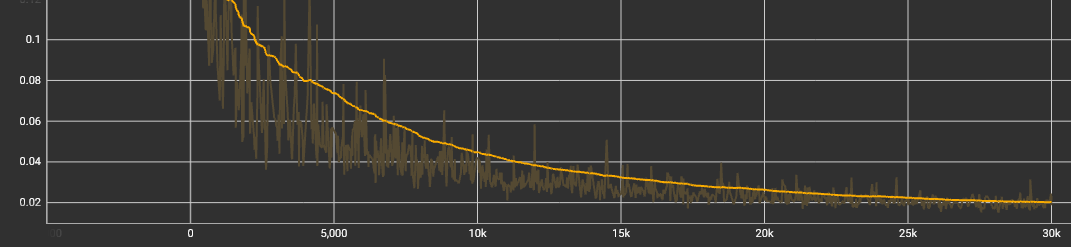
\includegraphics[width=1\linewidth]{pretrain-lmk-loss.png}
            \caption{Tensorboard által generált grafikon az arcpont reprojekciós veszteség alakulásáról az előtanítás során.}
            \label{fig:pretrain-lmk-loss}
        \end{figure}

        \begin{figure}[h!]	
            \centering
            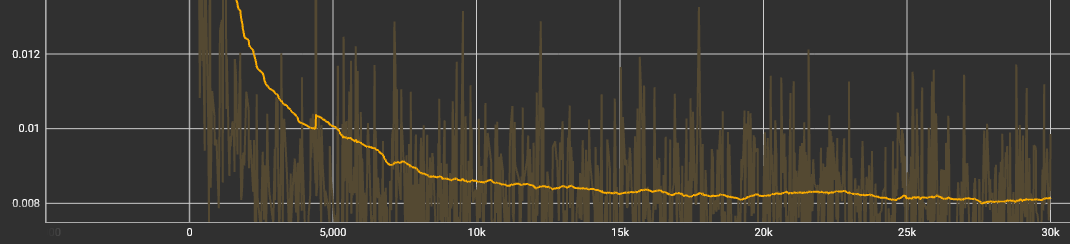
\includegraphics[width=1\linewidth]{pretrain-eye-loss.png}
            \caption{Tensorboard által generált grafikon a szemzárási veszteség alakulásáról az előtanítás során.}
            \label{fig:pretrain-eye-loss}
        \end{figure}

        \begin{figure}[h!]	
            \centering
            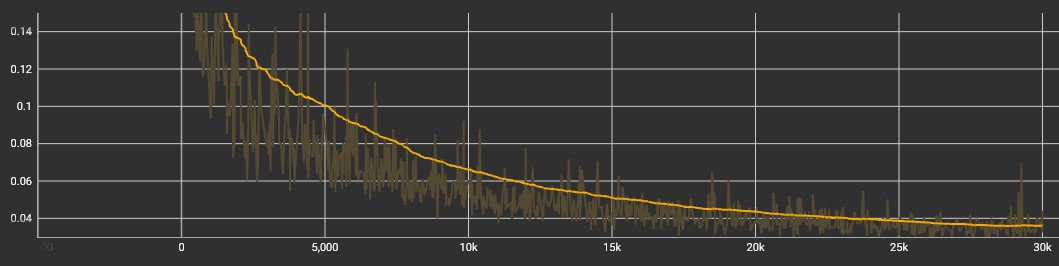
\includegraphics[width=1\linewidth]{pretrain-all-loss.jpg}
            \caption{Tensorboard által generált grafikon az összesített veszteség alakulásáról az előtanítás során.}
            \label{fig:pretrain-all-loss}
        \end{figure}

        \begin{figure}[h]	
            \centering
            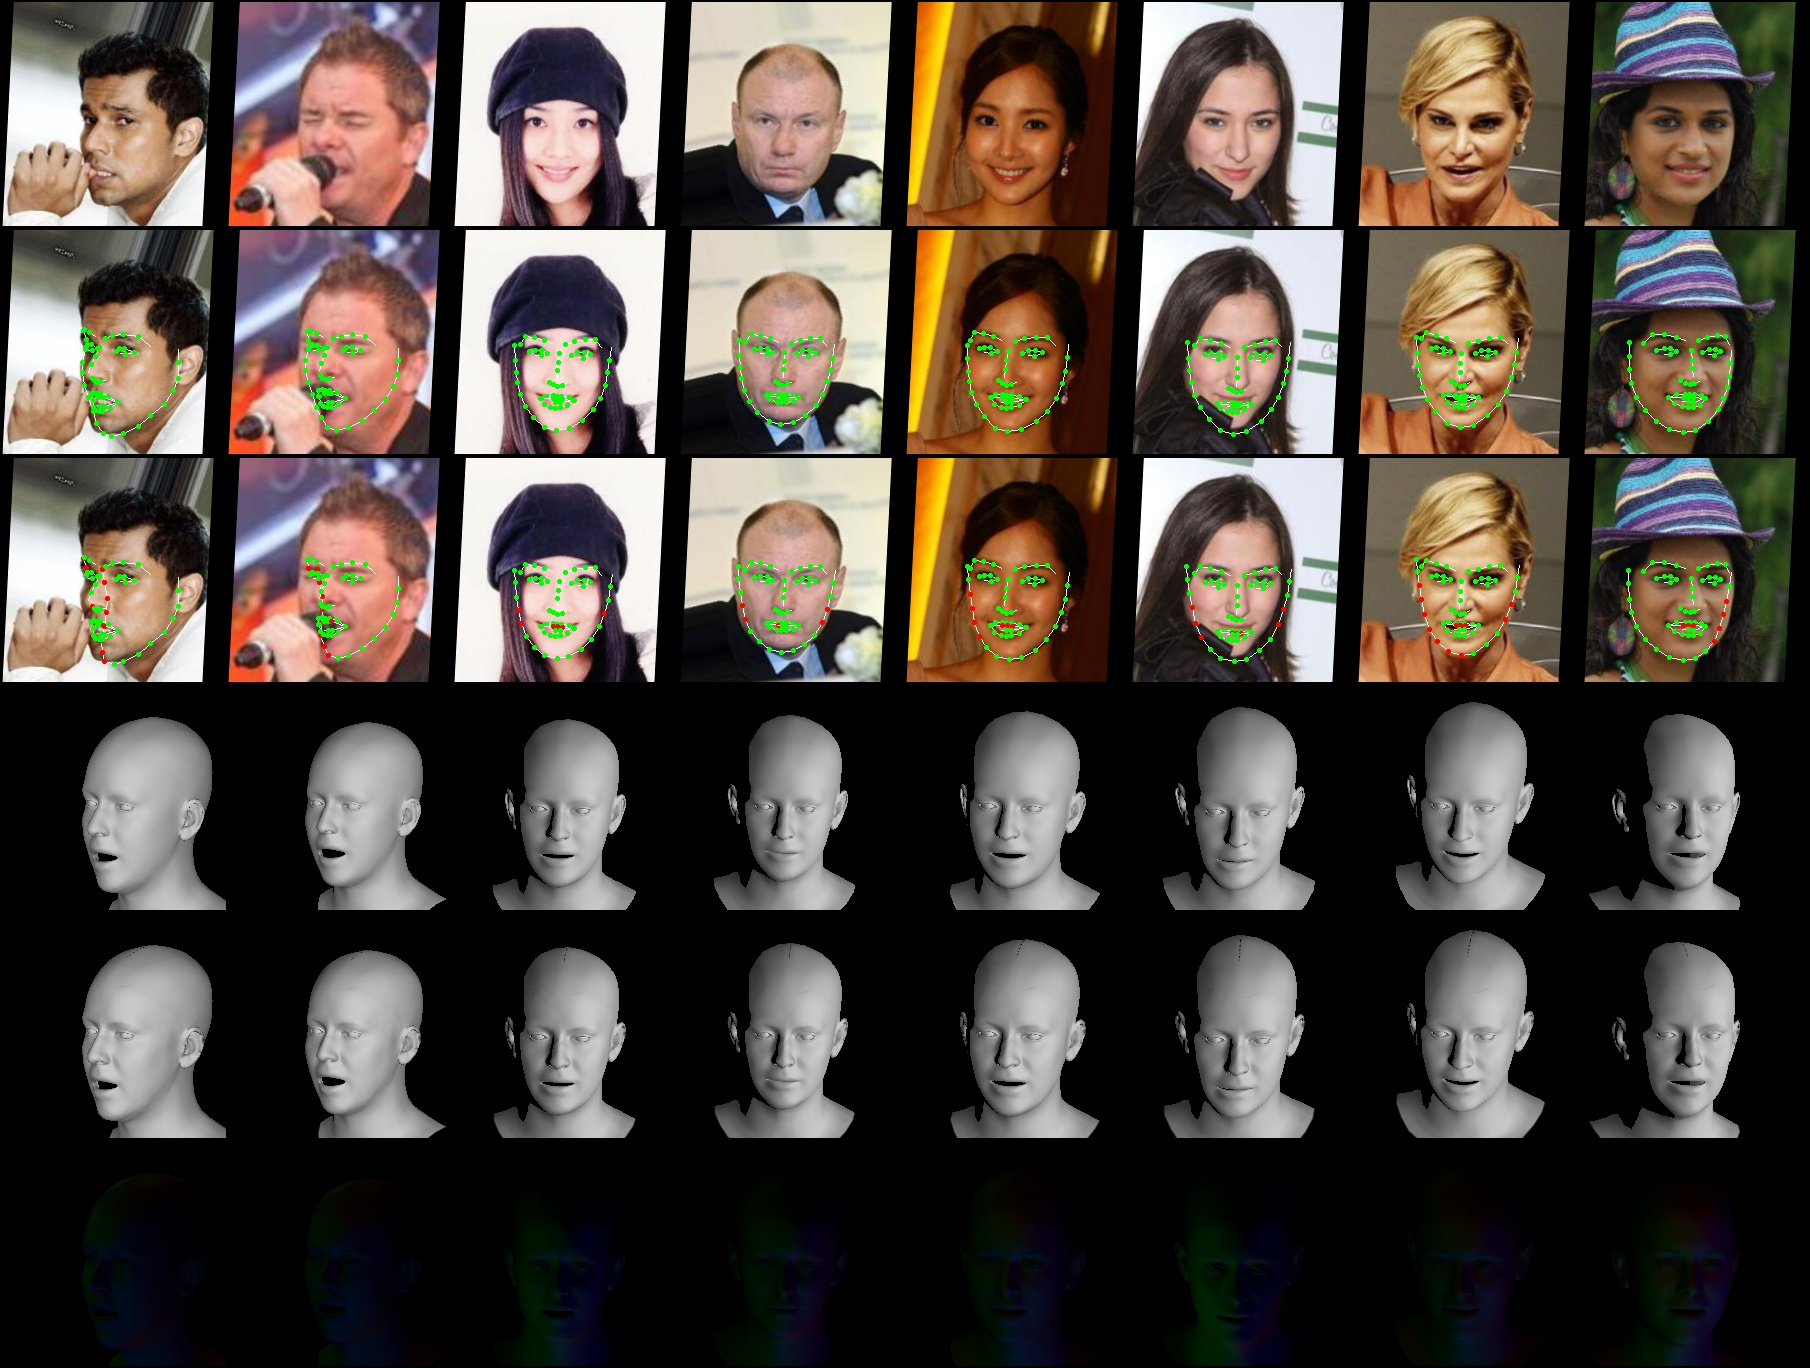
\includegraphics[width=1\linewidth]{pretrain-val-images.jpg}
            \caption{Az előtanítás végén készített rekonstrukciók a teszt halmazból kivett képekről.}
            \label{fig:pretrain-val-images}
        \end{figure}

        \clearpage
        A(z) \ref{fig:pretrain-exp-reg}.,\ref{fig:pretrain-shape-reg}., \ref{fig:pretrain-lmk-loss}., \ref{fig:pretrain-eye-loss}. és \ref{fig:pretrain-all-loss}. ábrák az előtanítás során Tensorboard által generált grafikonokat szemlélteti az egyes regularizációk és veszteségek alakulásáról.
        
        A(z) \ref{fig:pretrain-val-images}. ábrán az előtanítás végén készített rekonstrukciók láthatóak a teszthalmazból kivett képekről. Az első sorban a bemeneti képek, a másodikban az elvárt arcpontok, a harmadik sorban a hálózat által jósolt arcpontok találhatóak. A negyedik sor az elvárt arcpontok felhasználásával készített 3D-s fejmodelleket, az ötödik pedig a hálózat által megjósolt arcpontok felhasználásával készített fejmodelleket tartalmazza. A legalsó sorban a megjósolt fényviszonyok közötti alaptextúrával ellátott modell látható.
        
        \paragraph{Szegmentáló hálózat előtanítása}
        
        A modellt $10$ epochon vagy $135000$ iteráción keresztül 12-es kötegmérettel tanítjuk. Az U-Net modellünket az előtanítás során egy bináris képszegmentálási feladatra tanítjuk egy logaritmizált pixelenkénti bináris kereszt-entrópia veszteségfüggvényt (binary cross-entropy loss function with logits) és  Adadelta optimalizálót 0,03-as tanulási rátával használva.
        
        Ezenkívül van egy tanulási sebesség ütemező 5000-es lépésmérettel és 0,99-es gamma értékkel.

        Az előtanítás a következő lépésekből áll:
            \begin{enumerate}
                \item Az első lépés a tanulási képek és a szegmentációs maszkok betöltése és előfeldolgozása.

                \item Az U-Net modell inicializálása.

                \item Az U-Net modell betanítása a bináris kereszt-entrópia veszteségfüggvény és az Adam optimalizáló, illetve az ütemező segítségével.

                \item A modell elmentése.
            \end{enumerate}

        A bináris kereszt-entrópia veszteségfüggvényt általában bináris osztályozási problémákra, például képszegmentálásra használják. A veszteségfüggvény a megjósolt szegmentációs maszk és az alapigazság maszk közötti különbséget méri a kép minden egyes pixelére. A logaritmizált bináris kereszt-entrópia veszteségfüggvény  az U-Net modell kimenetét veszi, amely egy valós értékű tenzor, és a sigmoid aktivációs függvényt alkalmazza a valószínűségi térkép előállításához. A veszteségfüggvény ezt követően összehasonlítja ezt a valószínűségi térképet az alapigazság maszkjával, amely egy 0 és 1 értékeket tartalmazó bináris maszk, a veszteség kiszámításához.

        A logaritmizált bináris kereszt-entrópia veszteségfüggvényt előnyben részesítjük a hagyományos bináris kereszt-entrópia veszteségfüggvénnyel szemben, mivel képes kezelni azokat a numerikus instabilitási problémákat, amelyek a kis valószínűségek logaritmizálása során előfordulhatnak.

        Az Adadelta optimalizáló népszerű választás a mélytanulási feladatokhoz, különösen a nagy adathalmazokkal és ritka gradiensekkel rendelkező feladatokhoz. Ez egy adaptív tanulási sebesség optimalizáló algoritmus, amely a múltbeli gradiensek mozgó átlagát használja az egyes paraméterek tanulási sebességének beállításához. Ez hasznos lehet a zajos gradiensek és a különböző paraméterek eltérő nagyságú gradienseinek kezelésében.

        A mi esetünkben van még egy tanulási sebesség ütemező 5000-es lépésmérettel és 0,99-es gammaértékkel. Ez az ütemező minden lépésméret iterációnál a gamma tényezővel csökkenti a tanulási rátát. Ezt a technikát általában a mélytanulási modellek teljesítményének javítására használják a tanulási ráta idővel történő fokozatos csökkentésével, ami lehetővé teszi az optimalizáló számára, hogy egy jobb optimumra álljon be, és elkerülje annak túllövését.

        Az Adadelta optimalizáló és a tanulási sebesség ütemező kombinációja segíthet az U-Net modell hatékonyabb konvergálásában és a túlillesztés elkerülésében, különösen zajos vagy ritka adatok jelenlétében.
        
        Összességében az Adadelta és az Adam nagyon hasonló algoritmusok, amelyek hasonló körülmények között jól teljesítenek, részletesebben Sebastian Ruder \cite{ruder} munkájában lehet olvasni.
        \\

        \begin{wrapfigure}{l}{0.25\textwidth}
        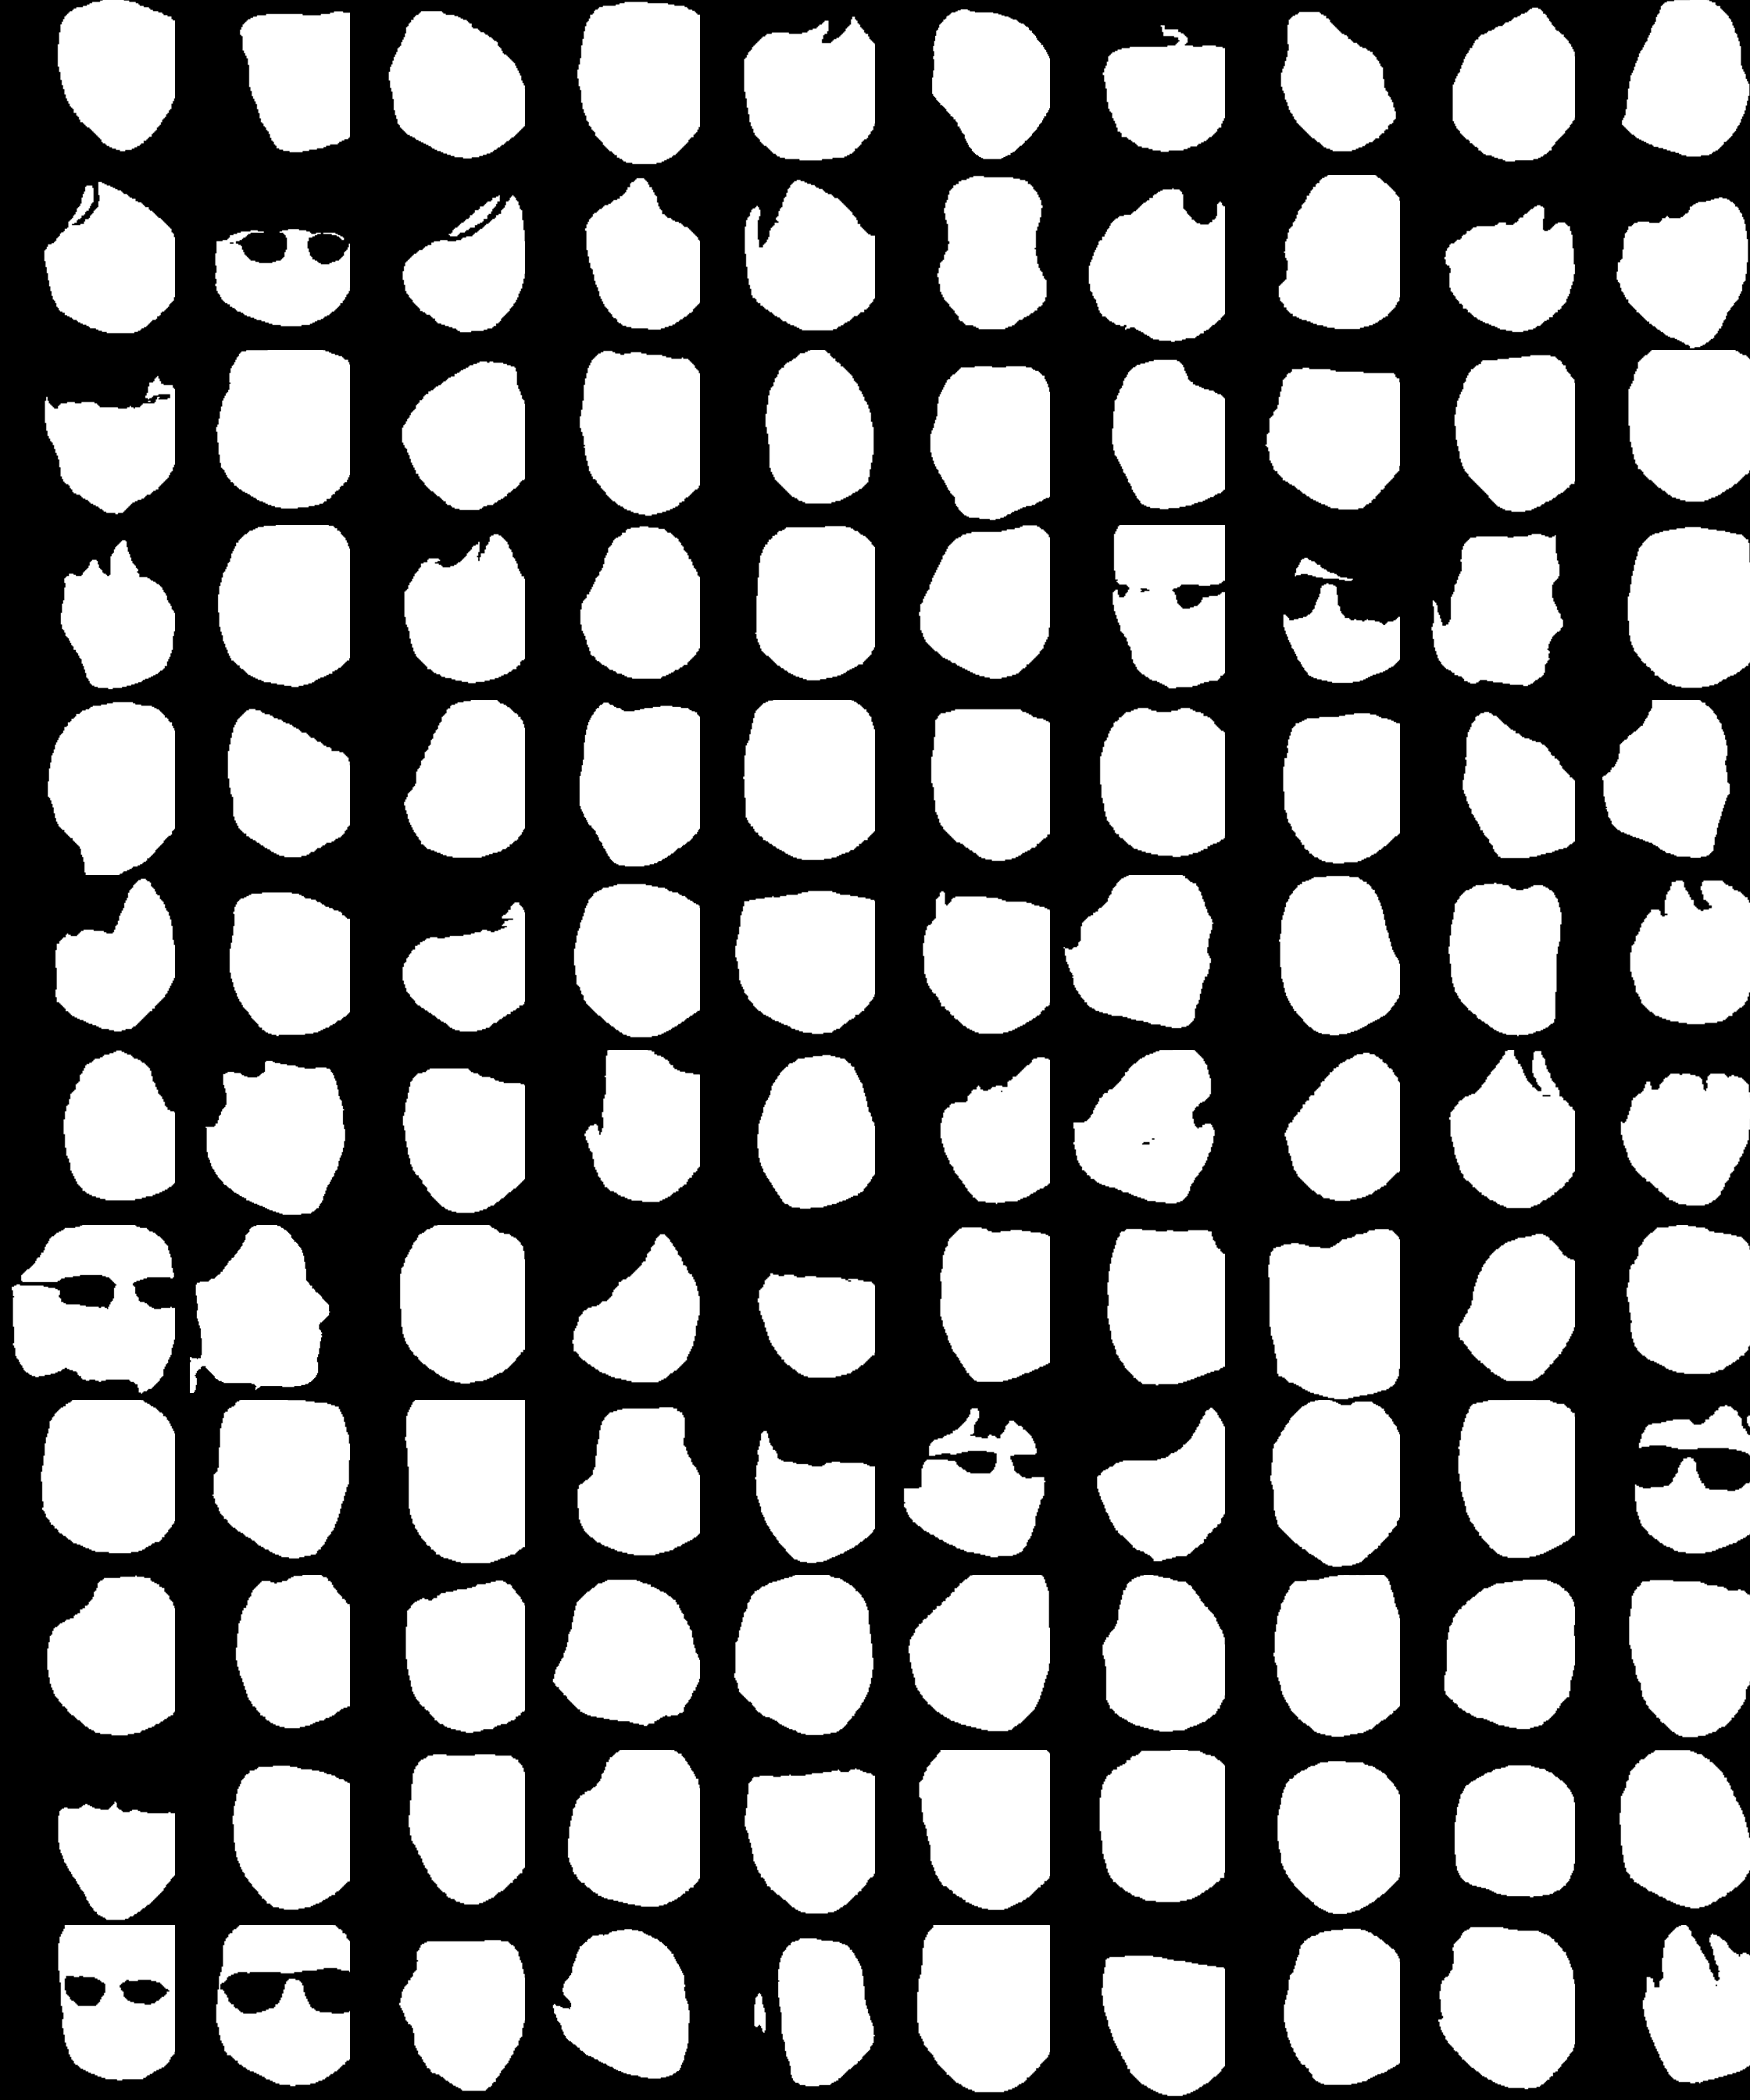
\includegraphics[width=0.9\linewidth]{test-masks-gt.png} 
        \caption{Az elvárt alapigazság maszkok.}
        \label{wrap-fig:gt-masks}
        \end{wrapfigure}

        \begin{figure}[h!]
          \centering
          \begin{minipage}[b]{0.4\textwidth}
            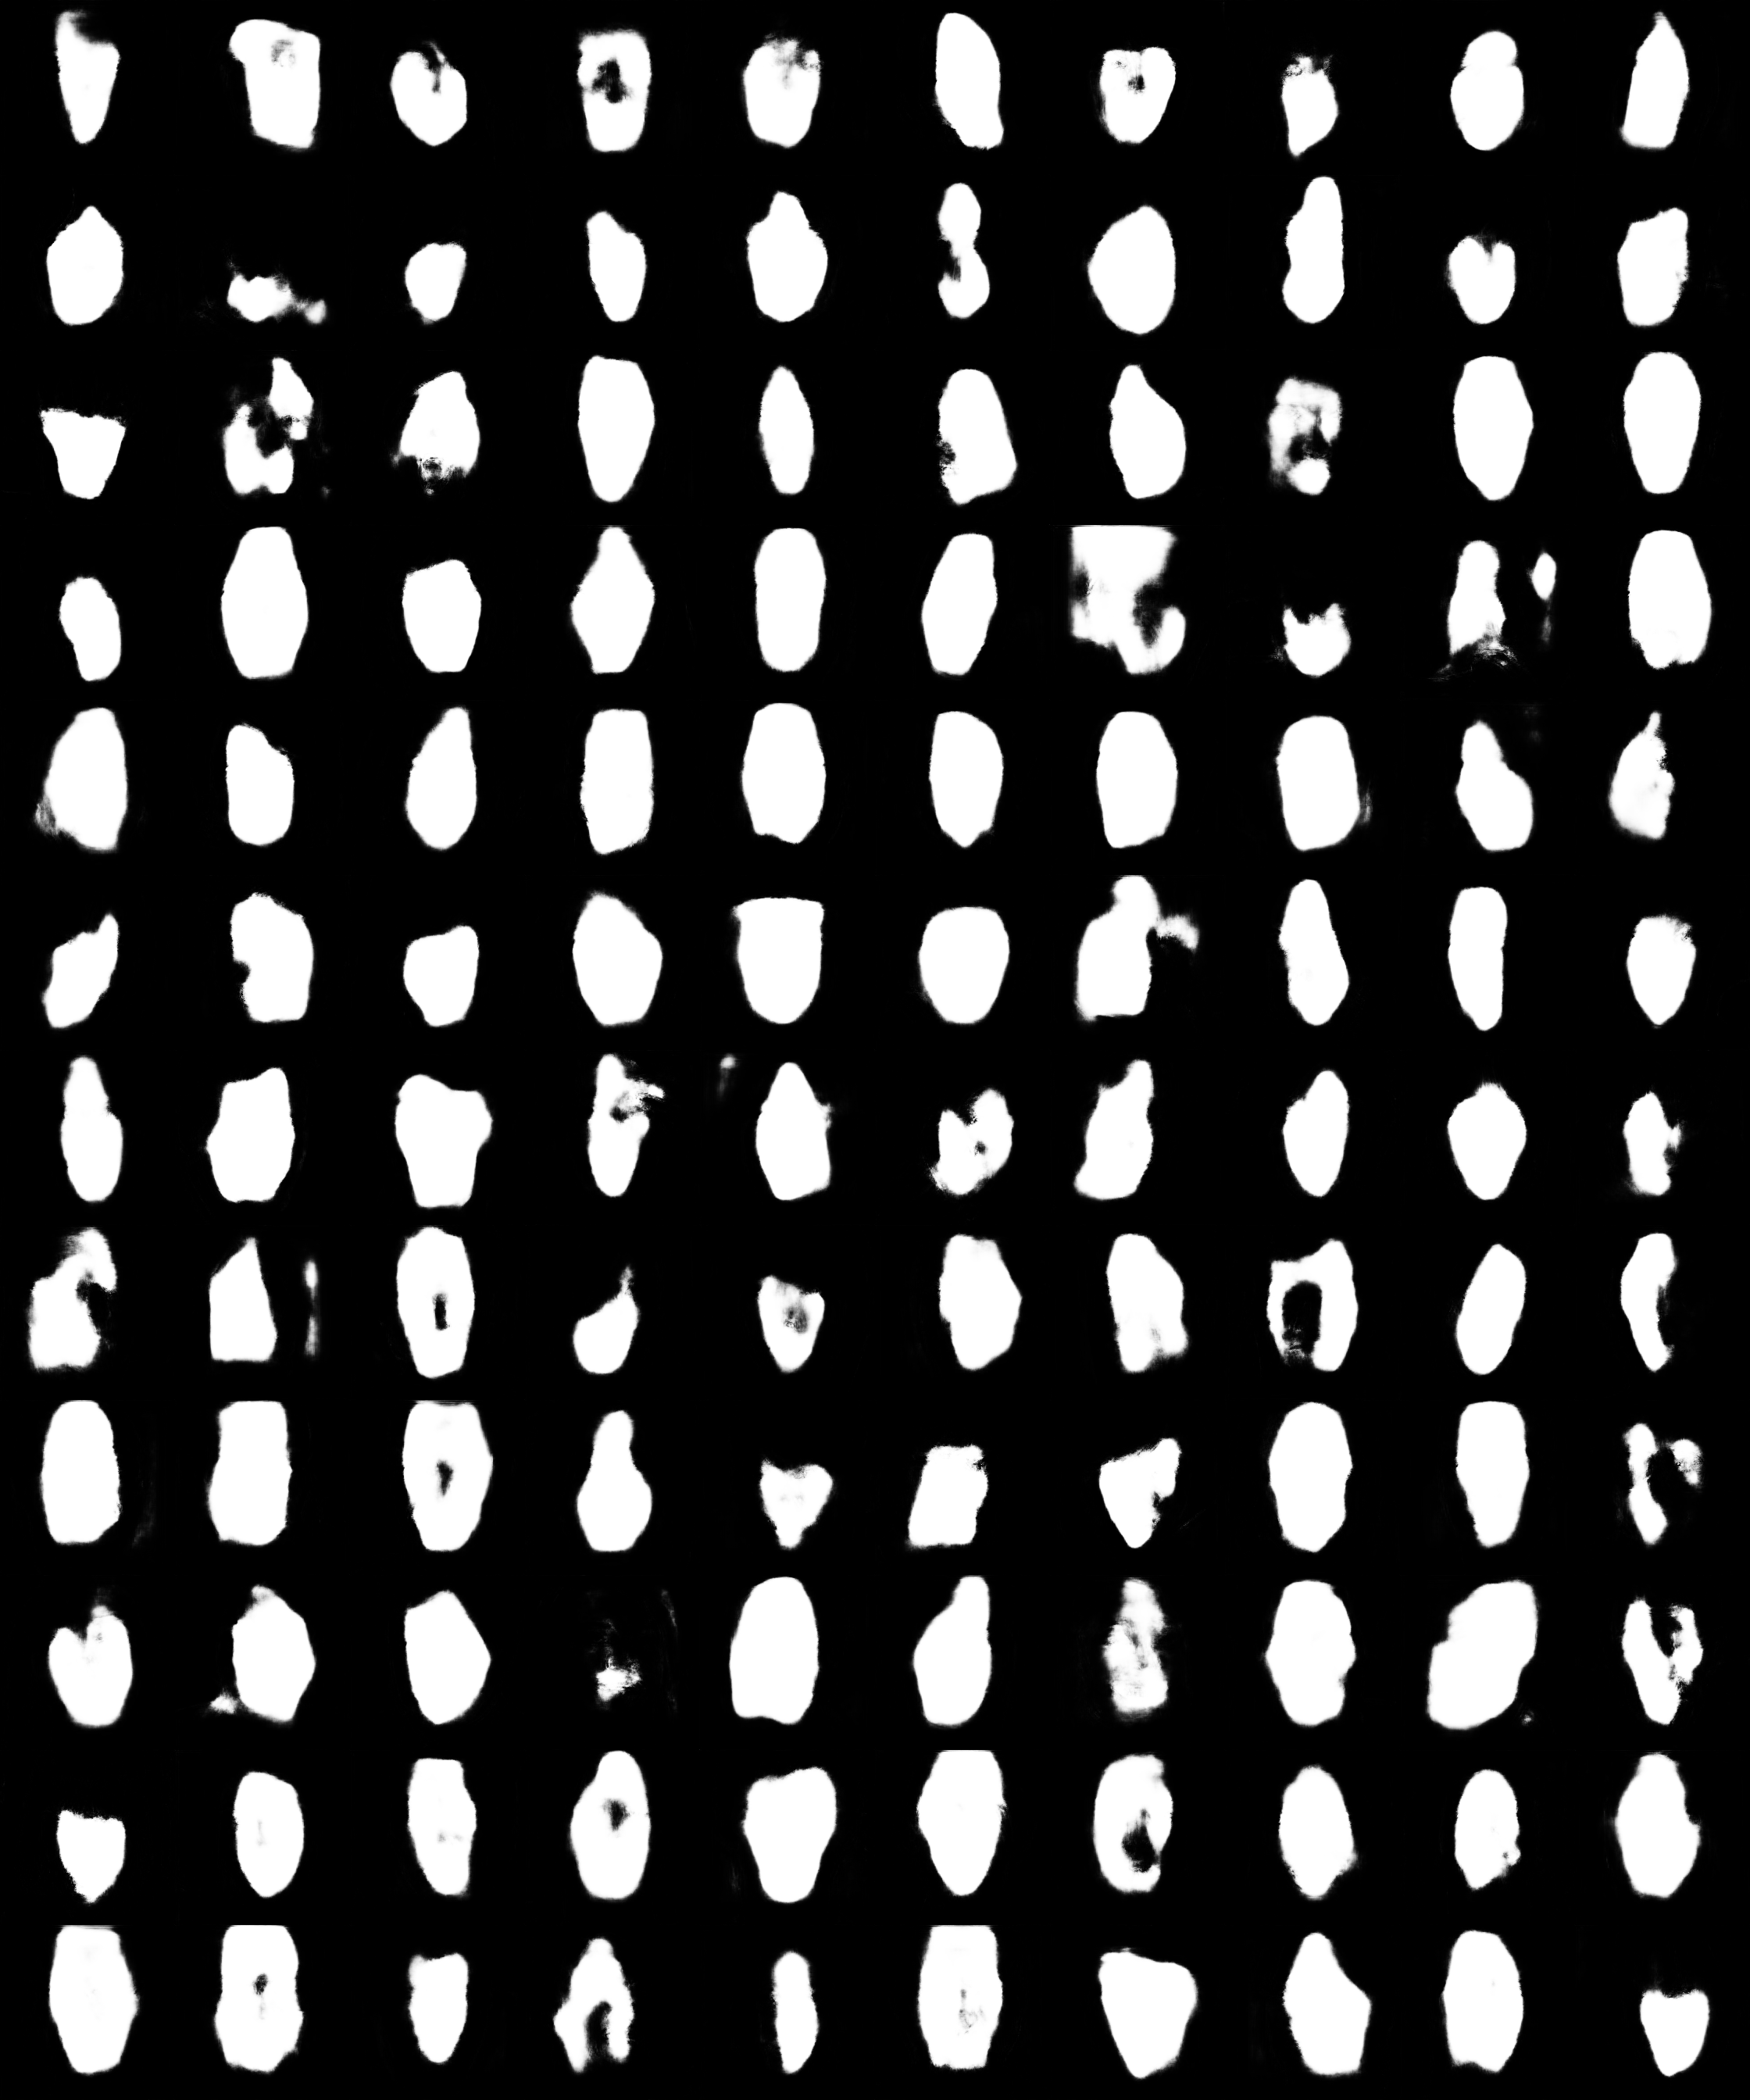
\includegraphics[width=\textwidth]{test-masks-1000.png}
            \caption{Generált maszkok 1000 iteráció után.}
            \label{fig:masks-1000it}
          \end{minipage}
          \hfill
          \begin{minipage}[b]{0.4\textwidth}
            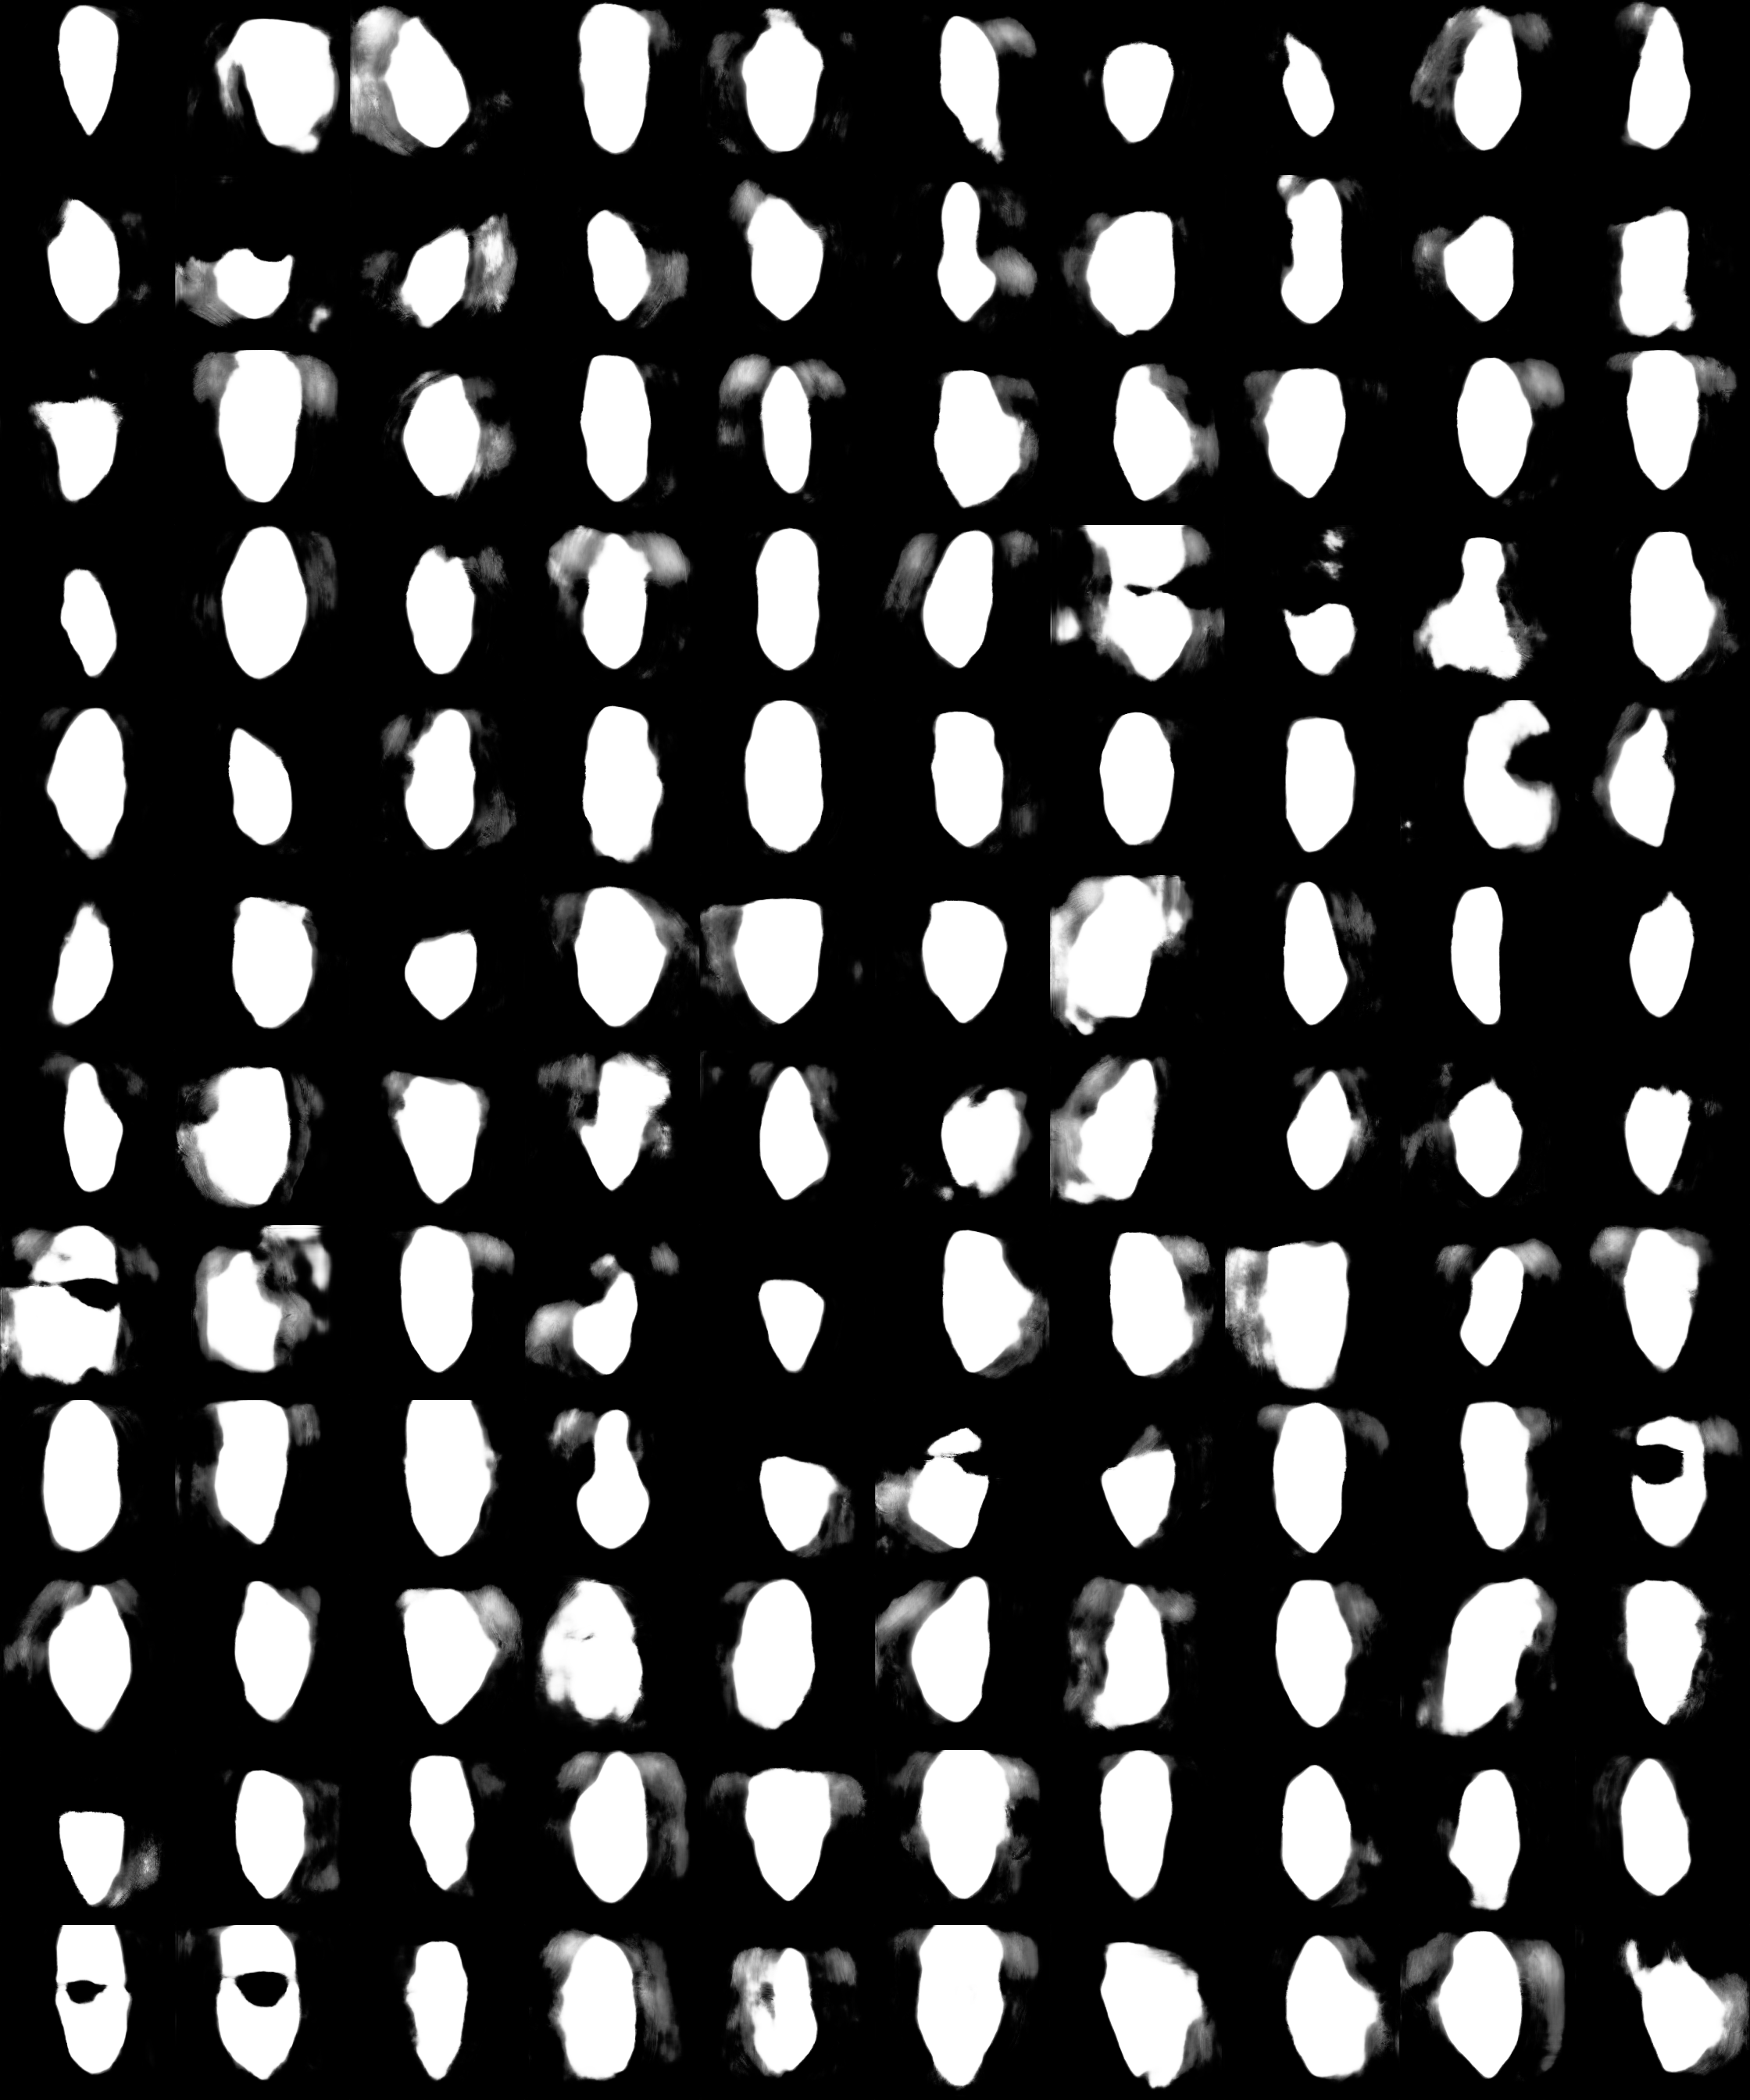
\includegraphics[width=\textwidth]{test-masks-30000.png}
            \caption{Generált maszkok 30000 iteráció után.}
            \label{fig:masks-30000it}
          \end{minipage}
          \begin{minipage}[b]{0.4\textwidth}
            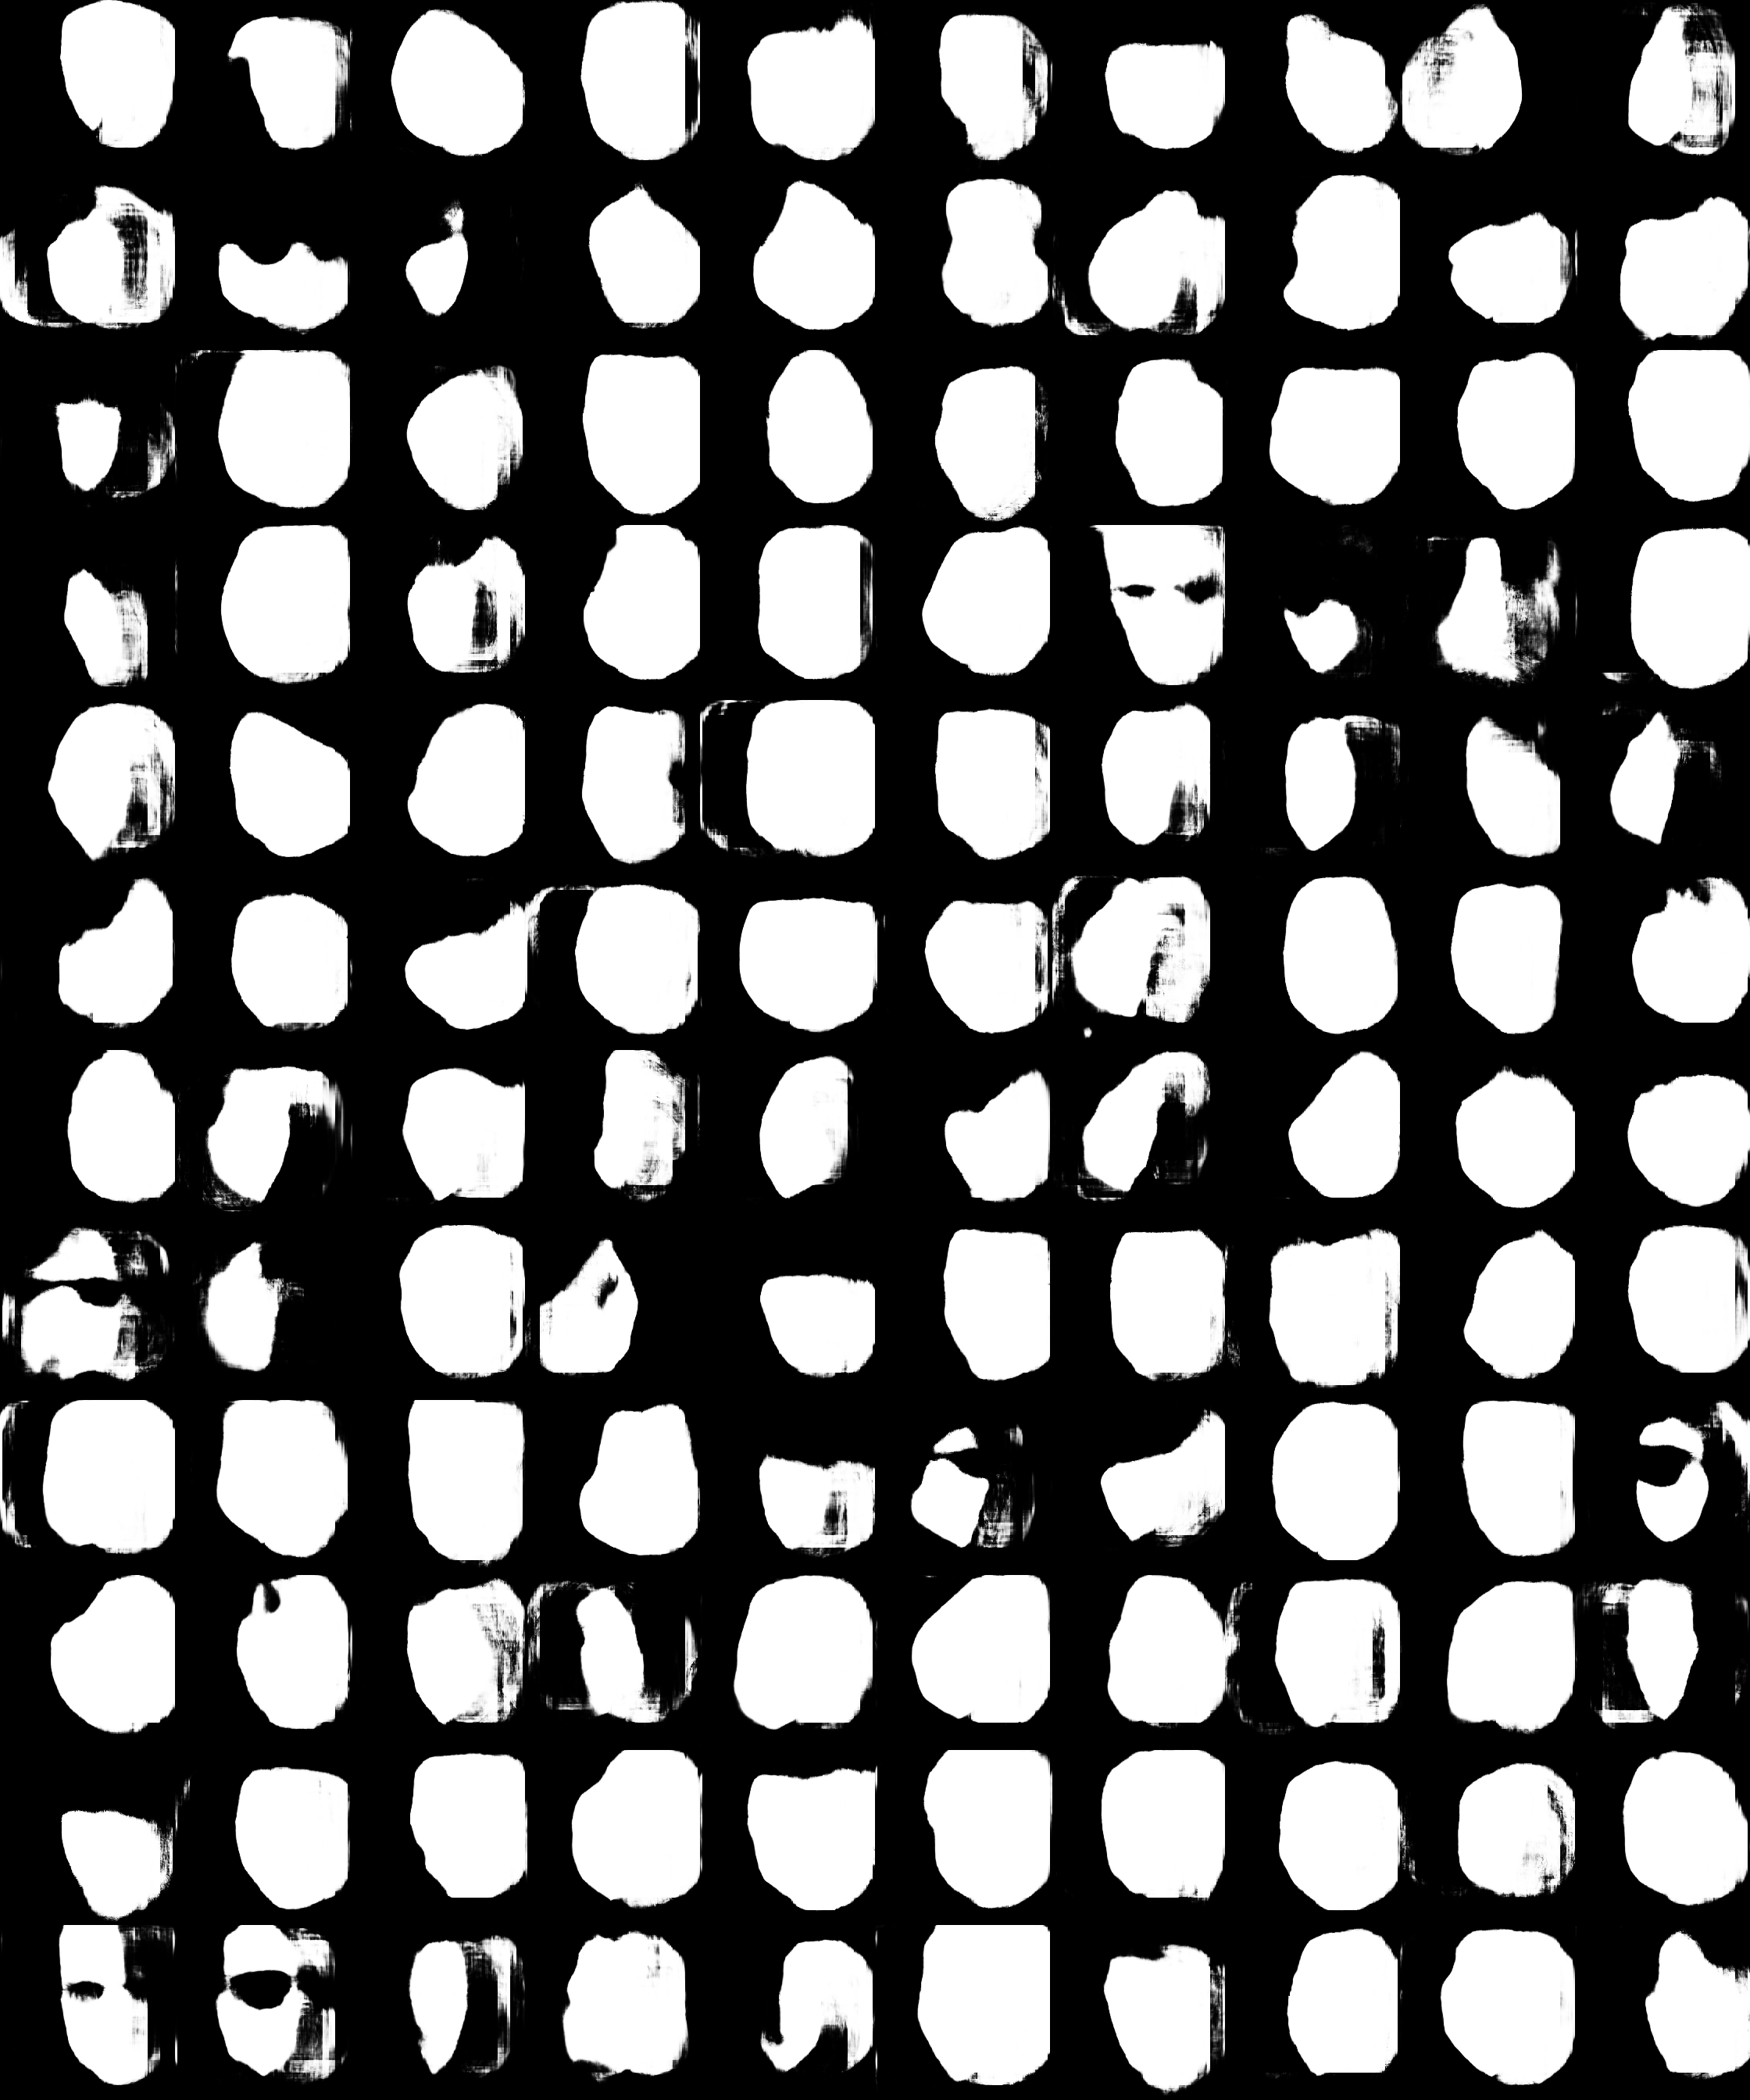
\includegraphics[width=\textwidth]{test-masks-90000.png}
            \caption{Generált maszkok 90000 iteráció után.}
            \label{fig:masks-90000it}
          \end{minipage}
          \hfill
          \begin{minipage}[b]{0.4\textwidth}
            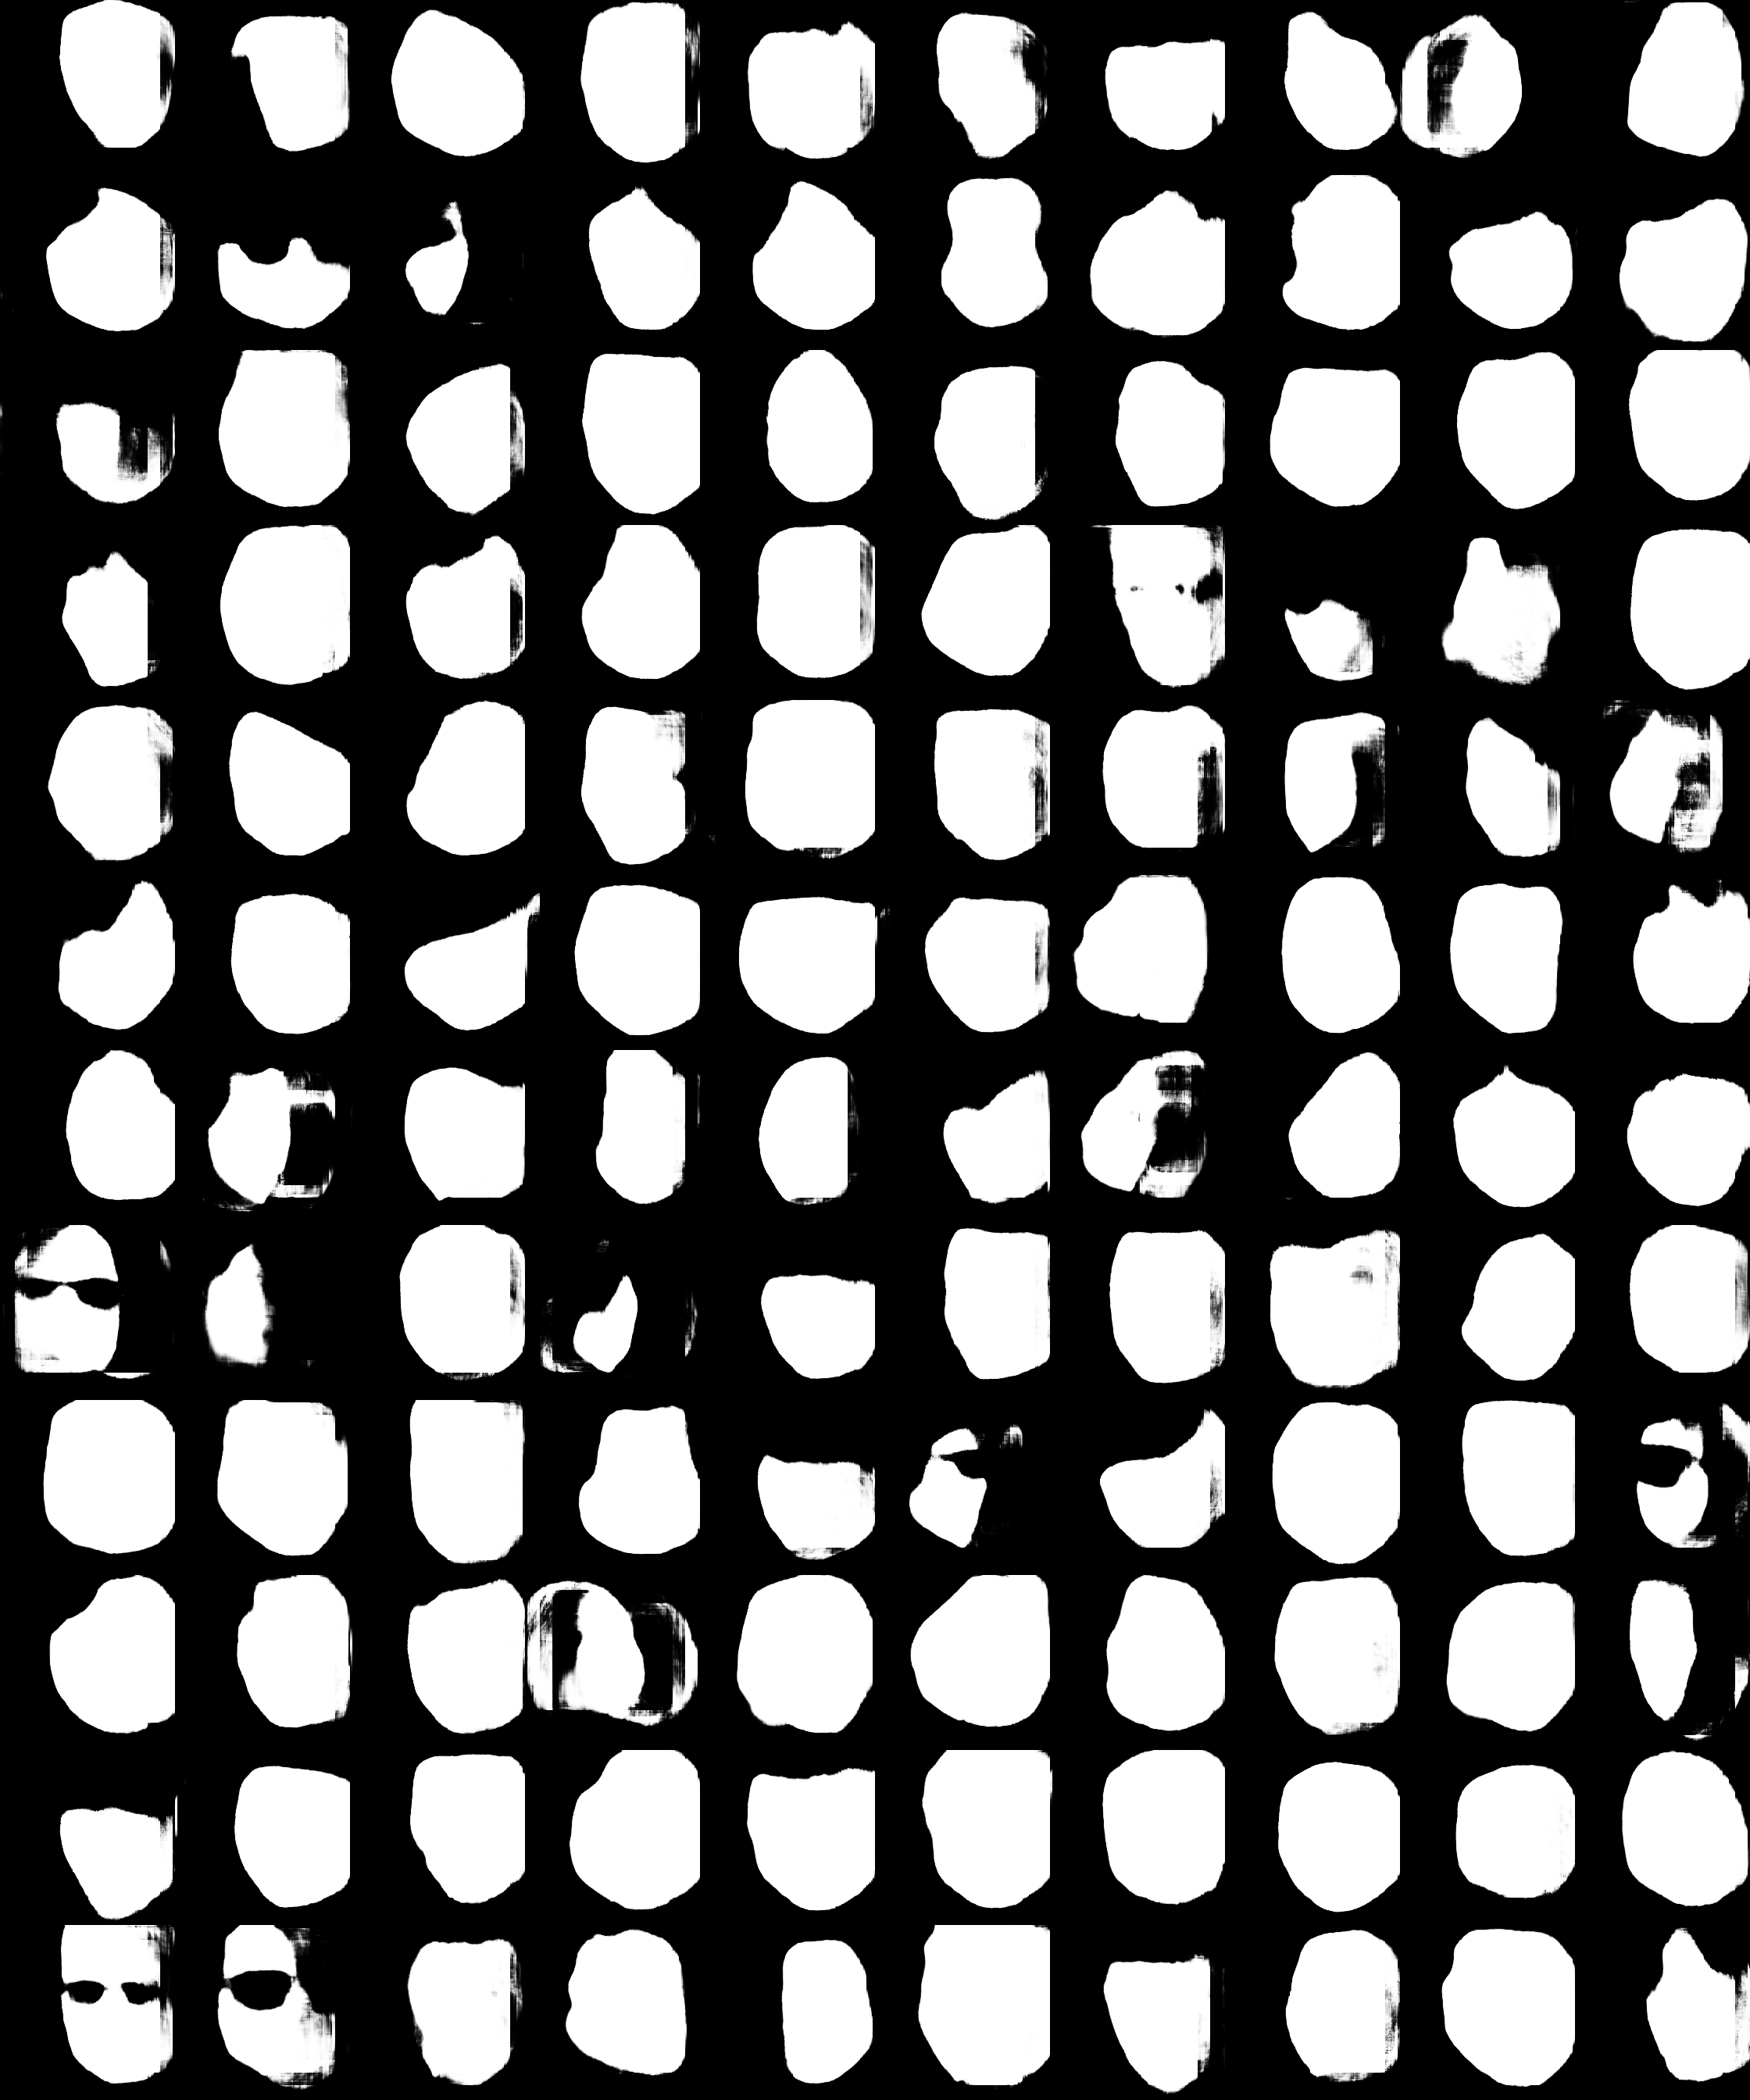
\includegraphics[width=\textwidth]{test-masks-135000.png}
            \caption{Generált maszkok 135000 iteráció után.}
            \label{fig:masks-135000it}
          \end{minipage}
          \caption{\centering A szegmentáló hálózat eredményei az előtanítás során}
          \label{fig:pretrain-mask}
        \end{figure}

        
        
        A(z) \ref{fig:pretrain-mask}. ábrán (\ref{fig:masks-1000it}. - \ref{fig:masks-135000it}. ábrák) a szegmentáló hálózat által generált arcmaszkok láthatóak az egyes lépésszámok után. A hálózat teszteléséhez a bemeneti képek a validációs adathalmazból kerülnek kiválasztásra. A validáció minden $1000$. lépésben lefut. Az elvárt alapigazság maszkok a(z) \ref{wrap-fig:gt-masks}. ábrán láthatóak. 

        \clearpage

        \paragraph{Hálózatok tanítása}

        Az arcrekonstrukciós és a szegmentáló hálózatot a FOCUS keretrendszeréből merítve várható érték maximalizációs (Expectation-Maximization/EM) módszerrel tanítottuk be.

        A(z) EM algoritmus egy széles körben használt iteratív optimalizálási módszer, amely különösen hasznos, amikor látens változókkal kapcsolatos modellekkel foglalkozunk, ahol az érintett változók egy része nem közvetlenül megfigyelhető, hanem a megfigyelt adatokból következtethetünk rájuk. A neurális hálózatok tanításával összefüggésben az EM-algoritmus olyan összetett problémák megoldására használható, ahol a mögöttes adateloszlás ismeretlen, vagy közvetlenül nem modellezhető a látens változók (azaz a nem megfigyelt változók) értékeinek váltakozó becslésével, és a becsült értékek alapján a hálózati paraméterek optimalizálásával.

        A 3D arc rekonstrukció és az arcmaszk szegmentálása esetén az EM algoritmus használható a két feladat együttes, felváltva történő betanítására. Az ötlet lényege, hogy először a 3D arcgeometriát becsüljük meg a bemeneti képből egy 3D rekonstrukciós hálózat segítségével, majd a becsült 3D geometria segítségével irányítjuk az arcmaszk szegmentálását a képen. A szegmentálási feladatot egy külön hálózat, egy U-háló segítségével végezzük el, amelyet a bemeneti képen lévő arctartomány bináris maszkjának előrejelzésére tanítunk be.

        Az EM-algoritmus két fő lépés között váltakozik: az E-lépés és az M-lépés. Az E-lépésben a látens változók (azaz a 3D arcgeometria) becslése a megfigyelt adatok (azaz a bemeneti kép) és a hálózati paraméterek aktuális becslése alapján történik. Az M-lépésben a hálózati paraméterek frissítése a látens változók becsült értékei alapján történik. Ez a folyamat a konvergenciáig ismétlődik, azaz addig, amíg a látens változók és a hálózati paraméterek becsült értékei nem változnak jelentősen az iterációk között.

        A szegmentáló hálózat tanítása során az arcrekonstrukciós hálózat paraméterei nem változnak, valamint a rekonstrukciós hálózat tanítása során a szegmentáló hálózat súlyai rögzítettek.

        Az arcrekonstrukciós hálózat tanítási lépésének átadásra kerül a szegmentáló hálózat által megjósolt arcmaszk, illetve a szegmentáló hálózat tanítási lépésének az arcrekonstrukciós hálózat által elkészített raszterizált 2D-s képet adjuk át.

        A két hálót összesen $5$ epochon vagy $150000$ iteráción keresztül tanítottuk be $4$-es kötegszámmal. Minden $6000$ lépésből $5000$ lépésben az arcrekonstrukciós modellt és $1000$ lépésben a szegmentációs modellt tanítottuk. Az arcrekonstrukciós hálózat tanítása során az Adam optimalizálót használtuk $1e-4$ tanulási rátával, míg a szegmentáló hálózatnál az Adadelta optimalizálót $0.03$-as tanulási rátával használtuk.
        A szegmentáló hálózathoz egy tanulási sebesség ütemezőt használtunk $5000$-es lépésmérettel és $0.99$-es gamma értékkel. A képméret $224 \times 224$.

        Az arcrekonstrukciós hálózat tanítása során az alábbi veszteségfüggvényeket használjuk a hozzájuk tartozó súlyértékekkel:
        \begin{itemize}
            \item Arckifejezés regularizáció ($E_{\psi}$) $\lambda_{E_{\psi}} = 1e - 4$ súlyértékkel.
            
            \item Alak regularizáció ($E_{\beta}$) $\lambda_{E_{\beta}} = 1e - 4$
            
            \item Fény regularizáció ($E_{l}$) $\lambda_{l} = 1$ súlyértékkel.
            
            \item Albedó/textúra regularizáció ($E_{\alpha}$) $\lambda_{E_{\alpha}} = 1e-4$ súlyértékkel.
            
            \item Arcpont reprojekciós veszteségfüggvény ($L_{lmk}$)
            $\lambda_{L_{lmk}} = 1$ súlyértékkel.
            
            \item Identitás veszteségfüggvény ($L_{id}$)
            $\lambda_{L_{id}} = 0.2$ súlyértékkel.
            
            \item Szemzárási veszteségfüggvény ($L_{eye}$)
            $\lambda_{L_{eye}} = 1$ súlyértékkel.
            
            \item Fotometriai veszteségfüggvény ($L_{pho}$)
            $\lambda_{L_{pho}} = 2$ súlyértékkel.
        
        \end{itemize}

        A szegmentáló hálózat tanításához a(z) \ref{unetseg}. fejezetben definiált veszteségfüggvényeket használjuk fel.

        \begin{figure}[h!]
            \centering
            \begin{subfigure}[b]{0.55\textwidth}
               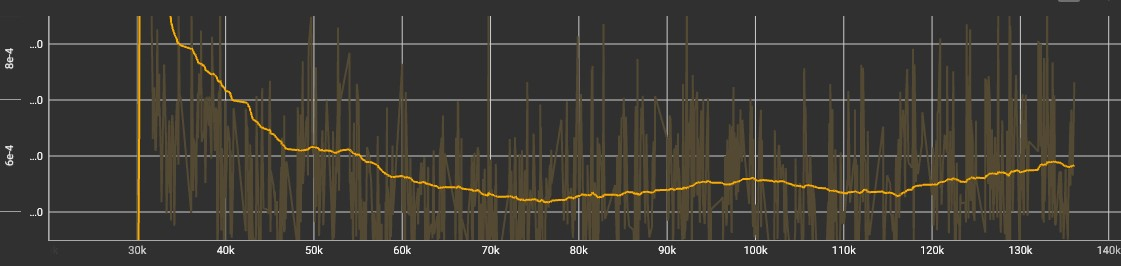
\includegraphics[width=1\linewidth]{coarse-shape-reg.jpg}
               \caption{Alak regularizáció }
               \label{fig:coarse-shape-reg} 
            \end{subfigure}
            
            \begin{subfigure}[b]{0.55\textwidth}
               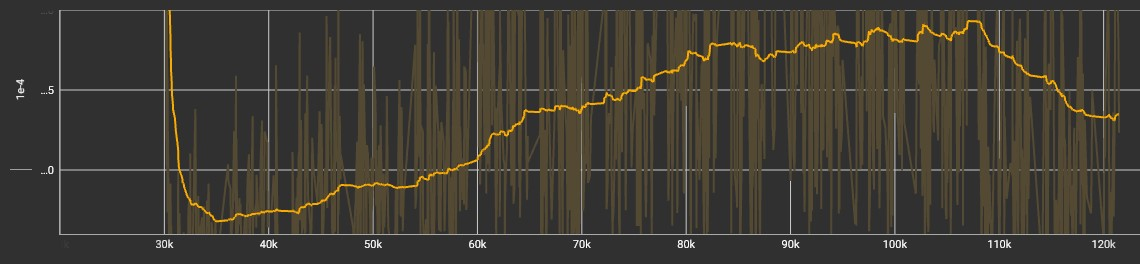
\includegraphics[width=1\linewidth]{coarse-light-reg.jpg}
               \caption{Fény regularizáció}
               \label{fig:coarse-light-reg} 
            \end{subfigure}

            \begin{subfigure}[b]{0.55\textwidth}
               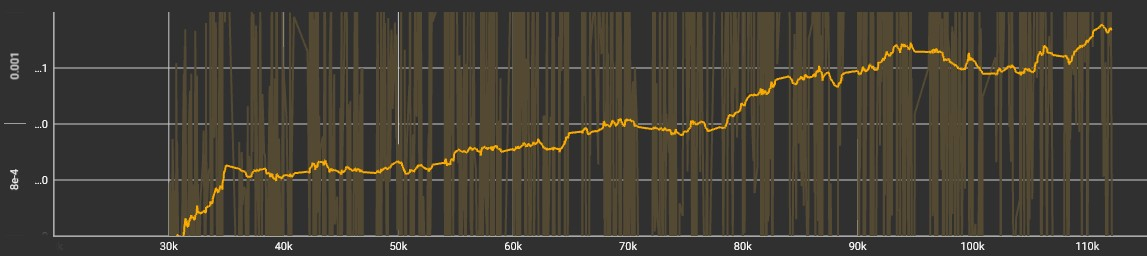
\includegraphics[width=1\linewidth]{coarse-exp-reg.jpg}
               \caption{Arckifejezés regularizáció}
               \label{fig:coarse-exp-reg} 
            \end{subfigure}

            \begin{subfigure}[b]{0.55\textwidth}
               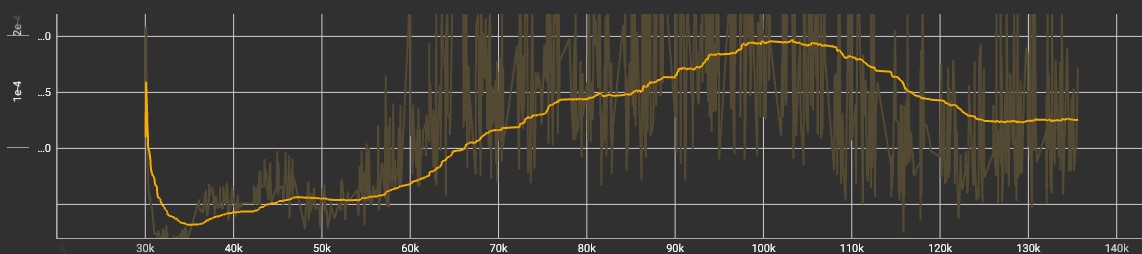
\includegraphics[width=1\linewidth]{coarse-tex-reg.jpg}
               \caption{Albedó regularizáció}
               \label{fig:coarse-tex-reg} 
            \end{subfigure}
            \caption{Az arcrekonstrukciós hálózat regularizációnak alakulása a tanítás során. Minden grafikonon az X tengely jelöli a lépésszámot, az Y pedig az egyes lépésszámoknál felvett értékek láthatóak.}
            \label{fig:coarse-reg-results}
        \end{figure}
        \begin{figure}[h!]
            \centering
            \begin{subfigure}[b]{0.55\textwidth}
               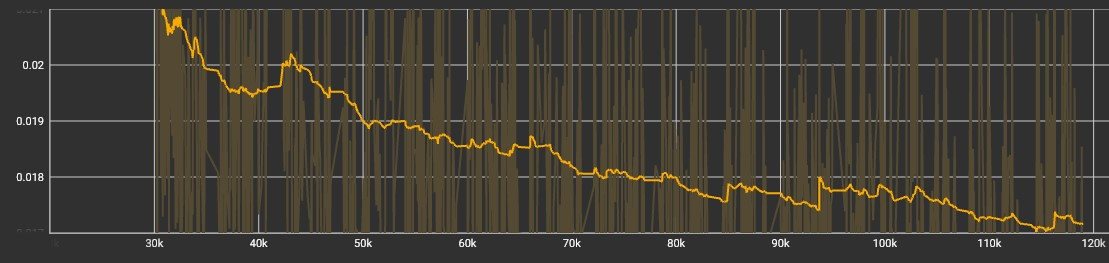
\includegraphics[width=1\linewidth]{coarse-lmk-loss.jpg}
               \caption{Arcpont reprojekciós veszteség}
               \label{fig:coarse-lmk-loss} 
            \end{subfigure}

            \begin{subfigure}[b]{0.55\textwidth}
               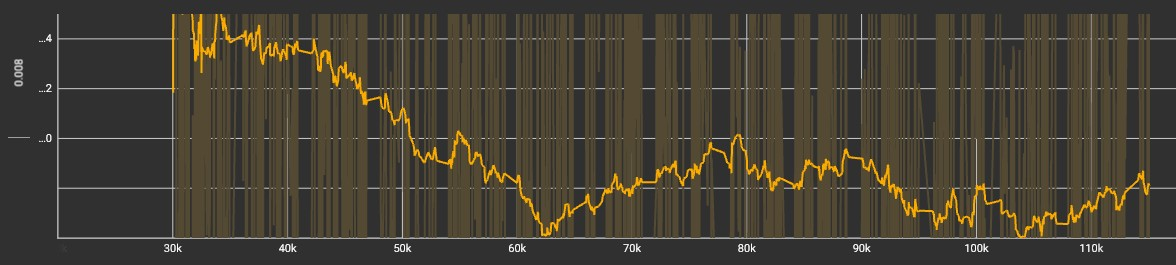
\includegraphics[width=1\linewidth]{coarse-eye-loss.jpg}
               \caption{Szemzárási veszteség}
               \label{fig:coarse-eye-loss} 
            \end{subfigure}

            \begin{subfigure}[b]{0.55\textwidth}
               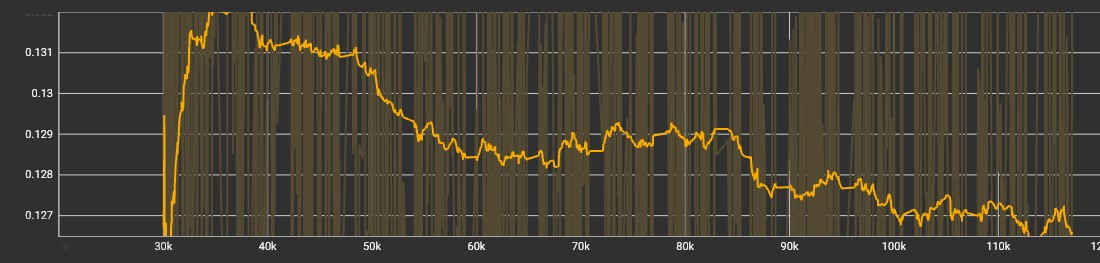
\includegraphics[width=1\linewidth]{coarse-identity-loss.jpg}
               \caption{Identitás veszteség}
               \label{fig:coarse-identity-loss} 
            \end{subfigure}

            \begin{subfigure}[b]{0.55\textwidth}
               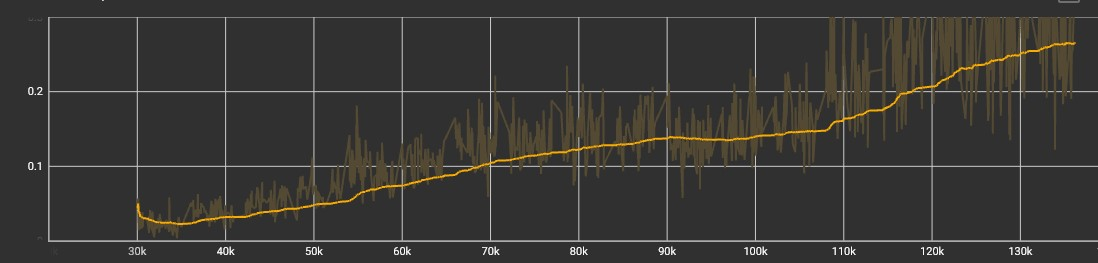
\includegraphics[width=1\linewidth]{coarse-pho-loss.jpg}
               \caption{Fotometriai veszteség}
               \label{fig:coarse-pho-loss} 
            \end{subfigure}

            \begin{subfigure}[b]{0.55\textwidth}
               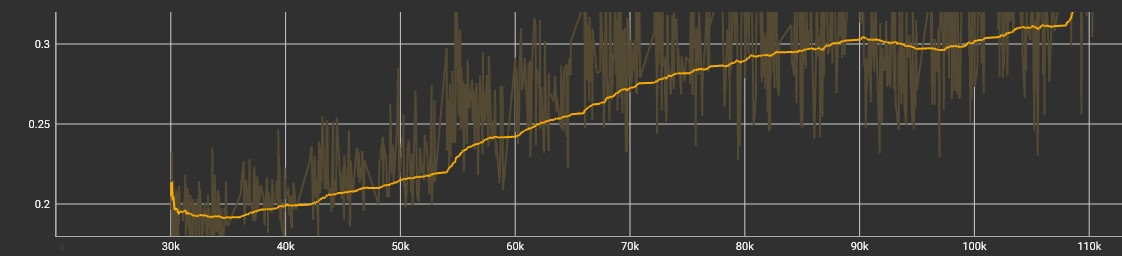
\includegraphics[width=1\linewidth]{coarse-all-loss.jpg}
               \caption{Összesített arcrekonstrukciós veszteség}
               \label{fig:coarse-all-loss} 
            \end{subfigure}
            \caption{Az arcrekonstrukciós hálózat veszteségeinek alakulása a tanítás során. Minden grafikonon az X tengely jelöli a lépésszámot, az Y pedig az egyes lépésszámoknál felvett értékek láthatóak.}
            \label{fig:coarse-loss-results}
        \end{figure}\clearpage

        A(z) \ref{fig:coarse-reg-results}. és a(z) \ref{fig:coarse-loss-results}. ábrákon a rekonstrukciós hálózat tanítása során kiszámításra került regularizációk és veszteségek láthatók. Az arckifejezés regularizáció és a fotometriai veszteség növekedése annak tudható be, hogy a DECA-tól eltérően mi nem használtunk több arcképet személyenként különböző arckifejezésekkel és pózokkal. Ugyanebből az okból kifolyólag csak a(z) \ref{facepretrainsec}. fejezetben említett költségfüggvényeket használtuk fel a tanítás során.

        \begin{figure}[h!]	
            \centering
            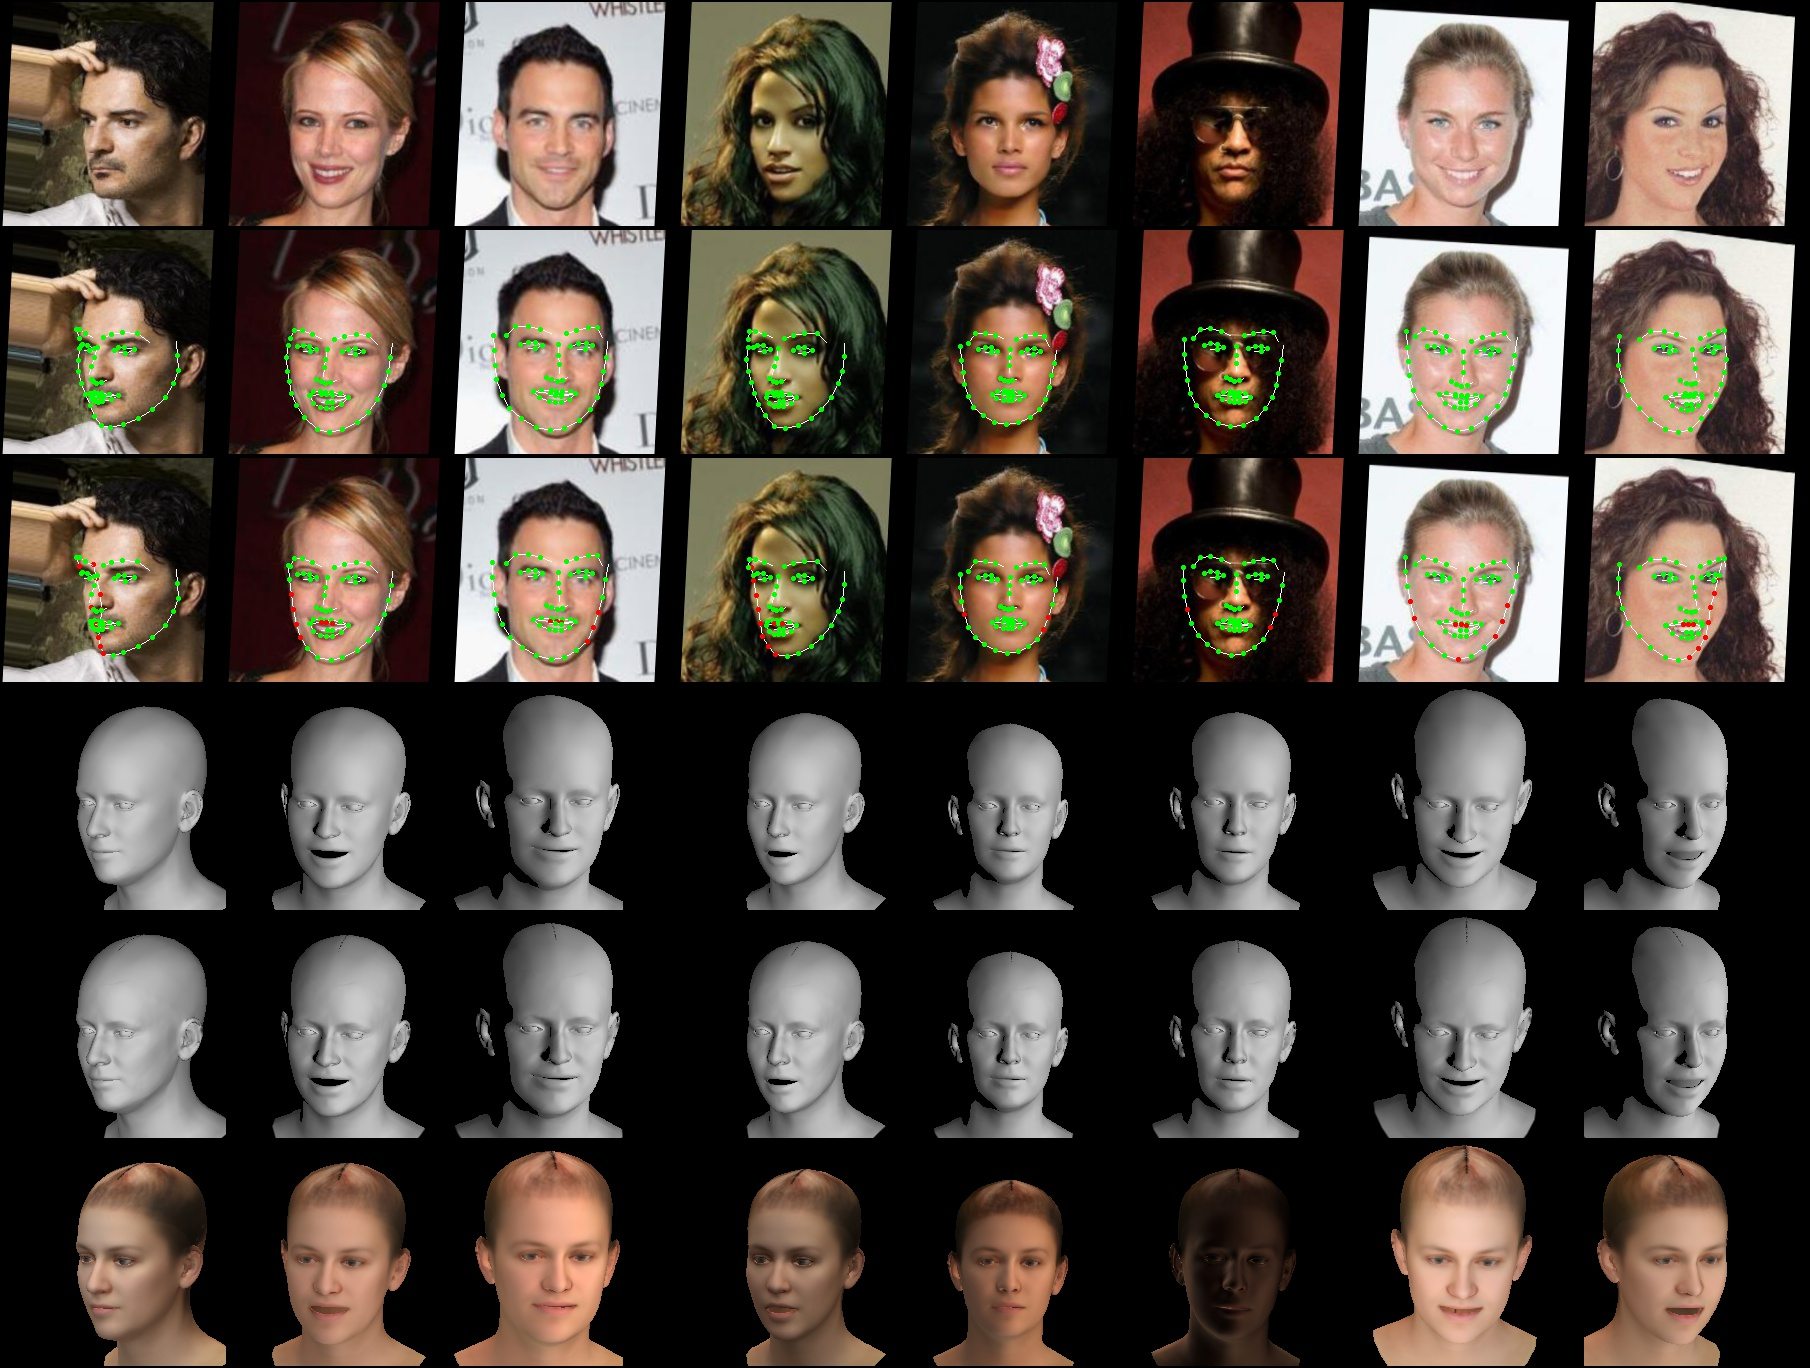
\includegraphics[width=1\linewidth]{coarse-val-image.jpg}
            \caption{A tanítás végén készített rekonstrukciók a teszthalmazból kivett képekről.}
            \label{fig:coarse-val-images}
        \end{figure}
        
        A(z) \ref{fig:coarse-val-images}. ábrán a tanítás végén készített rekonstrukciók láthatóak a teszthalmazból kivett képekről. Az első sorban a bemeneti képek, a másodikban az elvárt arcpontok, a harmadik sorban a hálózat által jósolt arcpontok találhatóak. A negyedik sor az elvárt arcpontok felhasználásával készített 3D-s fejmodelleket, az ötödik pedig a hálózat által megjósolt arcpontok felhasználásával készített fejmodelleket tartalmazza. A legalsó sorban a megjósolt fényviszonyok közötti alaptextúrával ellátott modell látható.

        A tanítás közben minden $500$. lépésben teszt rekonstrukciókat készítettünk a teszt adathalmazban szereplő képekről. A tesztelés előtt a hálózat súlyait rögzítettük.
        
          \begin{figure}[h!]
            \centering
            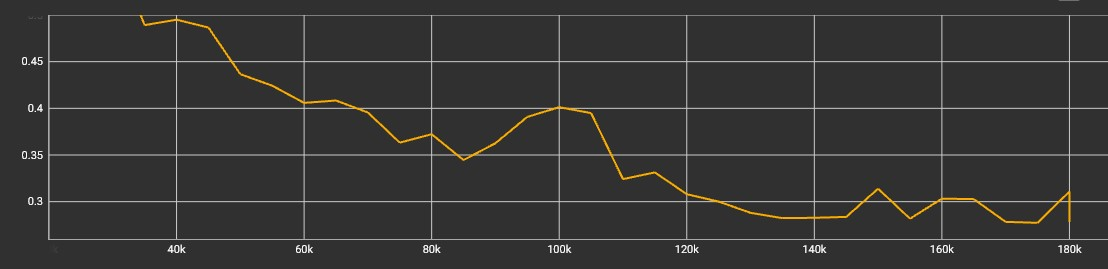
\includegraphics[width=1\linewidth]{coarse-unet-all-loss.jpg}
            \label{fig:coarse-unet-all-loss} 
            \caption{A szegmentáló hálózat összesített veszteségének alakulása a tanítás során. A grafikonon az X tengely jelöli a lépésszámot, az Y pedig az egyes lépésszámoknál felvett értékek láthatóak.}
            \label{fig:coarse-unet-loss-results}
        \end{figure}

        A(z) \ref{fig:coarse-unet-loss-results}. ábrán a szegmentáló hálózat összesített veszteségének alakulása látható a tanítás során.
        
                
        
        
    \subsubsection{Fontosabb felhasznált fájlok}

    Az alábbi fájlok nélkülözhetetlenek a kiváló minőségű 3D arcmodell rendereléséhez a FLAME modell segítségével:
    \begin{itemize}
        \item A \textit{head\_template.obj} fájl tartalmazza a FLAME modell sablonhálóját. A sablonháló egy átlagos arcformát reprezentál, és a személyre szabott 3D arcmodellek létrehozásának alapjául szolgál.
        
        \item A \textit{texture\_data\_256.npy} fájl tartalmazza a FLAME modell textúrainformációit. A textúrainformáció tartalmazza a bőr, a haj és a szemek színét és mintázatát.
        
        \item A \textit{fixed\_displacement\_256.npy}  fájl a FLAME modell elmozdulási adatait tartalmazza. Az elmozdulási információ határozza meg, hogyan kell deformálni a sablonhálót a személyre szabott 3D arcforma létrehozásához.
        
        \item A(z) \textit{uv\_face\_mask.png} fájl egy maszkot tartalmaz, amely meghatározza, hogy az arc mely régiói felelnek meg az UV textúratérképnek. Az UV textúratérkép egy 2D-s kép, amely a textúraadatokból a 3D-s arcmodellbe történő textúrainformáció átvitelére szolgál.
        
        \item A(z) \textit{uv\_face\_eye\_mask.png} fájl egy maszkot tartalmaz, amely meghatározza, hogy az arc mely régiói felelnek meg a szemeknek az UV textúratérképen. A szemrégiókat a textúraátvitel során külön kezeli a rendszer, hogy a szemtextúra megfelelően igazodjon.
        
        \item A \textit{mean\_texture.jpg} fájl a FLAME modell átlagos textúráját tartalmazza. Az átlagos textúra kiindulópontként szolgál a személyre szabott textúrák létrehozásához.

        \item A \textit{generic\_model.pkl} fájl egy előre betanított FLAME modellt tartalmaz, amely 3D-s arcmodellek létrehozására használható. Az előre betanított modell tartalmazza az alak, az arckifejezés és a póz paramétereit.

        \item A \textit{landmark\_embedding.npy} fájl tartalmazza a FLAME-modell tájékozódási pontjainak beágyazódását. A tájékozódási pontok beágyazása a 3D arcmodell 2D-s arc tájékozódási pont detektorral való összehangolására szolgál.

        \item A \textit{FLAME\_albedo\_from\_BFM.npz} fájl tartalmazza a FLAME modell albedóinformációit. Az albedóinformációk a 3D arcmodell bőrszínének és textúrájának létrehozásához használhatóak. Mivel a FLAME nem rendelkezik saját megjelenési modellel, ezért a BFM albedóinformációi kerülnek átalakításra, hogy kompatibilis legyen a FLAME-mel.
        
    \end{itemize}

    A DECA alapján az identitásveszteség kiszámításához egy előtanított arcfelismerő modellt használunk. Az előtanított modell súlyai a \textit{resnet50\_ft\_weight.pkl} fájlban vannak tárolva és a \url{https://github.com/cydonia999/VGGFace2-pytorch} oldalon érhető el.
    A modellt a VGGFace2 nevű nagyméretű arcfelismerési adathalmazon tanították elő.

    \subsubsection{Tanítási környezet}

        Az érzelemfelismerő és a nemfelismerő hálózatokat AMD Ryzen 3 1300X Quad-Core CPU @ 3.50GHz processzorral, 16,0 GB DDR4 RAM és NVIDIA GeForce RTX 3060 12GB GDDR6 videókártyával rendelkező számítógépen tanítottuk, illetve fejlesztettük.
    
    \section{Eredmények}
 	      \subsection{Arcanalízis}

            Az érzelem felismerő rendszerünk teljesítményét összesen 7178 képpel értékeltük ki, amelyeket a tanítás során nem használtunk fel.

            \begin{table}[htb] 
                \begin{tabular}{lllll}
                \textbf{Érzelem}     & \textbf{Pontosság} (\%) & \textbf{Fedés} (\%) & \textbf{F1-mutató} (\%) & \textbf{Képek száma} (db) \\
                mérges      & 51             & 69               & 59             & 958              \\
                undor       & 80             & 44               & 57             & 111              \\
                félelem     & 59             & 34               & 43             & 1024             \\
                boldog      & 85             & 90               & 87             & 1774             \\
                semleges    & 69             & 56               & 62             & 1233             \\
                szomorú     & 53             & 63               & 57             & 1247             \\
                meglepődött & 78             & 80               & 79             & 831             \\
                \\
                találati arány  &    &   & 67    & 7178 \\
                makroátlag  &68    &62   & 63    & 7178 \\
                súlyozott átlag  &67    &67   & 66    & 7178 \\
                \end{tabular}
                \caption{Az egyes arckifejezések felismerésére elért eredmények.}
                \label{fig:fec-result-table}
            \end{table}

            A(z) \ref{fig:fec-result-table}. táblázat szemlélteti az egyes arckifejezések felismerésére elért eredményeinket.
            
            \begin{table}[htb] 
                
                \begin{tabular}{lll}
                \textbf{Elvárt érték} & \textbf{Becsült érték} & \textbf{Eredmény}      \\
                pozitív      & pozitív       & valós pozitív (TP) \\
                negatív      & negatív       & valós negatív (TN) \\
                negatív      & pozitív       & álpozitív (FP)     \\
                pozitív      & negatív       & álnegatív (FN)    
                \end{tabular}
                \caption{Eredmények típusai}
                \label{fig:cf-result-types}
            \end{table}

            
            Elvárt és becsült érték alapján négy féle eredmény határozható meg. Ezeket a(z) \ref{fig:cf-result-types}. táblázat szemlélteti. 
            
            A pontosság (P) azt méri, hogy az összes előre jelzett pozitív eredmény mekkora része volt ténylegesen pozitív. A pontosság a következő képpen számítható ki:

            \begin{equation}
                P = \frac{TP}{TP + FP}
            \end{equation}
            
            Az felidézés (F) azt méri, hogy a pozitív rekordok mekkora hányadát sikerült helyesen megjósolni. Formálisan:

            \begin{equation}
                F = \frac{TP}{TP + FN}
            \end{equation}
            
            Az F1-mutató a pontosság és a felidézés harmonikus átlaga, amely kiszámítható, mint:

            \begin{equation}
                F1 = \frac{2 \cdot P \cdot F}{P + F}
            \end{equation}
            
            A makroátlag a címkénkénti súlyozatlan átlagot, a súlyozott átlag pedig a címkénkénti képtámogatással súlyozott átlagot méri.            
        
            A nemek klasszifikálására 97\%-os, míg az érzelmek klasszifikálására 67\%-os találati arányt tudtunk elérni.
    
                \begin{figure}[h!]	
            		\centering
            		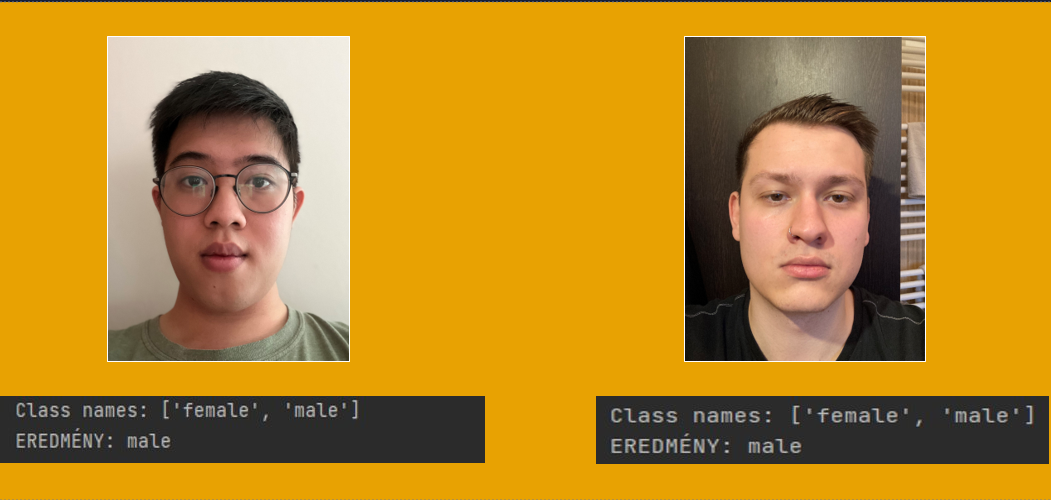
\includegraphics[width=1\linewidth]{gender}
                    \caption{  A nemek klasszifikálására készült hálózat becslései.}
                    \label{fig:gender}
            	\end{figure}
            
                A(z) \ref{fig:gender}. ábrán láthatjuk a modellünk által becsült nemeket.
            
                \begin{figure}[h!]	
            		\centering
            		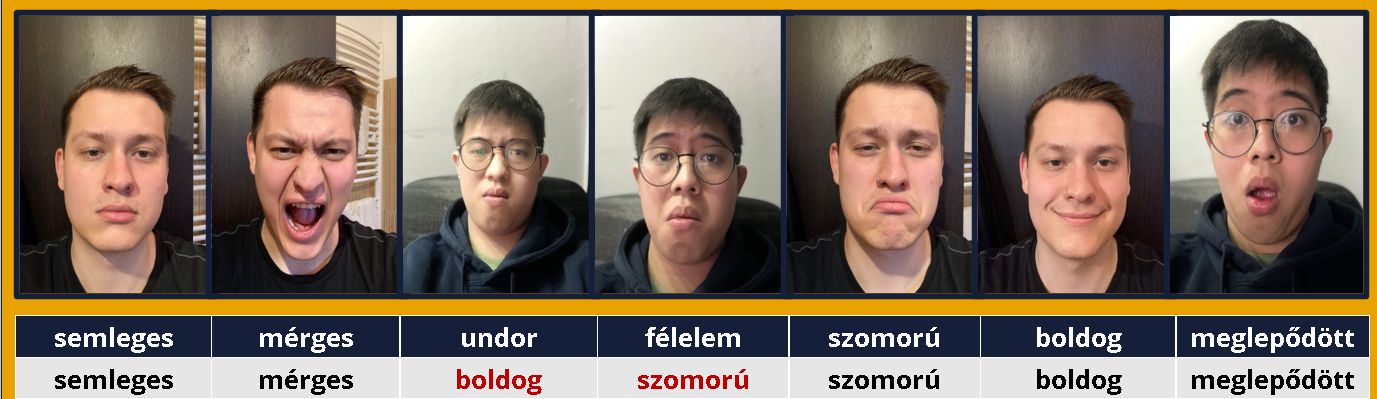
\includegraphics[width=1\linewidth]{arcanalizis}
                    \caption{  Az arckifejezések klasszifikálására készült hálózat becslései.}
                    \label{fig:expr}
            	\end{figure}
            
                A(z) \ref{fig:expr}. ábrán 7 különböző arckifejezésre láthatjuk a becsléseket és a hozzájuk tartozó elvárt eredményeket. Hogy pontosan lássuk a modell milyen kifejezésekre milyen pontossággal ad becslést, készítettünk egy konfuziós mátrixot, amely a(z) \ref{fig:cfmatrix}. ábrán látható.

                A konfúziós mátrix X tengelye az elvárt eredményt, míg Y tengelye a becsült eredményt jelöli.
                A mátrix segítségével megállapítható, hogy a rendszerünk a félelmet, a haragot és a szomorúságot gyakran összetéveszti egymással. Ugyan ez figyelhető meg a(z) \ref{fig:expr}. ábrán is. A 
                
            
                \begin{figure}[h!]	
            		\centering
            		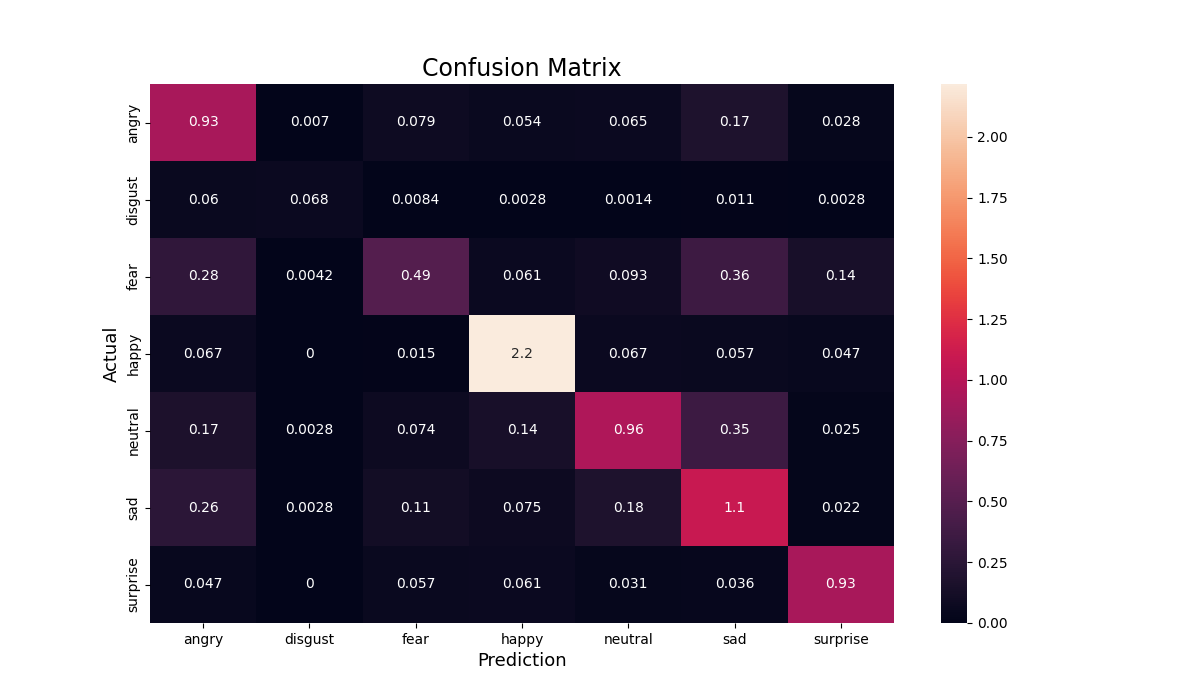
\includegraphics[width=1\linewidth]{cf_matrix_normalized.png}
                    \caption{Az arckifejezések klasszifikálására készült hálózat konfuziós mátrixa.}
                    \label{fig:cfmatrix}
            	\end{figure}

            \newpage
        
        \subsubsection{Eredmények értékelése}
     
            Yoo és tsai. \cite{facerecresult} (2020) "Facial Expression Recognition Accuracy and Reaction Time Among Elementary School Students" című tanulmányának célja az volt, hogy megvizsgálja az általános iskolások pontosságát és reakcióidejét az arckifejezések felismerésében. A tanulmány szintén a FER-2013 adathalmazt használta, amely 35 887 szürkeárnyalatos arcképből áll, amelyeket hét alapvető érzelem (harag, undor, félelem, boldogság, szomorúság, meglepetés és semleges) egyikével jelöltek meg.
        
            A tanulmányhoz 204 általános iskolás diákot vontak be, és arra kérték őket, hogy töltsenek ki egy arckifejezés-felismerési feladatot. A feladatban a tanulóknak egy sor arckifejezést mutattak, és arra kérték őket, hogy egy hét lehetőségből álló listából válasszák ki az arckifejezésnek leginkább megfelelő érzelmet. A vizsgálat során adatokat gyűjtöttek a diákok életkoráról, neméről és tanulmányi teljesítményéről is.
    
            \begin{figure}[h!]	
        		\centering
        		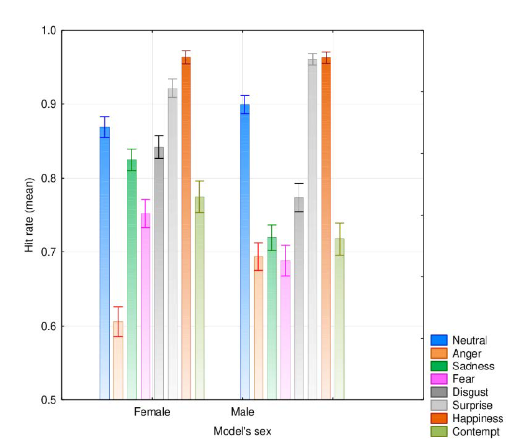
\includegraphics[width=1\linewidth]{facereqhuman.png}
                \caption{A különböző érzelmi kategóriák átlagos egyetértési aránya a modellek nemétől függően. Forrás: \cite{facerecresult}}
                \label{fig:humanfacerec}
        	\end{figure}
        
            Mint ahogy a(z) \ref{fig:humanfacerec}. ábra is szemlélteti, a tanulmány megállapította, hogy az érzelmek felismerése a női modelleken jobbnak bizonyult,
            a férfi modellekhez képest a szomorúság (82,5\%-os és 72,0\%-os átlagos egyetértési arány),
            félelem (átlagos egyetértési arányok 75,2\% és 68,8\%), undor (átlagos egyetértési arányok
            84,2\% és 77,4\%) és a megvetés (átlagos egyetértési arány 77,5\% és 71,8\%) esetében. Az egyetértési arányok azonban magasabbak voltak a férfi, mint a női modellekben az alábbi esetekben
            harag (69,4\% és 60,6\%), meglepettség (96,1\% és 92,2\%),
            és a semleges arc (89,9\% és 86,9\%). 
        
            Általánosságban elmondható, hogy a bemutatott és a felismert érzelmek közötti átlagos százalékos egyezés
            82\% volt.
    
            A(z) \ref{fig:fec-comparison}. táblázat tartalmazza az emberek által elért arckifejezés osztályozó feladat eredményeit összehasonlítva a saját mélytanuláson alapuló megvalósításunk eredményeivel.
    
            \begin{table}[htb]\centering
                        \begin{tabular}{lll}
                            Érzelmek    & \begin{tabular}[c]{@{}l@{}}Emberek találati aránya (\%) \end{tabular} & \begin{tabular}[c]{@{}l@{}} Hálózat találati aránya (\%)\end{tabular} \\
                            semleges & 88.4                                                          & 69                                                             \\
                            meglepődött & 94.2                                                          & 78                                                             \\
                            undor       & 80.9                                                           & 80                                                             \\
                            boldogság   & 96.8                                                          & 85                                                            \\
                            félelem     & 73.8                                                          & 59                                                            \\
                            szomorúság  & 76.2                                                          & 53                                                            \\
                            mérges      & 67.7                                                          & 51                                                            
                        \end{tabular}
                        \caption{Az emberek által elért arckifejezés osztályozó feladat eredményei összehasonlítva a saját mélytanuláson alapuló megvalósításunk eredményeivel.}
                        \label{fig:fec-comparison}
                    \end{table}
        

        \begin{figure}[h]	
    		\centering
    		\includegraphics[width=1\linewidth]{facerechuman-confmatrix.png}
            \caption{A "találati arányok" átlaga és szórása (SD) arckifejezésenként (\%). Forrás: \cite{facerecresult}}
            \label{fig:humanfacerecmatrix}
    	\end{figure} 

        \clearpage

        A(z) \ref{fig:humanfacerecmatrix}. (felmérés) és a \ref{fig:cfmatrix}. (saját megvalósítás) ábrákról az alábbi következtetések vonhatók le:

        \begin{itemize}
            \item A mérges arckifejezést az emberekhez hasonlóan a mélytanuláson alapuló megoldásunk is gyakran összetéveszti más érzelmi állapotokkal, mint például a félelemmel és a szomorúsággal.
            \item A meglepődöttséget a félelemmel téveszti össze a rendszerünk, csakúgy mint az emberekkel készített felmérésben.
            \item A saját megvalósításunk tanításához jóval több címkézett adatra lenne szükségünk, annak érdekében, hogy jobban hasonlítsanak a számszerűsített eredményeink a valósághoz.
        \end{itemize}

        \subsection{Arcrekonstrukció}
        \begin{figure}[htb]
                \centering
                 \begin{subfigure}[b]{1\textwidth}
                   \includegraphics[width=1\linewidth]{ruben_vis.jpg}
                \end{subfigure}

                \begin{subfigure}[b]{1\textwidth}
                   \includegraphics[width=1\linewidth]{hua_vis.jpg}
                \end{subfigure}
                
                \begin{subfigure}[b]{1\textwidth}
                   \includegraphics[width=1\linewidth]{pique_vis.jpg}
                \end{subfigure}

        
                \caption{Rekonstrukciós eredmények. Balról jobbra: bemeneti kép, detektált arcpontok, arcpontok, pirossal jelölve a nem látható pontokat, durva rekonstrukció, részletes rekonstrukció, alaptextúra a fényviszonyokkal, mélységi térkép}
                \label{fig:our-reconstruction-results}
            \end{figure}
            
            \begin{figure}[htb]
                \centering

                \begin{subfigure}[b]{1\textwidth}
                   \includegraphics[width=1\linewidth]{test0019_vis.jpg}
                \end{subfigure}

                \begin{subfigure}[b]{1\textwidth}
                   \includegraphics[width=1\linewidth]{test0021_vis.jpg}
                \end{subfigure}

                \begin{subfigure}[b]{1\textwidth}
                   \includegraphics[width=1\linewidth]{test0023_vis.jpg}
                \end{subfigure}

                \begin{subfigure}[b]{1\textwidth}
                   \includegraphics[width=1\linewidth]{test0027_vis.jpg}
                \end{subfigure}

                \begin{subfigure}[b]{1\textwidth}
                   \includegraphics[width=1\linewidth]{test0029_vis.jpg}
                \end{subfigure}

                \begin{subfigure}[b]{1\textwidth}
                   \includegraphics[width=1\linewidth]{test0030_vis.jpg}
                \end{subfigure}
                
                \caption{Rekonstrukciós eredmények. Balról jobbra: bemeneti kép, detektált arcpontok, arcpontok, pirossal jelölve a nem látható pontokat, durva rekonstrukció, részletes rekonstrukció, alaptextúra a fényviszonyokkal, mélységi térkép}
                \label{fig:our-reconstruction-results2}
            \end{figure}

            \begin{figure}[htb]
                \centering
                \includegraphics[width=.3\textwidth]{ruben_3d.jpg}\hfill
                \includegraphics[width=.3\textwidth]{hua_3d.jpg}\hfill
                \includegraphics[width=.3\textwidth]{pique_3d.jpg}
                
                \includegraphics[width=.3\textwidth]{19_3d.jpg}\hfill
                \includegraphics[width=.3\textwidth]{21_3d.jpg}\hfill
                \includegraphics[width=.3\textwidth]{23_3d.jpg}
                
                \includegraphics[width=.3\textwidth]{27_3d.jpg}\hfill
                \includegraphics[width=.3\textwidth]{29_3d.jpg}\hfill
                \includegraphics[width=.3\textwidth]{30_3d.jpg}
                
                \caption{Rekonstruált 3D modellek textúrával.}
                \label{fig:rekonstructed-faces}
            \end{figure}

            \begin{figure}[h]	
    		      \centering
    		      \includegraphics[width=1\linewidth]{focus_visual_results.jpg}
                \caption{A FOCUS modell eredményei. (Fentről lefelé: bemeneti
                képek, a rekonstrukciós képeink és a becsült maszkok.) Forrás: \cite{focus}}
                \label{fig:focusvisres}
    	       \end{figure} 

             \begin{figure}[h]	
    		      \centering
    		      \includegraphics[width=1\linewidth]{deca_results2.png}
                \caption{A DECA modell eredményei. (Fentről lefelé: bementi kép, durva rekonstrukció, részletes rekonstrukció.) Forrás: \cite{deca}}
                \label{fig:decavisres}
    	       \end{figure} 
            \clearpage

            A(z) \ref{fig:our-reconstruction-results}. és a(z) \ref{fig:our-reconstruction-results2}. ábrák a rekonstrukciós eredményeinket szemléltetik. Az egyes sorokban a képek balról jobbra haladva tartalmazzák a bemeneti képet, a detektált arcpontokat zöld színnel jelölve, pirossal jelölve a nem látható pontokat, a durva rekonstrukciót, a részletes rekonstrukciót, az
            alaptextúrát hozzáadott megvilágítással, valamint a mélységi térképet.
            A(z) \ref{fig:our-reconstruction-results}. ábra felső két sora a csapatunk tagjairól készült eredményeket tartalmazza, míg a többi kép a CelebA teszthalmazából származik.

            A(z) \ref{fig:rekonstructed-faces}. ábra tartalmazza az arcrekonstrukciós modellünk által generált 3D rekonstrukciókat a saját textúrájukkal.

            Mint láthatjuk a(z) \ref{fig:decavisres}. ábrán, a DECA által készített 3D-s modell sokkal részletesebben tudja rekonstruálni a személyspecifikus jellegzetes arcvonulatukat a mi (\ref{fig:our-reconstruction-results}. ábra) modellünkhöz képest, mivel Yao Feng és tsai. a modelljüket 3 lépésben tanították. Az első lépés az előtanítás, majd a durva alak kinyerése és a részletes adatok kinyerése következett a tanítás során. Míg a mi megoldásunkban csak az első két lépést végeztül el. Ennek oka az erőforrás és a tanító adatok hiánya.

            A saját eredményeinken (\ref{fig:rekonstructed-faces}. ábra) megfigyelhető, hogy néhány arcrekonstrukciónál minimálisan eltér az arcok textúrája. Úgy gondoljuk, hogy ennek oka a bemeneti képek nem teljes mértékben megfelelő előfeldolgozása lehet.

            A(z) \ref{fig:focusvisres}. ábra vizsgálata során megfigyelhetjük, hogy a FOCUS által produkált eredmények sikeresen kimaszkolták az eltakarásokat. Azonban a mi rekonstrukciónk során még mindig jelen vannak az arcot kitakaró tényezők, ahogy az a \ref{fig:rekonstructed-faces}. ábrán is látható. Miután körültekintően vizsgáltuk az okokat, arra a következtetésre jutottunk, hogy szükséges a hálózat további tanítása.
            
            \clearpage
            \subsubsection{NOW evaluáció}

            A NoW teljesítményértékelést az egyetlen monokuláris képből történő 3D arc rekonstrukciós módszerek kiértékelésére hozták létre Sanyal és tsai. \cite{now} A teljesítményértékelés célja egy szabványos értékelési metrika bevezetése a 3D arcrekonstrukciós módszerek pontosságának és robusztusságának mérésére a látószög, a megvilágítás és az általános eltakarások változásai mellett.

            A kihívás egyetlen monokuláris kép alapján egy 3D-s arc rekonstruálása. Mivel a megjósolt háló különböző helyi koordinátarendszerekben fordul elő, a rekonstruált 3D hálót mereven a szkenneléshez igazítják (azaz forgatják, eltolják és opcionálisan skálázzák), a rekonstruált kép és a szkennelés közötti megfelelő tájékozódási pontok segítségével. A merev igazítást a szkennelés-háló távolság (amely az egyes szkennelési csúcsok és a hálófelület legközelebbi pontja közötti abszolút távolság) alapján végzik el az alapigazság-szkennelés és a rekonstruált háló között, a tájékozódási pontok igazításával.

            Ahhoz, hogy tudjuk számszerűsíteni a módszerünk teljesítményét, a NoW Challenge GitHub oldalán ($https://github.com/soubhiksanyal/now_evaluation$) lévő utasításokat követve, le kellett futtatnunk különböző python szkripteket, amely során kiszámítják a hibamértékeket, és azokból összeállítanak egy halmozott hibadiagramot.
            
            A módszerek teljesítményét a megjósolt 3D arcmodell és az alapigazság 3D arcmodell közötti hiba mediánja, átlaga és szórása(std) alapján mérjük milliméterben. 
            
            \begin{table}[htb]\centering
            \begin{tabular}{llll}
            \multicolumn{4}{c}{Now eredmények}                 \\
                             & medián(mm) & átlag(mm) & szórás(mm) \\
            DECA             & 1.04       & 1.30     & 1.10    \\
            FOCUS            & 1.09       & 1.38     & 1.18    \\
            A mi eredményünk & 1.27       & 1.62     & 1.38   
            \end{tabular}
            \caption{A DECA és a FOCUS eredményei összehasonlítva a saját megvalósításunkkal.}
            \end{table}

            \begin{figure}[h]	
    		      \centering
    		      \includegraphics[width=1\linewidth]{cummulative-error.png}
                \caption{Halmozott hibadiagram. Az X tengely az alapigazság 3D modelltől való eltérést jelöli milliméterben, míg az Y tengely a hibák halmozott eloszlását a tesztadatokon, százalékban kifejezve. A kék szinű görbe a mi megoldásunkat jelképezi, a narancssárga a FOCUS \cite{focus}, és a zöld a DECA \cite{deca}.}
                 \label{fig:cummulative-error}
    	    \end{figure} 

            A(z) \ref{fig:cummulative-error}. ábrán látható diagram azt mutatja meg, hogy összes vizsgálati minta hány százaléka milyen hiba tartományba esik. Ebből következtetve, minél meredekebb a görbe, annál jobban teljesít a módszer.
    
    \section{A megvalósítás elemzése}

        Az általunk megvalósított arcrekonstrukciós modell eredményeit vizsgálva azt láthatjuk, hogy a modellünk kevés adattal is sikeresen rekonstruál 3D-s arcképeket. Azonban a rekonstruált arcképek minősége elmarad a már publikált kutatások eredményeitől. Ez részben annak tudható be, hogy alacsony erőforrásokhoz kellett igazítanunk a modellünket. Ugyanakkor úgy gondoljuk, hogy további kutatói munkával, több adattal és jobb optimalizációval a modellünk teljesítménye jelentősen javulhat. Az eredményeink azt sugallják, hogy a modellünk továbbfejlesztése nagyobb adatmennyiség és finomhangolás által nagyobb teljesítményt érhet el a jövőben. 

        Az arcanalízis modellünk teljesítményének értékelésekor arra jutottunk, hogy nem éri el az emberi szintet. Ugyanakkor megfigyeltük, hogy bizonyos érzelmeket mégis nagy pontossággal képes felismerni. Az eredményeink alapján azt gondoljuk, hogy a modellünk hiányos tanító adatokkal rendelkezik, amely korlátozza a teljesítményét. Ennek fényében javasoljuk, hogy a tanító adatbázisunk bővítése segíthetne a modellünk pontosságának javításában.
    
        \subsection{Alkalmazások}

        A 3D arcrekonstrukciós és az érzelem felismerő hálózatok együttes alkalmazása számos területen alkalmazható, beleértve az virtuális valóság (VR), bűnüldözés, marketing és szórakoztató ipar területeit. 
        
        Az egyik felhasználási lehetőség egy olyan alkalmazás, amely lehetővé teszi, hogy az emberek virtuálisan próbálhassanak fel ruhákat, kiegészítőket vagy ékszereket. A 3D arcrekonstrukciós hálózat felhasználható lenne az arcok pontosságával és élethűségével, míg az érzelem felismerő hálózat meghatározná az éppen vásárló kedvenc termékét vagy annak ellenkezőjét, és ennek megfelelően javaslatokat adna a további vásárlásra.

        Alkalmazásuk hasznos lehet klinikai vizsgálatokban is.
        Például az érzelmek felismerése és az arcok élethű rekonstrukciója segíthet az orvosoknak azonosítani azokat a tüneteket, amelyeket a betegek arckifejezései mutatnak, például az arcfájdalmat vagy a depressziót. Az arcrekonstrukciós hálózat segítségével az orvosok pontosabb diagnózist adhatnak, az érzelem felismerő hálózat pedig segíthet az orvosoknak megérteni a beteg állapotát és javaslatokat adni az esetleges kezelésre.

        Bár a 3D arcrekonstrukció és az érzelem- és nemfelismerés rendszerekben óriási potenciált láthatunk, fontos figyelembe venni a velük járó hátrányokat is. Az ilyen alkalmazásoknak társadalmi kockázata lehet a magánélet és az adatvédelem sérülése, hiszen az ilyen technológiák lehetővé teszik az egyének könnyű és pontos azonosítását, amely miatt felmerülhet a személyes adatok jogosulatlan felhasználása. Az ilyen technológiák használata további etikai és jogi kihívásokat is felvet, amelyeket meg kell oldani a biztonságos és felelős használat érdekében.
            
        \subsection{Továbbfejlesztési lehetőségek}

        A továbbfejlesztési lehetőségeink közé tartozik a Kubernetes klaszter konfigurálása és a mikroszerviz komponensek kitelepítése. Ez javítani fogja a rendszerünk skálázhatóságát és megbízhatóságát. Az új rendszerünk monitorozó és logoló rendszereket is tartalmaz majd, amelyek segítségével a rendszer működése könnyen követhető és hibakeresési lehetőségeink is bővülnek.

        Az arcanalízis hálózatunk továbbfejlesztése szintén fontos szerepet játszik a jövőbeli terveinkben. A tanító adathalmazunk bővítésével és a hiperparaméterek optimalizálásával további javulást várunk a hálózat teljesítményében. Ezenkívül az API megtervezése is tervben van.

        Az arcrekonstrukciós hálózatunk fejlesztése is folytatódni fog. Az első lépés a tanító adathalmazunk kibővítése lesz, majd a hiperparaméterek további finomhangolása. Az erőforrások függőleges skálázása is fontos, hogy a rendszer hatékonyan tudjon dolgozni a nagyobb adathalmazokkal. A tanítás során felhasznált veszteségfüggvények halmazának kibővítése és optimalizálása szükséges lesz a részletesebb 3D arcrekonstrukció eléréséhez.

        Végül az új mikroszerviz architektúránk end-to-end tesztelése is szerepel a terveink között. Ez segít majd azonosítani az esetleges hibákat, és biztosítani fogja a rendszerünk teljes funkcionalitását. Összességében ezek a továbbfejlesztési lehetőségek javítani fogják a rendszerünk hatékonyságát, teljesítményét és megbízhatóságát.

    \section{Tartalmi összefoglaló és következtetések}

        A munkánk célja egy realisztikus 3D arcrekonstrukciós hálózat, egy hét különböző érzelem felismerésére alkalmas hálózat, valamint egy nemek felismerésére szolgáló hálózat létrehozása volt. Ezekhez a hálózatokhoz egy mikroszerviz architektúrára épülő felhasználóbarát webes alkalmazást is megterveztünk.
        
        A kutatás során többek között megvizsgáltuk a neurális hálózatok egyes típusainak felépítését, tanítási lehetőségeit, valamint az arcrekonstrukciós lehetőségeket. A kapcsolódó kutatásokat is alaposan elemeztük, beleértve a DECA és FOCUS modelleket, valamint az ezekben alkalmazott renderelési módszereket és arcpont felismerő hálózatokat.
        
        Az alkalmazás tervezése során az első lépés a rendszerterv megalkotása volt. 
        A rendszer két fő része az arcrekonstrukciós és arcanalizáló modul. Ezeken kívül
        egy React.js frontendből, egy Java backendből és egy MongoDB adatbázisból áll.
        
        Részletesen bemutattuk az arcrekonstrukciós és az arcanalizáló hálózatok megvalósítását, 
        beleértve az egyes rétegek felépítését és a tanítási folyamatokat. Az alkalmazás tesztelése során az eredményeket összehasonlítottuk a meglévő megvalósításokkal.

        Természetesen a személyes cél is nagy szerepet játszott a kutatás során, hiszen a csapat tagjainak fő motivációja az volt, hogy megismerjék és kipróbálják a különböző technológiákat, különös tekintettel a mesterséges intelligencia által nyújtott lehetőségeket.

        Az elért eredmények bemutatása és azok összehasonlítása meglévő megvalósításokkal kiemelkedő fontosságú volt ahhoz, hogy lássuk, milyen előnyöket biztosít az általunk kifejlesztett rendszer. Az eredmények alapján megállapítható, hogy kutatásunk céljait nagyrészt elérte, és a létrehozott rendszerünk pontos és hatékony arcrekonstrukciót és arcanalízist biztosít a felhasználók számára. A fejlesztés során megismertük a különböző keretrendszereket és azok használatát, ezáltal személyes céljainkat is elértük.

    \section{Summary of contents and conclusions}

        The aim of our work was to create a realistic 3D face reconstruction network, a network for the recognition of seven different emotions and a network for sex recognition. For these networks, we also designed a user-friendly web application based on a microservice architecture.
    
        Among other things, the research investigated the structure of different types of neural networks, their learning approaches, and face reconstruction possibilities. Related research has also been thoroughly analysed, including DECA and FOCUS models and the rendering methods and face recognition networks used in them.

        The first step was to create a system design. 
        The two main parts of the system are the face reconstruction and face analysis modules. In addition to these, the system contains a React.js frontend, a Java backend and a MongoDB database.

        We have discussed the implementation of face reconstruction and face analysis networks in detail, 
        including the structure of each layer and the learning process. The results of the evaluation of the application were compared with existing implementations.

        As a matter of fact, a personal goal also played a big part in the research, as the main motivation for the team members was to learn about and try out different technologies, especially the possibilities offered by artificial intelligence.

        Demonstrating the results achieved and comparing them with existing implementations was of paramount importance to see the benefits of the system we developed. Based on the results, it can be concluded that the objectives of our research have been largely achieved and that the system we have created provides users with accurate and efficient facial reconstruction and facial analysis. During the development, we have learned about the different frameworks and their usage, thus achieving our personal goals.
        
    \newpage
    \section{Irodalomjegyzék}
	\renewcommand{\refname}{Hivatkozások}
	\begin{thebibliography}{9}
		
		\bibitem{tewari}
		Tewari, A., Zollhofer, M., Kim, H., Garrido, P., Bernard, F., Perez,
		P., Theobalt, C. (2017).
		\textit{Mofa: Model-based deep convolutional face au-
		toencoder for unsupervised monocular reconstruction. In Proceedings of
		the IEEE International Conference on Computer Vision Workshops (pp.
		1274-1283)}
		
		\bibitem{tran}
		Tuan Tran, A., Hassner, T., Masi, I., Medioni, G. (2017). 
		\textit{Regressing
		robust and discriminative 3D morphable models with a very deep neural
		network. In Proceedings of the IEEE conference on computer vision and
		pattern recognition (pp. 5163-5172)}
		
		\bibitem{olszewski}
		Olszewski, K., Lim, J. J., Saito, S., Li, H. (2016).
		\textit{High-fidelity facial and
		speech animation for VR HMDs. ACM Transactions on Graphics (TOG),
		35(6), 1-14}
		
		\bibitem{styner}
		Styner, M. A., Rajamani, K. T., Nolte, L. P., Zsemlye, G., Székely, G.,
		Taylor, C. J., Davies, R. H. (2003, July).
		\textit{ Evaluation of 3D correspondence
		methods for model building. In Biennial International Conference on In-
		formation Processing in Medical Imaging (pp. 63-75). Springer, Berlin,
		Heidelberg}
		
		\bibitem{survey} 
		Morales, A., Piella, G., Sukno, F. M. (2021). 
		\textit{Survey on 3D face re-
		construction from uncalibrated images. Computer Science Review, 40,
		100400.}
		
		\bibitem{auto}
		Kala, R. (2016).
		\textit{On-road intelligent vehicles: Motion planning for intel-
		ligent transportation systems. Butterworth-Heinemann.}	
		
		\bibitem{scanner}
		Kovacs, L., Zimmermann, A., Brockmann, G., Gühring, M., Baurecht,H., Papadopulos, N. A., ... Zeilhofer, H. F. (2006).
		\textit{Three-dimensional
		recording of the human face with a 3D laser scanner. Journal of plastic,
		reconstructive and aesthetic surgery, 59(11), 1193-1202}
		
		\bibitem{blanzvetter}
		Blanz, V., Vetter, T. (1999, July).
		\textit{A morphable model for the synthesis
		of 3D faces. In Proceedings of the 26th annual conference on Computer
		graphics and interactive techniques (pp. 187-194)}
		
		\bibitem{3dmm}
		Egger, B., Smith, W. A., Tewari, A., Wuhrer, S., Zollhoefer, M., Beeler,
		T.,... Vetter, T. (2020).
		\textit{3d morphable face models—past, present, and
		future. ACM Transactions on Graphics (TOG), 39(5), 1-38}
		
		\bibitem{dolphins}
		Cashman, T. J., Fitzgibbon, A. W. (2012).
		\textit{What shape are dolphins?
		building 3d morphable models from 2d images. IEEE transactions on pat-
		tern analysis and machine intelligence, 35(1), 232-244}
		
		\bibitem{photometric}
		Ackermann, J., Goesele, M. (2015).
		\textit{A survey of photometric stereo
			techniques. Foundations and Trends® in Computer Graphics and Vision,
			9(3-4), 149-254, 149–254.}
		
		\bibitem{multiplex}
		Hernández, C., Vogiatzis, G., Brostow, G. J., Stenger, B., Cipolla,
		R. (2007, October).
		\textit{Non-rigid photometric stereo with colored lights. In
			2007 IEEE 11th International Conference on Computer Vision (pp. 1-8).
			IEEE}
		
		\bibitem{hibrid}
		Nehab, D., Rusinkiewicz, S., Davis, J., Ramamoorthi, R. (2005).
		\textit{Efficiently combining positions and normals for precise 3D geometry. ACM transactions on graphics (TOG), 24(3), 536-543.}
			
		\bibitem{patelsmith}
		Patel, A., Smith, W. A. (2012).
		\textit{Driving 3D morphable models using shading cues. Pattern Recognition, 45(5), 1993-2004}
		
		\bibitem{ann}
		Abraham, A. (2005).
		\textit{Artificial neural networks. Handbook of measuring system design}
		
		\bibitem{ann2}
		Jain, A. K., Mao, J., Mohiuddin, K. M. (1996).
		\textit{Artificial neural networks: A tutorial. Computer, 29(3), 31-44}
		
		\bibitem{ann3}
		\textit{MARCELL, Borza. Mesterséges neurális hálózatok matematikai alapjai.}
		
		\bibitem{ann4}
		Tamás, K. (2002).
		\textit{A mesterséges neurális hálók a jövőkutatás
			szolgálatában.}
		
		\bibitem{krenker}
		Krenker, A., Bester, J., Kos, A. (2011).
		\textit{Introduction to the artificial neural networks. Artificial Neural Networks: Methodological Advances and
			Biomedical Applications. InTech, 1-18.}
		
		\bibitem{saragih}
		Saragih, J. M., Lucey, S., Cohn, J. F. (2011, March). 
		\textit{Real-time avatar
			animation from a single image. In 2011 IEEE International Conference
			on Automatic Face and Gesture Recognition (FG) (pp. 117-124). IEEE}
		
		\bibitem{CNN}
		Indolia, S., Goswami, A. K., Mishra, S. P., Asopa, P. (2018).
		\textit{ Conceptual
			understanding of convolutional neural network-a deep learning approach.
			Procedia computer science, 132, 679-688.}
	
	
	\bibitem{synthetic}
	Richardson, E., Sela, M., Kimmel, R. (2016, October). 
	\textit{3D face reconstruction by learning from synthetic data. In 2016 fourth international conference on 3D vision (3DV) (pp. 460-469). IEEE.}
	
	\bibitem{keras}
	Manaswi, N. K. (2018).
	\textit{Understanding and working with Keras. In Deep
		Learning with Applications Using Python (pp. 31-43). Apress, Berkeley,
		CA.}
	
	\bibitem{yudong}
	Guo, Y., Cai, J., Jiang, B., Zheng, J. (2018).
	\textit{Cnn-based real-time
		dense face reconstruction with inverse-rendered photo-realistic face images. IEEE transactions on pattern analysis and machine intelligence,
		41(6), 1294-1307.}
	
	\bibitem{elad}
	 Richardson, E., Sela, M., Kimmel, R. (2016, October).
	\textit{3D face reconstruction by learning from synthetic data. In 2016 fourth international conference on 3D vision (3DV) (pp. 460-469). IEEE.}
	
	\bibitem{yudeng}
	Deng, Y., Yang, J., Xu, S., Chen, D., Jia, Y., Tong, X. (2019).
	\textit{Accurate
		3d face reconstruction with weakly-supervised learning: From single image
		to image set. In Proceedings of the IEEE/CVF Conference on Computer
		Vision and Pattern Recognition Workshops (pp. 0-0)}
	
	\bibitem{chen}
	Chen, D., Hua, G., Wen, F., Sun, J. (2016, October). 
	\textit{Supervised transformer network for efficient face detection. In European Conference on
		Computer Vision (pp. 122-138). Springer, Cham.}
	
	\bibitem{kingma}
	Kingma, D. P., Ba, J. (2014).
	\textit{Adam: A method for stochastic optimization. arXiv preprint arXiv:1412.6980.}
	
	\bibitem{deca}
	Feng, Y., Feng, H., Black, M. J., Bolkart, T. (2021).
	\textit{Learning an animatable detailed 3D face model from in-the-wild images. ACM Transactions
		on Graphics (TOG), 40(4), 1-13.}
	
	\bibitem{focus}
	Li, C., Morel-Forster, A., Vetter, T., Egger, B., Kortylewski, A. (2021).
	\textit{To fit or not to fit: Model-based Face Reconstruction and Occlusion Segmentation from Weak Supervision. arXiv preprint arXiv:2106.09614.}
	
	\bibitem{flame}
	Tianye Li, Timo Bolkart, Michael. J. Black, Hao Li, and Javier Romero
	(2017).
	\textit{Learning a model of facial shape and expression from 4D scans.
		ACM Transactions on Graphics, (Proc. SIGGRAPH Asia) 36, 6 (2017),
		194:1–194:17.}
	
	\bibitem{liwen}
	Liwen Hu, Shunsuke Saito, Lingyu Wei, Koki Nagano, Jaewoo Seo, Jens
	Fursund, Iman Sadeghi, Carrie Sun, Yen-Chun Chen, and Hao Li. (2017).
	(2017).
	\textit{Avatar Digitization from a Single Image for Real-time Rendering. ACM
		Transactions on Graphics (TOG) 36, 6 (2017), 195:1–195:14.}
	
	\bibitem{bulat}
	Adrian Bulat and Georgios Tzimiropoulos (2017).
	\textit{How far are we from solving the 2D and 3D Face Alignment problem? (and a dataset of 230,000 3D facial landmarks). In International Conference on Computer Vision.}
	
	\bibitem{mohammed}
	Mohammed, S. B., Abdulazeez, A. M. (2021).
	\textit{Deep Convolution Neural
		Network for Facial Expression Recognition. PalArch’s Journal of Archaeology of Egypt/Egyptology, 18(4), 3578-3586.}
	
	\bibitem{arcface}
	Deng, J., Guo, J., Xue, N., and Zafeiriou, S. (2019).
	\textit{Arcface: Additive angular margin loss for deep face recognition. In Proceedings of the
		IEEE/CVF conference on computer vision and pattern recognition (pp.
		4690-4699).}
	
	\bibitem{feafa}
	Yan, Y., Lu, K., Xue, J., Gao, P., and Lyu, J. (2019, July).
	\textit{Feafa: A
		well-annotated dataset for facial expression analysis and 3d facial animation. In 2019 IEEE International Conference on Multimedia and Expo
		Workshops (ICMEW) (pp. 96-101). IEEE.}
	
	\bibitem{paysan}
	Paysan, P., Knothe, R., Amberg, B., Romdhani, S., and Vetter, T. (2009, September).
	\textit{A 3D face model for pose and illumination invariant
		face recognition. In 2009 sixth IEEE international conference on advanced
		video and signal based surveillance (pp. 296-301). Ieee.}

    \bibitem{PCA}
	Castelán, Mario, and Edwin R. Hancock.
	\textit{A simple coupled statistical model for 3d face shape recovery. 18th International Conference on Pattern Recognition (ICPR'06). Vol. 1. IEEE, 2006.}


    \bibitem{resnet}
	Kaiming He, Xiangyu Zhang, Shaoqing Ren, and Jian Sun.
	\textit{Deep Residual Learning for Image Recognition. In IEEE Conference on Computer Vision and Pattern Recognition  2016. (CVPR). 770–778.}

    \bibitem{tl}
    Weiss, Karl, Taghi M. Khoshgoftaar, and DingDing Wang.
    \textit{A survey of transfer learning." Journal of Big data 3.1 (2016): 1-40.}

    \bibitem{unet}
    Olaf Ronneberger, Philipp Fischer, and Thomas Brox.
    \textit{U-net: Convolutional networks for biomedical image segmentation. In International Conference on Medical image computing and computer-assisted intervention. Springer, 234–241 (2015.)}

    \bibitem{celeba}
    Liu, Z., Luo, P., Wang, X., Tang, X.
    \textit{Deep learning face attributes in the wild. In: Proceedings of the IEEE international conference on computer vision. 2015. p. 3730-3738.}

    \bibitem{ciresan}
    Ciresan, D.C., Gambardella, L.M., Giusti, A., Schmidhuber, J.
    \textit{Deep neural networks segment neuronal membranes in electron microscopy images. In: NIPS, pp. 2852–2860 (2012)}

    \bibitem{diffrenderer}
    Kato, Hiroharu, et al.
    \textit{Differentiable rendering: A survey. arXiv preprint arXiv:2006.12057 (2020).}

    \bibitem{facerecresult}
    Dores, Artemisa R., et al.
    \textit{Recognizing emotions through facial expressions: A largescale experimental study. International journal of environmental research and public health 17.20 (2020): 7420.}

    \bibitem{pretrained-resnet}
    Xuan Cao, Zhang Chen, Anpei Chen, Xin Chen, Shiying Li, and Jingyi Yu. 2018a.
    \textit{Sparse Photometric 3D Face Reconstruction Guided by Morphable Models. In    IEEE Conference on Computer Vision and Pattern Recognition (CVPR). 4635–4644.}

    \bibitem{regularization-survey}
    Tian, Yingjie, and Yuqi Zhang.
    \textit{A comprehensive survey on regularization strategies in machine learning. Information Fusion 80 (2022): 146-166.}

    \bibitem{now}
    Sanyal, Soubhik, et al.
    \textit{Learning to regress 3D face shape and expression from an image without 3D supervision. In: Proceedings of the IEEE/CVF Conference on Computer Vision and Pattern Recognition. 2019. p. 7763-7772.}
    

    \bibitem{ruder}
    Ruder, Sebastian
    \textit{An overview of gradient descent optimization algorithms. arXiv preprint arXiv:1609.04747, 2016.}

    \bibitem{standard-rasterizer}
    Scratchapixel.
    \textit{"Overview of the Rasterization Algorithm." Scratchapixel, n.d., \url{https://www.scratchapixel.com/lessons/3d-basic-rendering/rasterization-practical-implementation/overview-rasterization-algorithm.html}. Accessed 8 May 2023.}

    \bibitem{lbs}
    Jeruzalski, Timothy, et al.
    \textit{"Nilbs: Neural inverse linear blend skinning." arXiv preprint arXiv:2004.05980 (2020).}


	\end{thebibliography}
 \end{document}